\begin{savequote}[75mm]
Calculus required continuity, and continuity was supposed to require the infinitely little; but nobody could discover what the infinitely little might be.      
\qauthor{--- Bertrand Russell ---}
\end{savequote}

\chapter{Vector calculus}
\graphicspath{{figures/Vector_Calc/}}

\section{Line integrals over a scalar field}\label{sec:line_int_intro}
This section explores completely different relationships between vectors and integration. These relationships will enable us to compute the work done by a magnetic field in moving an object along a path and find how much air moves through an oddly--shaped screen in space, among other things. 

\subsection{Definition}
Consider the surface and curve shown in Figure \ref{fig_Vector_Calc_1a}. The surface is given by $$f(x,y)=1-\cos(x)\sin(y).$$
The dashed curve lies in the $xy$-plane and is the familiar $y=x^2$ parabola from $-1\leq x\leq1$; we will call this curve $C$. The curve drawn with a solid line in the graph is the curve in space that lies on our surface with $x$- and $y$- values that lie on $C$. 

The question we want to answer is this: what is the area that lies below the curve drawn with the solid line? In other words, what is the area of the region above $C$ and under the surface $f$? This region is shown in Figure \ref{fig_Vector_Calc_1b}. We suspect the answer can be found using an integral, but before trying to figure out what that integral is, let us first try to approximate its value. 


\begin{figure}[t]
\centering
%\raisebox{0.5cm}{
\subfigure[\label{fig_Vector_Calc_1a}]{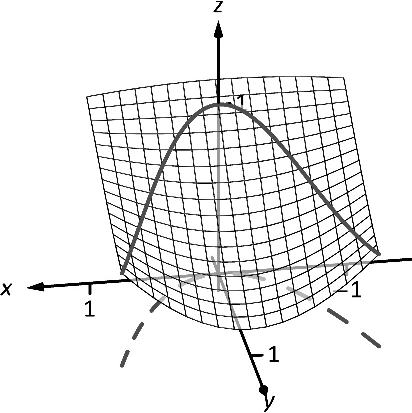
\includegraphics[width=0.33\textwidth]{fig_Vector_Calc_1a}}
\qquad
\subfigure[\label{fig_Vector_Calc_1b}]{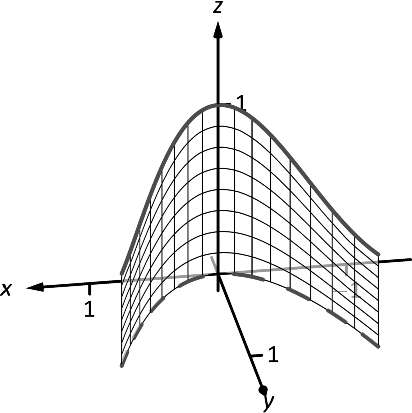
\includegraphics[width=0.33\textwidth]{fig_Vector_Calc_1b} }
\qquad
\subfigure[\label{fig_Vector_Calc_1c}]{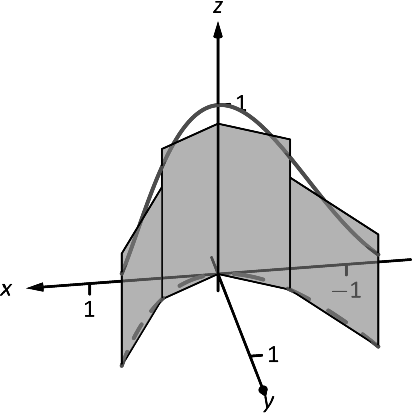
\includegraphics[width=0.33\textwidth]{fig_Vector_Calc_1c} }
\caption{Finding area under a curve in space.}
\end{figure}


In Figure \ref{fig_Vector_Calc_1c}, four rectangles have been drawn over the curve $C$. The bottom corners of each rectangle lie on $C$, and each rectangle has a height given by the function $f(x,y)$ for some $(x,y)$ pair along $C$ between the rectangle's bottom corners. 
As we know how to find the area of each rectangle, we are able to approximate the area above $C$ and under $f$. Clearly, our approximation will be an approximation. The heights of the rectangles do not match exactly with the surface $f$, nor does the base of each rectangle follow perfectly the path of $C$.

In typical calculus fashion, our approximation can be improved by using more rectangles. The sum of the areas of these rectangles gives an approximate value of the true area above $C$ and under $f$. As the area of each rectangle is height $\times$ width, we assert that the
$$\text{area above $C$}\approx \sum (\text{heights}\times\text{widths}).$$

When first learning of the integral, and approximating areas with (heights $\times$ widths), the width was a small change in $x$: $dx$. That will not suffice in this context. Rather, each width of a rectangle is actually approximating the arc length of a small portion of $C$. In Section \ref{sec:curvature}, we used $s$ to represent the arc length parameter of a curve. Hence, a small amount of arc length will thus be represented by $ds$. 

The height of each rectangle will be determined in some way by the surface $f$. If we parametrize $C$ by $s$, an $s$-value corresponds to an $(x,y)$ pair that lies on the parabola $C$. Since $f$ is a function of $x$ and $y$, and $x$ and $y$ are functions of $s$, we can say that $f$ is a function of $s$. Given a value $s$, we can compute $f(s)$ and find a height. Thus
\begin{align}
\text{area under $f$ and above $C$}&\approx \sum (\text{heights}\times\text{widths});\notag\\
		\text{area under $f$ and above $C$}							&=\lim_{\mathcal{L}\to0}\sum f(c_i)\Delta s_i\notag\\
									&=\int_Cf(s)\ ds.\label{eq:line0}
\end{align}

Here we have introduce a new notation, the integral symbol with a subscript of $C$. It is reminiscent of our usage of $\iint_R$. Using the train of thought found in the Integration Review preceding this section, we interpret $\int_C f(s)\ ds$ as meaning sum up, along a curve $C$, function values $f(s)$ $\times$ small arc lengths. It is understood here that $s$ represents the arc length parameter.

All this leads us to a definition. The integral found in Equation \ref{eq:line0} is called a \textbf{line integral}. We formally define it below.

\begin{definition}[Line integral over a scalar field]\label{def:line_integral1}
Let $C$ be a smooth curve parametrized by $s$, the arc length parameter, and let $f$ be a continuous function of $s$. A \textbf{line integral} (\textit{lijnintegraal}) is an integral of the form
$$\int_C f(s)\ ds = \lim_{\mathcal{L}\to 0}\sum_{i=1}^n f(c_i)\Delta s_i,$$
where $s_1<s_2<\cdots<s_n$ is any partition of the $s$-interval over which $C$ is defined, $c_i$ is any value in the $i\,^\text{th}$ subinterval,  $\Delta s_i$ is the width of the $i\,^\text{th}$ subinterval, and $\mathcal{L}$ is the length of the longest subinterval in the partition.\index{line integral}\index[aut]{lijnintegraal}%
\end{definition}

Note that Definition \ref{def:line_integral1} uses the term scalar field which has not yet been defined. Its meaning is discussed in  when it is compared to a vector field. Besides, when $C$ is a closed curve, i.e., a curve that ends at the same point at which it starts,  we use 
$$
\oint_C f(s)\ ds$$
instead of
$$
\quad \int_C f(s)\ ds.$$

The definition of the line integral does not specify whether $C$ is a curve in the plane or space (or hyperspace), as the definition holds regardless. For now, however, we will assume $C$ lies in the $xy$-plane.

Actually, this definition of the line integral  does not really say anything new. If $C$ is a curve and $s$ is the arc length parameter of $C$ on $a\leq s\leq b$, then 
$$\int_Cf(s)\ ds = \int\limits_a^bf(s)\ ds.$$
The real difference with this integral from the standard $\int\limits_a^bf(x)\ dx$ we used in the past is that of context. Our previous integrals naturally summed up values over an interval on the $x$-axis, whereas now we are summing up values over a curve. If we can parametrize the curve with the arc length parameter, we can evaluate the line integral just as before. Unfortunately, parametrizing a curve in terms of the arc length parameter is usually very difficult, so we must develop a method of evaluating line integrals using a different parametrization.

Given a curve $C$, find any parametrization of $C$: $x = g(t)$ and $y=h(t)$, for continuous functions $g$ and $h$, where $a\leq t\leq b$. We can represent this parametrization with a vector--valued function, \linebreak $\vrt = \left( g(t),h(t)\right)$.

In Section \ref{sec:curvature}, we defined the arc length parameter as 
$$
s(t) = \int\limits_0^t \norm{\vec r\,'(u)}\ du. 
$$
By the fundamental theorem of calculus, $ds = \norm{\vec r\,'(t)}\ dt$. We can substitute the right hand side of this equation for $ds$ in the line integral definition. Moreover, we can view $f$ as being a function of $x$ and $y$ since it is a function of $s$. Thus $f(s) =f(x,y) =f\big(g(t),h(t)\big)$. This gives us a concrete way to evaluate a line integral:
$$\int_C f(s)\ ds = \int\limits_a^bf\big(g(t),h(t)\big)\ \norm{\vec r\,'(t)}\ dt.$$

We restate this as a theorem for its $n$--dimensional analogue.

\begin{theorem}[Evaluating a line integral over a scalar field]\label{thm:line1}
Let $C$ be a curve parametrized by $\vrt =\left( g_1(t), g_2(t),\ldots,g_n(t)\right)$, $a\leq t\leq b$, where $g_i$ is continuously differentiable, and let $z=f(\mathbf{x})$, where $f$ is continuous over $C$. Then\index{line integral!over scalar field}%
	$$\int_Cf(s)\ ds = \int\limits_a^bf\big(g_1(t),g_2(t),\ldots,g_n(t)\big)\ \norm{\vec r\,'(t)}\ dt.$$
\end{theorem}


To be clear, the first point of Theorem \ref{thm:line1} can be used to find the area under a surface $z=f(x,y)$ and above a curve $C$. We will later give an understanding of the line integral when $C$ is a curve in space.

Let us do an example where we actually compute an area.

\begin{example}\label{ex_linescalarfield2}
Find the area under the surface $f(x,y) =\cos(x)+\sin(y)+2$ over the curve $C$, which is the segment of the line $y=2x+1$ on $-1\leq x\leq 1$, as shown in Figure \ref{fig_Vector_Calc_2}.

\begin{figure}[H]
\centering
%\raisebox{0.5cm}{
\subfigure[\label{fig_Vector_Calc_2a}]{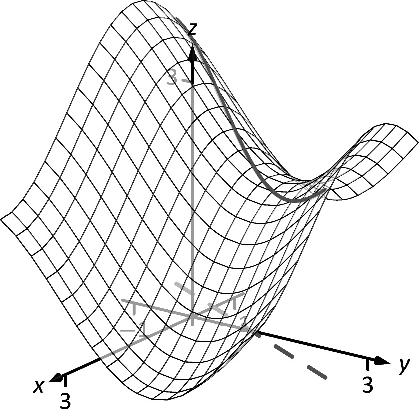
\includegraphics[width=0.43\textwidth]{fig_Vector_Calc_2a}}
\qquad
\subfigure[\label{fig_Vector_Calc_2b}]{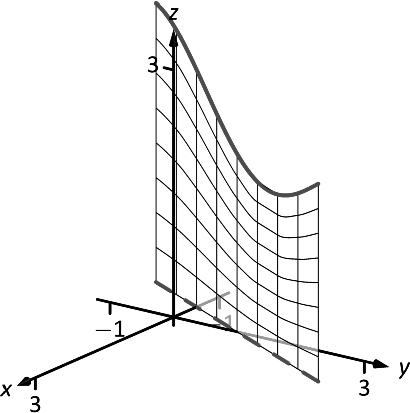
\includegraphics[width=0.43\textwidth]{fig_Vector_Calc_2b} }
\caption{Finding area under a curve in Example \ref{ex_linescalarfield2}.}
\label{fig_Vector_Calc_2}
\end{figure}

\pagebreak
\xhrulefill{gray}{2.5pt}Solution \xhrulefill{gray}{2.5pt}

Our first step is to represent $C$ with a vector--valued function. Since $C$ is a simple line, and we have a explicit relationship between $y$ and $x$ (namely, that $y=2x+1$), we can let $x = t$, $y = 2t+1$, and write $\vrt = \left( t, 2t+1\right)$ for $-1\leq t\leq 1$. 

We find the values of $f$ over $C$ as $$f(x,y) = f(t,2t+1) = \cos(t)+\sin(2t+1) + 2.$$ We also need \ $\norm{\vec r\,'(t)}$; with $\vrp(t) = \left(1,2\right)$, we have \ $\norm{\vrp(t)} = \sqrt{5}$. Thus $ds = \sqrt{5}\ dt$. 



The area we seek is 
\begin{align*}
\int_Cf(s)\ ds &= \int\limits_{-1}^1 \big(\cos(t)+\sin(2t+1) + 2\big)\sqrt{5}\ dt \\
					&= \left.\sqrt{5}\left(\sin(t) - \frac12\cos(2t+1)+2t\right)\right|_{-1}^1\\
					&\approx 14.418\ \text{units}^2.
\end{align*}



\end{example}

We now consider the example that introduced this section.\\

\begin{example}\label{ex_linescalarfield5}
Find the area under $f(x,y) = 1-\cos(x)\sin(y)$ and over the parabola $y = x^2$, from $-1\leq x\leq 1$. 

\xhrulefill{gray}{2.5pt}Solution \xhrulefill{gray}{2.5pt}

We parametrize our curve $C$ as $\vrt = \left( t,t^2\right)$ for $-1\leq t\leq 1$; we find $\norm{\vrp(t)} = \sqrt{1+4t^2}$, so $ds = \sqrt{1+4t^2}\ dt$. 

Replacing $x$ and $y$ with their respective functions of $t$, we have $$f(x,y) = f(t,t^2) = 1-\cos(t)\sin\left(t^2\right).$$ Thus the area under $f$ and over $C$ is found to be
$$
\int_C f(s)\ ds = \int\limits_{-1}^1 \Big(1-\cos(t)\sin\left(t^2\right)\Big)\sqrt{1+4t^2}\ dt.$$
This integral is impossible to evaluate using the techniques developed in this text. We resort to a numerical approximation; accurate to two places after the decimal, we find the area is 2.17.

\end{example}

Note how in each of the previous examples we are effectively finding area under a curve, just as we did when first learning of integration. We have used the phrase area over a curve $C$ and under a surface, but that is because of the important role $C$ plays in the integral. The figures show how the curve $C$ defines another curve on the surface $z=f(x,y)$, and we are finding the area under that curve.

\subsection{Properties}
Many properties of line integrals can be inferred from general integration properties. For instance, if $k$ is a scalar, then 
$$\int_C k\,f(s)ds = k\int_Cf(s)ds,$$
and similarly
$$\ds \int_C\big(f(s)+g(s)\big)\ ds = \int_Cf(s)\ ds +\int_Cg(s)\ ds,$$
where $f$ and $g$ are continuous functions of $s$.

One property in particular of line integrals is worth noting. If $C$ is a curve composed of subcurves $C_1$ and $C_2$, where they share only one point in common (see Figure \ref{fig_Vector_Calc_3a}), then the line integral over $C$ is the sum of the line integrals over $C_1$ and $C_2$: 
$$\int_Cf(s)\ ds = \int_{C_1}f(s)\ ds+\int_{C_2}f(s)\ ds.$$




This property allows us to evaluate line integrals over some curves $C$ that are not smooth. Note how in Figure \ref{fig_Vector_Calc_3b} the curve is not smooth at $D$, so by our definition of the line integral we cannot evaluate $\int_C f(s)ds$. However, one can evaluate line integrals over $C_1$ and $C_2$ and their sum will be the desired quantity. A curve $C$ that is composed of two or more smooth curves is said to be piecewise smooth. In this section, any statement that is made about smooth curves also holds for piecewise smooth curves.

\begin{figure}[H]
\centering
%\raisebox{0.5cm}{
\subfigure[\label{fig_Vector_Calc_3a}]{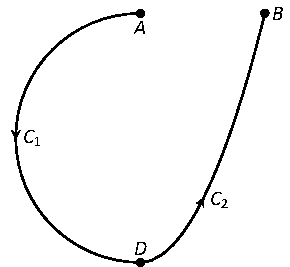
\includegraphics[width=0.25\textwidth]{fig_Vector_Calc_3a}}
\qquad
\subfigure[\label{fig_Vector_Calc_3b}]{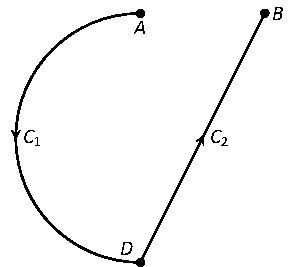
\includegraphics[width=0.25\textwidth]{fig_Vector_Calc_3b} }
\caption{Illustrating properties of line integrals.}
\end{figure}


\subsection{Centre of mass}
Let a curve $C$ (either in the plane or in space) represent a thin wire with variable density $\delta(s)$. We can approximate the mass of the wire by dividing the wire (i.e., the curve) into small segments of length $\Delta s_i$ and assume the density is constant across these small segments. The mass of each segment is density of the segment $\times$ its length; by summing up the approximate mass of each segment we can approximate the total mass:
$$\text{total mass of wire } \approx \sum\limits_i \delta(s_i)\Delta s_i.$$

By taking the limit as the length of the segments approaches 0, we have the definition of the line integral as seen in Definition \ref{def:line_integral1}. When learning of the line integral, we let $f(s)$ represent a height; now we let $f(s) = \delta(s)$ represent a density. We can extend this understanding of computing mass to also compute the centre of mass of a thin wire. We give the relevant formulas in the next definition, followed by an example.

\begin{definition}[Mass and centre of mass of a thin wire]\label{def:mass_of_thin_wire}
Let a thin wire lie along a smooth curve $C$ with continuous density function $\delta(s)$, where $s$ is the arc length parameter. 	\index{mass!centre of}\index[aut]{massamiddelpunt}\index{moment}\index[aut]{moment}%
\begin{enumerate}
	\item The \textbf{mass} (\textit{massa}) of the thin wire is $\ds M = \int_C \delta(s)\ ds$.
	\item The \textbf{moment about the $yz$-plane} is $\ds M_{yz} = \int_C x\delta(s)\ ds$.
	\item The \textbf{moment about the $xz$-plane} is $\ds M_{xz} = \int_C y\delta(s)\ ds$.
	\item The \textbf{moment about the $xy$-plane} is $\ds M_{xy} = \int_C z\delta(s)\ ds$.
	\item The \textbf{centre of mass} (\textit{massamiddelpunt}) of the wire is $$(\overline{x},\overline{y},\overline{z}) = \left(\frac{M_{yz}}M, \frac{M_{xz}}M,\frac{M_{xy}}M\right).$$
\end{enumerate}
\end{definition}

\begin{example}\label{ex_linescalarfield6}
A thin wire follows the path $\vrt = \left( 1+\cos(t),1+\sin(t), 1+ \sin(2t)\right)$, $0\leq t\leq 2\pi$. The density of the wire is determined by its position in space: $\delta(x,y,z) = y+z$ g/cm. The wire is shown in Figure \ref{fig_Vector_Calc_4}, where a light colour indicates low density and a dark colour represents high density. Find the mass  and centre of mass of the wire.


\begin{figure}[H]
	\begin{center}
			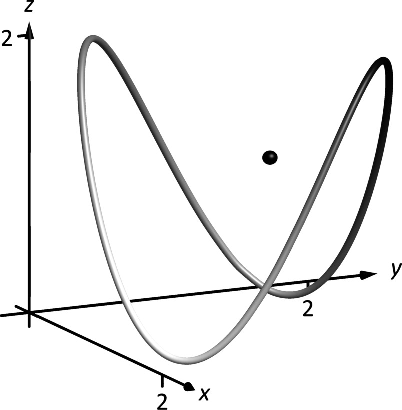
\includegraphics[width=0.38\textwidth]{fig_Vector_Calc_4}
	\caption{Finding the mass of a thin wire in Example \ref{ex_linescalarfield6}.}
	\label{fig_Vector_Calc_4}
	\end{center}
\end{figure}
\vspace*{-0.5cm}
\xhrulefill{gray}{2.5pt}Solution \xhrulefill{gray}{2.5pt}

We compute the density of the wire as 
$$\delta(x,y,z) = \delta\big(1+\cos(t),1+\sin(t), 1+\sin(2t)\big) = 2+\sin(t)+\sin(2t).$$ We compute $ds$ as
$$ds = \norm{\vrp(t)}\ dt = \sqrt{\sin^2(t)+\cos^2(t)+4\cos^2(2t)}\ dt = \sqrt{1+4\cos^2(2t)}\ dt.$$
Thus the mass is
$$M = \oint_C \delta(s)\ ds = \int\limits_0^{2\pi} \big(2+\sin(t)+\sin(2t)\big)\sqrt{1+4\cos^2(2t)}\ dt \approx 21.08 \text{ g }. $$
We compute the moments about the coordinate planes:%\small
\begin{align*}
M_{yz} &= \oint_C x\delta(s)\ ds = \int\limits_0^{2\pi}\big(1+\cos(t)\big)\big(2+\sin(t)+\sin(2t)\big)\sqrt{1+4\cos^2(2t)}\ dt \approx 21.08\, , \\
M_{xz} &= \oint_C y\delta(s)\ ds = \int\limits_0^{2\pi}\big(1+\sin(t)\big)\big(2+\sin(t)+\sin(2t)\big)\sqrt{1+4\cos^2(2t)}\ dt \approx
26.35\, ,\\
M_{xy} &= \oint_C z\delta(s)\ ds = \int\limits_0^{2\pi}\big(1+\sin(2 t)\big)\big(2+\sin(t)+\sin(2t)\big)\sqrt{1+4\cos^2(2t)}\ dt \approx 25.40.
\end{align*}%\normalsize
Thus the center of mass of the wire is located at 
$$(\overline{x},\overline{y},\overline{z}) = \left(\frac{M_{yz}}M, \frac{M_{xz}}M,\frac{M_{xy}}M\right) \approx (1,1.25,1.20),$$
as indicated by the dot in Figure \ref{fig_Vector_Calc_4}. Note how in this example, the curve $C$ is ''centered'' about the point $(1,1,1)$, though the variable density of the wire pulls the center of mass out along the $y$- and $z$-axes.
\end{example}


In the following, we investigate a new mathematical object, the vector field, after which we increase our understanding of integration in the context of vector fields.

\section{Vector fields}\label{sec:vector_fields}
\subsection{Definition}
	\checkoddpage
\marginpar{\ifoddpage\hspace*{-1.5cm}\else\hspace*{0.25cm}\fi
\includegraphics[width=0.075\textwidth]{youtube}\\
\ifoddpage\hspace*{-1.75cm}\else\hspace*{0.1cm}\fi
\qrcode[height=1.75cm]{https://youtu.be/gEa38ldV_a0}
%\includegraphics[width=0.1\textwidth]{fields}
}
We have studied functions, where the input of such functions is a point and the output is a number. We could also create functions where the input is a point, but the output is a  vector. For instance, we could create the following function: $\vec F(x,y) = \left( x+y, x-y\right)$, where $\vec F(2,3) = \left( 5,-1\right)$. We are to think of $\vec F$ assigning the vector $\left( 5,-1\right)$ to the point $(2,3)$; in some sense, the vector $\left( 5,-1\right)$ lies at the point $(2,3)$. 

Such functions are extremely useful in any context where magnitude and direction are important. For instance, we could create a function $\vec F$ that represents the electromagnetic force exerted at a point by a electromagnetic field, or the velocity of air as it moves across an airfoil. 

Because these functions are so important, we need to formally define them.

\begin{definition}[Vector field]\label{def:vector_field}
\begin{enumerate}
	\item A \textbf{vector field in the plane} (\textit{vectorveld in het vlak}) is a function $\vec F(x,y)$ whose domain is a subset of $\mathbb{R}^2$ and whose output is a two--dimensional vector:\index{vector field}
	$$\vec F(x,y) = \left( M(x,y), N(x,y)\right).$$
	
	\item A \textbf{vector field in $n$-dimensional space} (\textit{vectorveld in de $n$-dimensionale ruimte}) is a function $\vec F(\mathbf{x})$ whose domain is a subset of $\mathbb{R}^n$ and whose output is a $n$--dimensional vector:
	$$\vec F(\mathbf{x}) = \left( M_1(\mathbf{x}), M_2(\mathbf{x}),\ldots, M_n(\mathbf{x})\right).$$
\end{enumerate}
\end{definition}

This definition may seem odd at first, as a special type of function is called a field. However, as the function determines a field of vectors, we can say the field is defined by the function, and thus the field is a function.

 When graphing a vector field in the plane, the general idea is to draw the vector $\vec F(x,y)$ at the point $(x,y)$. For instance, using $\vec F(x,y) = \left( x+y,x-y\right)$ as before, at $(1,1)$ we would draw $\left( 2,0\right)$. 

In Figure \ref{fig_Vector_Calc_5a}, one can see that the vector $\left( 2,0\right)$ is drawn starting from the point $(1,1)$. A total of 8 vectors are drawn, with the $x$- and $y$-values of $-1,0,1$. In many ways, the resulting graph is a mess. In Figure \ref{fig_Vector_Calc_5b}, the same field is redrawn with each vector $\vec F(x,y)$ drawn centred on the point $(x,y)$. This makes for a better looking image, though when one vector intersects another, the image looks cluttered.

A common way to address this problem is limit the length of each arrow, and represent long vectors with thick arrows, as done in Figure \ref{fig_Vector_Calc_5c}. Usually we do not use a graph of a vector field to determine exactly the magnitude of a particular vector. Rather, we are more concerned with the relative magnitudes of vectors: which are bigger than others? Thus limiting the length of the vectors is not problematic.
\ifmathematica
Mathematica obviously allows us to plot many vectors in a vector field nicely; in Figure \ref{fig_Vector_Calc_5d}, we see the same vector field drawn with using the Mathematica command \lstinline{VectorPlot}, and finally get a clear picture of how this vector field behaves.\fi
\ifpython
Python obviously allows us to plot many vectors in a vector field nicely; in Figure \ref{fig_Vector_Calc_5d}, we see the same vector field drawn with using the Python command \lstinline{quiver}, and finally get a clear picture of how this vector field behaves.\fi
If this vector field represented the velocity of air moving across a flat surface, we could see that the air tends to move either to the upper--right or lower--left, and moves very slowly near the origin.  We can similarly plot vector fields in space, though the plots get very busy very quickly.


\begin{figure}[t]
\centering
%\raisebox{0.5cm}{
\subfigure[\label{fig_Vector_Calc_5a}]{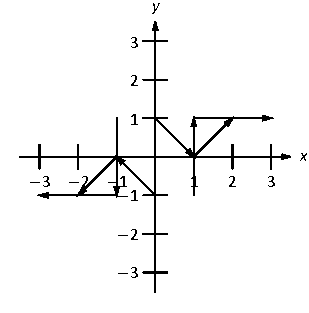
\includegraphics[width=0.43\textwidth]{fig_Vector_Calc_5a}}
\qquad
\subfigure[\label{fig_Vector_Calc_5b}]{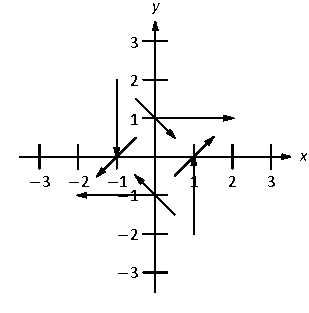
\includegraphics[width=0.43\textwidth]{fig_Vector_Calc_5b} }\\
\subfigure[\label{fig_Vector_Calc_5c}]{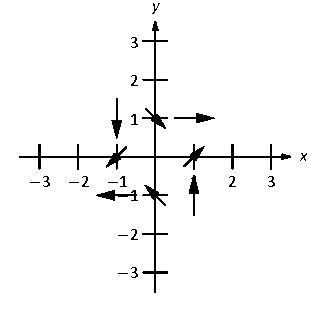
\includegraphics[width=0.43\textwidth]{fig_Vector_Calc_5c}}
\qquad
\subfigure[\label{fig_Vector_Calc_5d}]{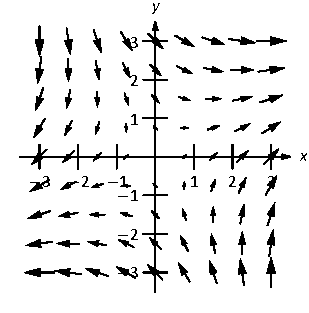
\includegraphics[width=0.43\textwidth]{fig_Vector_Calc_5d} }
\caption{Demonstrating methods of graphing vector fields.}
\end{figure}

\subsection{The del operator}
Often, we will drop the of $x$, $y$ and $z$ portions of the notation in Definition~\ref{def:vector_field} and refer to vector fields in the plane and in space as 
$$\vec F = \left( M, N\right) \quad \text{and} \quad \vec F  = \left( M,N,P\right),$$ respectively, as this shorthand is quite convenient.

Another item of notation will become useful: the del operator. \index{del operator}Recall in Section \ref{sec:directional_derivative} how we used the symbol $\vec{\nabla}$  to represent the gradient of a function of two variables. We now define $\vec{\nabla}$ to be the del operator. It is a vector whose components are partial derivative operations. 

In the plane, 
$$\ds\vec{\nabla} = \left( \frac{\partial}{\partial x}, \frac{\partial}{\partial y}\right);$$
in space, 
$$\ds\vec{\nabla} = \left( \frac{\partial}{\partial x}, \frac{\partial}{\partial y},\frac{\partial}{\partial z}\right).$$ 

With this definition of $\vec{\nabla}$, we can better understand the gradient $\vec{\nabla} f$. As $f$ returns a scalar, the properties of scalar and vector multiplication gives
$$\vec{\nabla} f = \left( \frac{\partial}{\partial x}, \frac{\partial}{\partial y}\right) f = \left( \frac{\partial}{\partial x}\,f, \frac{\partial}{\partial y}\,f\right) = \left( f_x, f_y\right).$$

Now apply the del operator $\vec{\nabla}$ to vector fields. Let $\vec F = \left( x+\sin(y),y^2+z,x^2\right)$. We can use vector operations and find the dot product of $\vec{\nabla}$ and $\vec F$:
\allowdisplaybreaks
\begin{align*}
\vec{\nabla} \cdot \vec F &=\left( \frac{\partial}{\partial x}, \frac{\partial}{\partial y},\frac{\partial}{\partial z}\right)\cdot  \left( x+\sin(y),y^2+z,x^2\right) \\
  &= \frac{\partial}{\partial x}\left(x+\sin(y)\right)+ \frac{\partial}{\partial y}\left(y^2+z\right) + \frac{\partial}{\partial z}\left(x^2\right) \\
		&=1+2y.
\end{align*}

We can also compute their cross products:
\allowdisplaybreaks
\begin{align*}
{\vec{\nabla}\times \vec F }&= {\left( \frac{\partial}{\partial y}\left(x^2\right)-\frac{\partial}{\partial z}\left(y^2+z\right),\frac{\partial}{\partial z}\left(x+\sin(y)\right)-\frac{\partial}{\partial x}\left(x^2\right),\frac{\partial}{\partial x}\left(y^2+z\right)-\frac{\partial}{\partial y}\left(x+\sin (y)\right)\right) }\\
&=\begin{vmatrix}\hat{i}&\hat{j}&\hat{k}\\[0.2cm]
\dfrac{\partial}{\partial x}&\dfrac{\partial}{\partial y}&\dfrac{\partial}{\partial z}\\[0.2cm]
x+\sin(y)&y^2+z&x^2\end{vmatrix}\\
&=\left( -1,-2x,-\cos(y)\right).
\end{align*}\normalsize

As we next learn about properties of vector fields, we will see how these dot and cross products with the del operator are quite useful.

\subsection{Divergence and curl}
	\checkoddpage
\marginpar{\ifoddpage\hspace*{-1.5cm}\else\hspace*{0.25cm}\fi
\includegraphics[width=0.075\textwidth]{youtube}\\
\ifoddpage\hspace*{-1.75cm}\else\hspace*{0.1cm}\fi
\qrcode[height=1.75cm]{https://youtu.be/c0MR-vWiUPU}
%\includegraphics[width=0.1\textwidth]{divergence}
}
Two properties of vector fields will prove themselves to be very important: divergence and curl. Each is a special ``derivative'' of a vector field; that is, each measures an instantaneous rate of change of a vector field.

If the vector field represents the velocity of a fluid or gas, then the divergence of the field is a measure of the compressibility of the fluid. If the divergence is negative at a point, it means that the fluid is compressing: more fluid is going into the point than is going out. If the divergence is positive, it means the fluid is expanding: more fluid is going out at that point than going in. A divergence of zero means the same amount of fluid is going in as is going out. If the divergence is zero at all points, we say the field is incompressible.

It turns out that the proper measure of divergence is simply $\vec{\nabla} \cdot \vec F$, as stated in the following definition.

\begin{definition}[Divergence]\label{def:divergence}
The \textbf{divergence of a vector field $\vec F$} (\textit{divergentie van een vectorveld}) is\index{divergence}\index[aut]{divergent}
$$\divv \vec F = \vec{\nabla} \cdot \vec F.$$
\begin{itemize}
	\item In the plane, with $\vec F = \left( M,N\right)$: \  $\divv \vec F = M_x+N_y$.
	\item In space, with $\vec F = \left( M,N,P\right)$: \  $\divv \vec F = M_x+N_y+P_z$.
\end{itemize}
\end{definition}

Curl is a measure of the spinning action of the field. Let $\vec F$ represent the flow of water over a flat surface. If a small round cork were held in place at a point in the water, would the water cause the cork to spin? No spin corresponds to zero curl; counterclockwise spin corresponds to positive curl and clockwise spin corresponds to negative curl. 

In space, things are a bit more complicated. Again let $\vec F$ represent the flow of water, and imagine suspending a tennis ball in one location in this flow. The water may cause the ball to spin along an axis. If so, the curl of the vector field is a vector (not a scalar, as before), parallel to the axis of rotation, following a right hand rule: when the thumb of one's right hand points in the direction of the curl, the ball will spin in the direction of the curling fingers of the hand.

In space, it turns out the proper measure of curl is $\vec{\nabla} \times \vec F$, as stated in the following definition. To find the curl of a planar vector field $\vec F = \left( M,N\right)$, embed it into space as $\vec F = \left( M, N, 0\right)$ and apply the cross product definition. Since $M$ and $N$ are functions of just $x$ and $y$ (and not $z$), all partial derivatives with respect to $z$ become 0 and the result is simply $\left( 0,0,N_x-M_y\right)$. The third component is the measure of curl of a planar vector field. 

\begin{definition}[Curl]\label{def:curl}
\begin{itemize}
	\item Let $\vec F = \left( M,N\right)$ be a vector field in the plane. The \textbf{curl of $\vec F$} (\textit{rotatie of rotor van $\vec F$}) is $$\curl \vec F = N_x - M_y.$$\index{curl}\index[aut]{rotatie}
	\item Let $\vec F = \left( M,N,P\right)$ be a vector field in space. The \textbf{curl of $\vec F$} (\textit{rotatie of rotor van $\vec F$}) is $$\curl \vec F = \vec{\nabla} \times \vec F = \left( P_y-N_z,\,M_z-P_x,\,N_x - M_y\right).$$
\end{itemize}
\end{definition}

We adopt the convention of referring to curl as $\vec{\nabla} \times \vec F$, regardless of whether $\vec F$ is a vector field in two or three dimensions. 

We now practice computing these quantities.

\begin{example}\label{ex_vectorfield1}
For each of the planar vector fields given below, view its graph and try to visually determine if its divergence and curl are 0. Then compute the divergence and curl.

\begin{multicols}{2}
\begin{enumerate}
	\item $\vec F = \left( y,0\right)$\quad  (see Figure \ref{fig_Vector_Calc_6a})
	\item $\vec F = \left( -y,x\right)$ \quad  (see Figure \ref{fig_Vector_Calc_6b})
	\item $\vec F = \left( x,y\right)$ \quad  (see Figure \ref{fig_Vector_Calc_6c})
	\item $\vec F = \left( \cos(y), \sin(x)\right)$ \quad  (see Figure \ref{fig_Vector_Calc_6d})
\end{enumerate}
\end{multicols}




\xhrulefill{gray}{2.5pt}Solution \xhrulefill{gray}{2.5pt}


\begin{enumerate}
	\item The arrow sizes are constant along any horizontal line, so if one were to draw a small box anywhere on the graph, it would seem that the same amount of fluid would enter the box as exit. Therefore it seems the divergence is zero; it is, as 
	$$\divv\vec F = \vec{\nabla} \cdot \vec F = M_x + N_y = \frac{\partial}{\partial x}(y) + \frac{\partial}{\partial y}(0) = 0.$$

	At any point on the $x$-axis, arrows above it move to the right and arrows below it move to the left, indicating that a cork placed on the axis would spin clockwise. A cork placed anywhere above the $x$-axis would have water above it moving to the right faster than the water below it, also creating a clockwise spin. A clockwise spin also appears to be created at points below the $x$-axis. Thus it seems the curl should be negative (and not zero). Indeed, it is:
	$$\curl \vec F = \vec{\nabla}\times\vec F = N_x-M_y = \frac{\partial}{\partial x}(0) - \frac{\partial}{\partial y}(y) = -1.$$
	
	\item It appears that all vectors that lie on a circle of radius $r$, centered at the  origin, have the same length (and indeed this is true). That implies that the divergence should be zero: draw any box on the graph, and any fluid coming in will lie along a circle that takes the same amount of fluid out. Indeed, the divergence is zero, as
	$$\divv\vec F = \vec{\nabla} \cdot \vec F = M_x + N_y = \frac{\partial}{\partial x}(-y) + \frac{\partial}{\partial y}(x) = 0.$$
	
\begin{figure}[H]
\centering
%\raisebox{0.5cm}{
\subfigure[\label{fig_Vector_Calc_6a}]{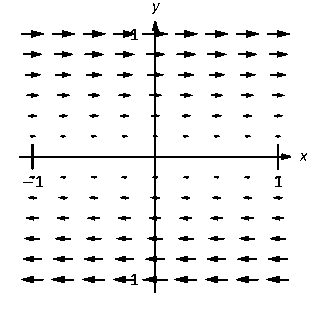
\includegraphics[width=0.4\textwidth]{fig_Vector_Calc_6a}}
\qquad
\subfigure[\label{fig_Vector_Calc_6b}]{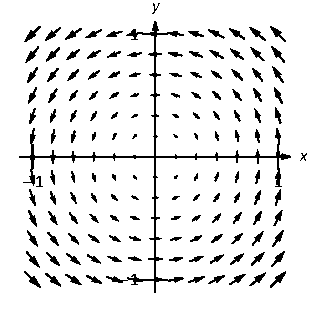
\includegraphics[width=0.4\textwidth]{fig_Vector_Calc_6b} }\\
\subfigure[\label{fig_Vector_Calc_6c}]{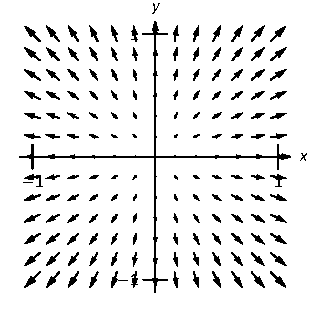
\includegraphics[width=0.4\textwidth]{fig_Vector_Calc_6c}}
\qquad
\subfigure[\label{fig_Vector_Calc_6d}]{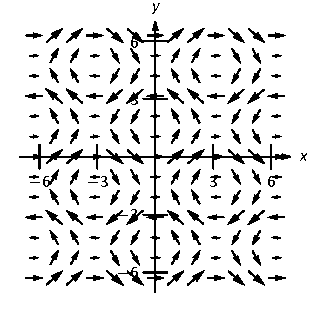
\includegraphics[width=0.4\textwidth]{fig_Vector_Calc_6d} }
\caption{The vector fields in parts 1 (a), 2 (b), 3 (c) and 4 (d) in Example \ref{ex_vectorfield1}.}
\end{figure}

		Clearly this field moves objects in a circle, but would it induce a cork to spin? It appears that yes, it would: place a cork anywhere in the flow, and the point of the cork closest to the origin would feel less flow than the point on the cork farthest from the origin, which would induce a counterclockwise flow. Indeed, the curl is positive:
	$$\curl \vec F = \vec{\nabla}\times\vec F = N_x-M_y = \frac{\partial}{\partial x}(x) - \frac{\partial}{\partial y}(-y) = 1-(-1) = 2.$$
	Since the curl is constant, we conclude the induced spin is the same no matter where one is in this field.
	
	\item At the origin, there are many arrows pointing out but no arrows pointing in. We conclude that at the origin, the divergence must be positive (and not zero). If one were to draw a box anywhere in the field, the edges farther from the origin would have larger arrows passing through them than the edges close to the origin, indicating that more is going from a point than going in. This indicates a positive (and not zero) divergence. This is correct:
	$$\divv\vec F = \vec{\nabla} \cdot \vec F = M_x + N_y = \frac{\partial}{\partial x}(x) + \frac{\partial}{\partial y}(y) = 1+1=2.$$
	
	One may find this curl to be harder to determine visually than previous examples. One might note that any arrow that induces a clockwise spin on a cork will have an equally sized arrow inducing a counterclockwise spin on the other side, indicating no spin and no curl. This is correct, as
	$$\curl \vec F = \vec{\nabla}\times\vec F = N_x-M_y = \frac{\partial}{\partial x}(y) - \frac{\partial}{\partial y}(x) = 0.$$
	

	\item	One might find this divergence hard to determine visually as large arrows appear in close proximity to small arrows, each pointing in different directions. Instead of trying to rationalize a guess, we compute the divergence:
	$$\divv\vec F = \vec{\nabla} \cdot \vec F = M_x + N_y = \frac{\partial}{\partial x}\left(\cos(y)\right) + \frac{\partial}{\partial y}\left(\sin(x)\right) = 0.$$ 
	Perhaps surprisingly, the divergence is 0.
	
	With all the loops of different directions in the field, one is apt to reason the curl is variable. Indeed, it is:
	$$\curl \vec F = \vec{\nabla}\times\vec F = N_x-M_y = \frac{\partial}{\partial x}\left(\sin(x)\right) - \frac{\partial}{\partial y}\left(\cos(y)\right) = \cos(x) + \sin(y).$$
	Depending on the values of $x$ and $y$, the curl may be positive, negative, or zero.
\end{enumerate}



\end{example}


\begin{example}\label{ex_vectorfield3}
The force of gravity between two objects is inversely proportional to the square of the distance between the objects. Locate a point mass at the origin. Create a vector field $\vec F$ that represents the gravitational pull of the point mass at any point $(x,y,z)$. Find the divergence and curl of this field. 


\xhrulefill{gray}{2.5pt}Solution \xhrulefill{gray}{2.5pt}

The point mass pulls toward the origin, so at $(x,y,z)$, the force will pull in the direction of $\left( -x, -y, -z\right)$. To get the proper magnitude, it will be useful to find the unit vector in this direction. Dividing by its magnitude, we have $$\vec u = \left( \frac{-x}{\sqrt{x^2+y^2+z^2}}, \frac{-y}{\sqrt{x^2+y^2+z^2}},\frac{-z}{\sqrt{x^2+y^2+z^2}}\right).$$
The magnitude of the force is inversely proportional to the square of the distance between the two points. Letting $k$ be the constant of proportionality, we have the magnitude as $$\ds\frac{k}{x^2+y^2+z^2}.$$ Multiplying this magnitude by the unit vector above, we have the desired vector field:
$$\vec F = \left( \frac{-kx}{(x^2+y^2+z^2)^{3/2}}, \frac{-ky}{(x^2+y^2+z^2)^{3/2}},\frac{-kz}{(x^2+y^2+z^2)^{3/2}}\right).$$
We leave it to the reader to confirm that $\divv \vec F = 0$ and $\curl \vec F = \vec 0$.

The analogous planar vector field is given in Figure \ref{fig_Vector_Calc_7}. Note how all arrows point to the origin, and the magnitude gets very small when far from the origin.

\begin{figure}[H]
	\begin{center}
			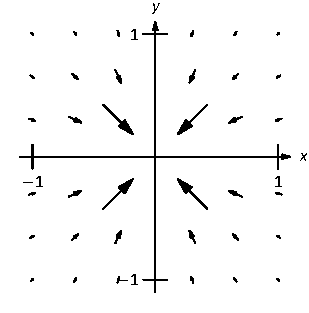
\includegraphics[width=0.5\textwidth]{fig_Vector_Calc_7}
	\caption{A vector field representing a planar gravitational force.}
	\label{fig_Vector_Calc_7}
	\end{center}
\end{figure}

\end{example}




A function $z=f(x,y)$ naturally induces a vector field, $\vec F = \vec{\nabla} f = \left( f_x,f_y\right)$. Given what we learned of the gradient in Section \ref{sec:directional_derivative}, we know that the vectors of $\vec F$ point in the direction of greatest increase of $f$. Because of this, $f$ is said to be the \textbf{potential function of} $\vec F$. Vector fields that are the gradient of potential functions will play an important role in the remainder of this  section.

The last part of this section applies calculus to vector fields. A common application is this: let $\vec F$ be a vector field representing a force (hence it is called a force field) and let a particle move along a curve $C$ under the influence of this force. What work is performed by the field on this particle? The solution lies in correctly applying the concepts of line integrals in the context of vector fields.

\section{Line Integrals over vector fields}\label{sec:line_int_vf}
\subsection{Definition}
Suppose a particle moves along a curve $C$ under the influence of an electromagnetic force described by a vector field $\vec F$. Since a force is inducing motion, work is performed. How can we calculate how much work is performed?

Recall that when moving in a straight line, if $\vec F$ represents a constant force and $\vec d$ represents the direction and length of travel, then work is simply $W = \vec F\cdot \vec d$. However, we generally want to be able to calculate work even if $\vec F$ is not constant and $C$ is not a straight line.

As we have practised many times before, we can calculate work by first approximating, then refining our approximation through a limit that leads to integration. 

Assume as we did at the beginning of this section, $C$ can be parametrized by the arc length parameter $s$. Over a short piece of the curve with length $ds$, the curve is approximately straight and our force is approximately constant. The straight--line direction of this short length of curve is given by $\widehat T$, the unit tangent vector;   let $\vec d = \widehat T\,ds$, which gives  the direction and magnitude of a small section of $C$. Thus work over this small section of $C$ is $\vec F \cdot \vec d = \vec F\cdot \widehat T\, ds$. 

Summing up all the work over these small segments gives an approximation of the work performed. By taking the limit as $ds$ goes to zero, and hence the number of segments approaches infinity, we can obtain the exact amount of work. Hence, we see that 
$$W = \int_C \vec F\cdot \widehat T\,ds,$$
is a line integral.

This line integral is beautiful in its simplicity, yet is not so useful in making actual computations (largely because the arc length parameter is so difficult to work with). To compute actual work, we need to parametrize $C$ with another parameter $t$ via a vector--valued function $\vec r(t)$. Since $ds = \norm{\vrp(t)}\,dt$ and $\widehat T = \vrp(t)/\norm{\vrp(t)}$, we get
\begin{equation}
W = \int_C \vec F\cdot\widehat T\ ds = \int_C \vec F\cdot \frac{\vrp(t)}{\norm{\vrp(t)}}\ \norm{\vrp(t)}\ dt = \int_C\vec F\cdot \vrp(t)\ dt = \int_C \vec F\cdot d\vec r,
\label{eq:line_integral}\end{equation}
where the final integral uses the differential $d\vec r$ for $\vrp(t)\,dt$.

These integrals are known as line integrals over vector fields. By contrast, the line integrals we dealt with earlier are sometimes referred to as line integrals over scalar fields (Definition~\ref{def:line_integral1}). Just as a vector field is defined by a function that returns a vector, a scalar field is a function that returns a scalar, such as $z = f(x,y)$.

We formally define this line integral, then give examples and applications.

\begin{definition}[Line integral over a vector field]\label{def:line_integral2}
Let $\vec F$ be a vector field with continuous components defined on a smooth curve $C$, parametrized by $\vrt$, and let $\widehat T$ be the unit tangent vector of $\vrt$. The \textbf{line integral over $\vec F$} along $C$ is\index{line integral}
$$\int_C \vec F\cdot d\vec r = \int_C \vec F\cdot\widehat T\ ds.$$
\end{definition}

In Definition \ref{def:line_integral2}, note how the dot product $\vec F \cdot \widehat T$ is just a scalar. 
Therefore, this new line integral is really just a special kind of line integral. Indeed, letting $f(s) = \vec F(s)\cdot \widehat T(s)$, the right--hand side simply becomes $\int_C f(s)\ ds$, and we can use the corresponding techniques to evaluate the integral. This is summarized in the following theorem. 

\begin{theorem}[Evaluating a line integral over a vector field]\label{idea:line2}
Let $\vec F$ be a vector field with continuous components defined on a smooth curve $C$, parametrized by $\vrt$, $a\leq t\leq b$, where $\vec r$ is continuously differentiable. Then\index{vector field!over vector field}
	$$\int_C\vec F\cdot\widehat T\ ds = \int_C \vec F\cdot d\vec r =\int\limits_a^b \vec F\big(\vec r(t)\big) \cdot \vrp(t)\ dt.$$
\end{theorem}

This theorem indicates that we can use any continuously differentiable parametrization $\vrt$ of $C$ that preserves the orientation of $C$: there isn't a right one. In practice, choose one that seems easy to work with. 

Note that the above definition and theorem implicitly evaluate $\vec F$ along the curve $C$, which is parametrized by $\vrt$. For instance, if $\vec F = \left( x+y, x-y\right)$ and $\vrt = \left( t^2,\cos(t)\right)$, then evaluating $\vec F$ along $C$ means substituting the $x$- and $y$-components of $\vrt$ in for $x$ and $y$, respectively, in $\vec F$. Therefore, along $C$, $\vec F = \left( x+y,x-y\right) = \left( t^2+\cos(t), t^2-\cos(t)\right)$. Since we are substituting the output of $\vrt$ for the input of $\vec F$, we write this as $\vec F\big(\vrt\big)$. This is a slight abuse of notation as technically the input of $\vec F$ is to be a point, not a vector, but this shorthand is useful.


\begin{example}\label{ex_livf1}
Two particles move from $(0,0)$ to $(1,1)$ under the influence of the force field $\vec F  = \left( x, x+y\right)$. One particle follows $C_1$, the line $y=x$; the other follows $C_2$, the curve $y=x^4$, as shown in Figure \ref{fig_Vector_Calc_8}. Force is measured in Newtons and distance is measured in meters. Find the work performed by each particle.


\begin{figure}[H]
	\begin{center}
			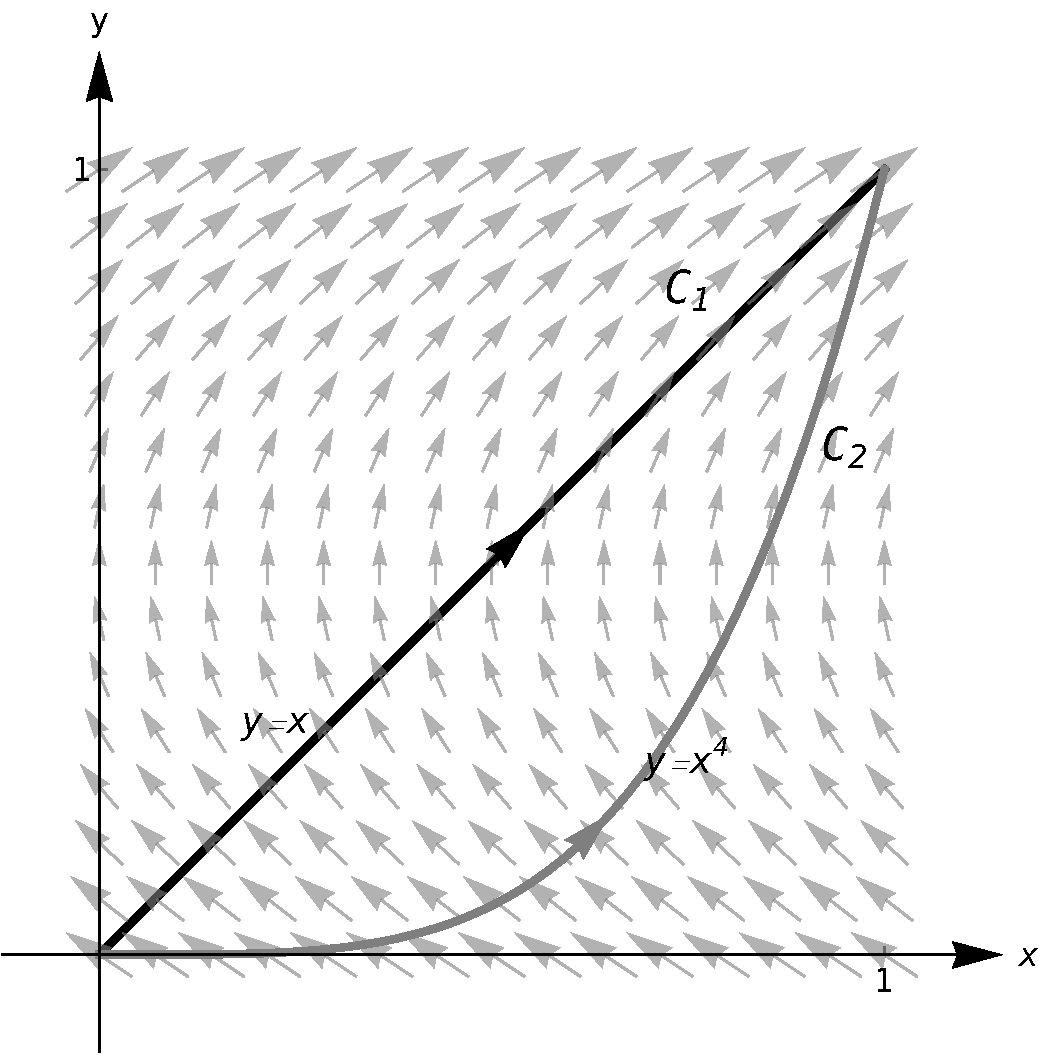
\includegraphics[width=0.5\textwidth]{fig_Vector_Calc_8}
	\caption{Paths through a vector field in Example \ref{ex_livf1}.}
	\label{fig_Vector_Calc_8}
	\end{center}
\end{figure}


\xhrulefill{gray}{2.5pt}Solution \xhrulefill{gray}{2.5pt}

To compute work, we need to parametrize each path. We use $\vec r_1(t) = \left( t,t\right)$ to parametrize $y=x$, and let $\vec r_2(t) =\left( t,t^4\right)$ parametrize $y=x^4$; for each, $0\leq t\leq 1$. 

Along the straight--line path, $\vec F\big(\vec r_1(t)\big) = \left( x, x+y\right) = \left( t, t+t\right) = \left( t,2t\right)$. We find $\vrp_1(t) =\left( 1,1\right)$. The integral that computes work is:
\begin{align*}
\int_{C_1} \vec F\cdot d\vec r &= \int\limits_0^1 \left( t,2t\right)\cdot\left( 1,1\right)\ dt \\
			&= \int\limits_0^1 3t\ dt \\
			&= \left(\frac32t^2\right)\Bigg|_0^1 = 1.5 \text{ joules}.
\end{align*}

Along the curve $y = x^4$, we have that
$$\vec F\big(\vec r_2(t)\big) = \left( x, x+y\right) = \left( t, t+t^4\right).$$ We find $\vrp_2(t) = \left( 1,4t^3\right)$. The work performed along this path is
\begin{align*}
\int_{C_2} \vec F\cdot d\vec r &= \int\limits_0^1 \left( t,t+t^4\right)\cdot\left( 1,4t^3\right)\ dt\\
			&= \int\limits_0^1 \big(t + 4t^4+ 4t^7\big)\ dt \\
			&= \left(\frac12t^2 + \frac45t^5 + \frac12t^8\right)\Bigg|_0^1 =  \frac95 \text{ joules}.
\end{align*}


Note how differing amounts of work are performed along the different paths. This should not be too surprising: the force is variable, one path is longer than the other, etc.
\end{example}

\begin{example}\label{ex_livf2}
Two particles move from $(-1,1)$ to $(1,1)$ under the influence of a force field $\vec F = \left( y, x\right)$. One moves along the curve $C_1$, the parabola defined by $y = 2x^2-1$. The other particle moves along the curve $C_2$, the bottom half of the circle defined by $x^2+(y-1)^2=1$, as shown in Figure \ref{fig_Vector_Calc_9}. Force is measured in Newton and distances are measured in meters. Find the work performed by moving each particle along its path.

\begin{figure}[H]
	\begin{center}
			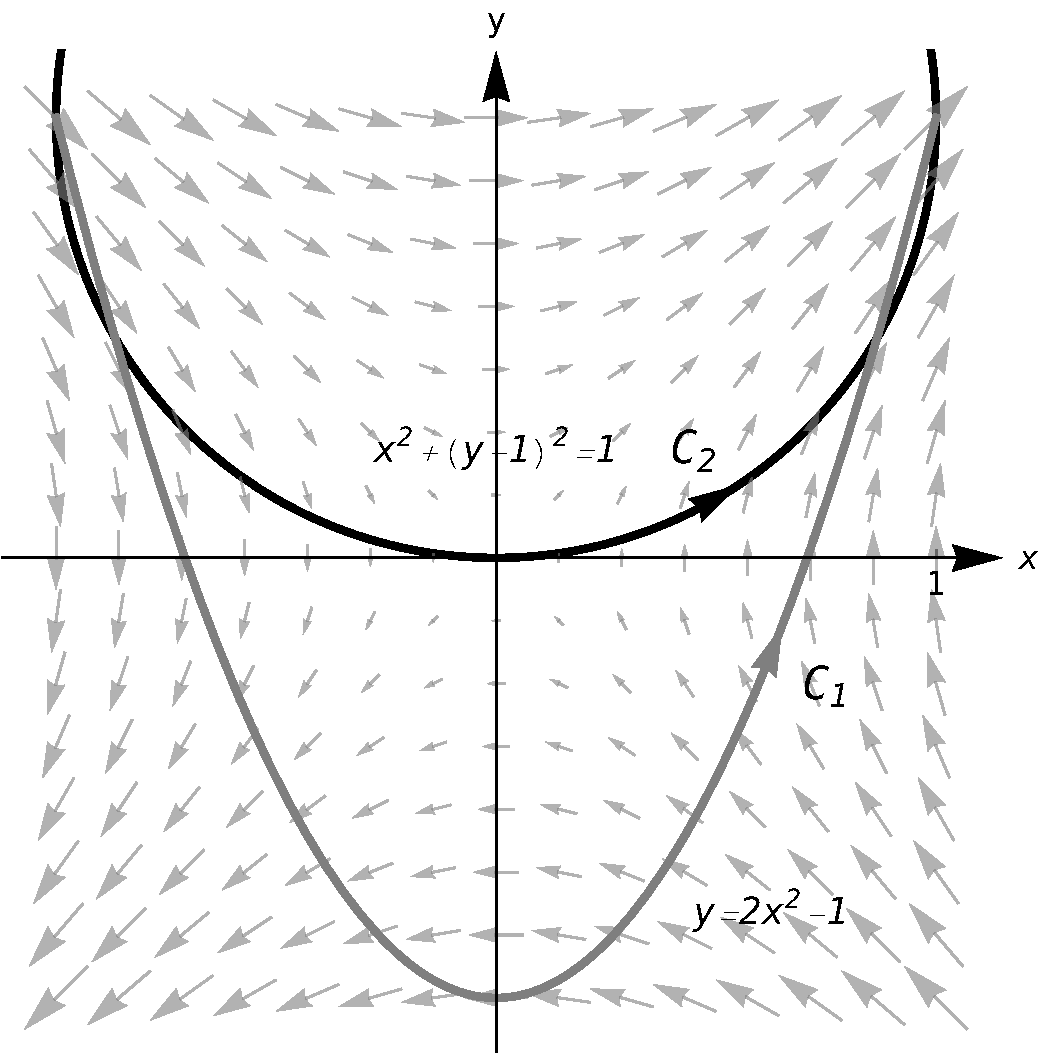
\includegraphics[width=0.5\textwidth]{fig_Vector_Calc_9}
	\caption{Paths through a vector field in Example \ref{ex_livf2}.}
	\label{fig_Vector_Calc_9}
	\end{center}
\end{figure}


\xhrulefill{gray}{2.5pt}Solution \xhrulefill{gray}{2.5pt}

We start by parametrizing $C_1$: the parametrization $\vec r_1(t) = \left( t, 2t^2-1\right)$ is straightforward, giving $\vrp_1 = \left( 1,4t\right)$. On $C_1$, $\vec F\big(\vec r_1(t)\big) = \left( y,x\right) = \left( 2t^2-1,t\right)$.


Computing the work along $C_1$, we have:
\begin{align*}
\int_{C_1} \vec F\cdot d\vec r_1 & = \int\limits_{-1}^1 \left( 2t^2-1,t\right)\cdot\left( 1,4t\right)\ dt \\
		&= \int\limits_{-1}^1 \big(2t^2-1+4t^2\big)\ dt = 2 \text{ joules}.
\end{align*}





For $C_2$, it is probably simplest to parametrize the half circle using sine and cosine. Recall that $\vec r(t) = \left( \cos(t), \sin(t)\right)$ is a parametrization of the unit circle on $0\leq t\leq 2\pi$; we add 1 to the second component to shift the circle up one unit, then restrict the domain to $\pi\leq t\leq 2\pi$  to obtain only the lower half, giving $\vec r_2(t) = \left( \cos(t), \sin(t)+1\right)$, $\pi\leq t\leq 2\pi$, and hence $\vrp_2(t) = \left( -\sin(t), \cos(t)\right)$ and $\vec F\big(\vec r_2(t)\big) = \left(y,x\right) = \left( \sin(t)+1,\cos(t)\right)$.


Computing the work along $C_2$, we have:
\begin{align*}
\int_{C_2} \vec F\cdot d\vec r_2 & = \int\limits_{\pi}^{2\pi} \left( \sin(t)+1,\cos(t)\right)\cdot\left( -\sin(t),\cos(t)\right)\ dt \\
		&= \int\limits_{\pi}^{2\pi} \big(-\sin^2(t)-\sin(t)+\cos^2(t)\big)\ dt = 2 \text{ joules}.
\end{align*}
Note how the work along $C_1$ and $C_2$ in this example is the same. 
\end{example}

\subsection{Properties}
Line integrals over vector fields share the same properties as line integrals over scalar fields, with one important distinction. The orientation of the curve $C$ matters with line integrals over vector fields, whereas it did not matter with line integrals over scalar fields.

It is relatively easy to see why. Let $C$ be the unit circle. The area under a surface over $C$ is the same whether we traverse the circle in a clockwise or counterclockwise fashion, hence the line integral over a scalar field on $C$ is the same irrespective of orientation. On the other hand, if we are computing work done by a force field, direction of travel definitely matters. Opposite directions create opposite signs when computing dot products, so traversing the circle in opposite directions will create line integrals that differ by a factor of $-1$. 

In summary, we have the following properties of line integrals over vector fields. 

\begin{enumerate}
	\item	Let $\vec F$ and $\vec G$ be  vector fields with continuous components defined on a smooth curve $C$, parametrized by $\vrt$, and let $k_1$ and $k_2$ be scalars. Then\index{line integral!properties over a vector field}
	$$\ds \int_C\big(k_1\vec F+k_2\vec G\big)\cdot d\vec r = k_1\int_C\vec F\cdot d\vec r +k_2\int_C\vec G\cdot d\vec r.$$
	\item Let $C$ be piecewise smooth, composed of smooth components $C_1$ and $C_2$. Then
	$$\int_C\vec F\cdot d\vec r = \int_{C_1}\vec F\cdot d\vec r + \int_{C_2}\vec F\cdot d\vec r.$$
	\item	Let $C^*$ be the curve $C$ with opposite orientation, parametrized by $\vec r^*$. Then
	$$\int_C\vec F\cdot d\vec r = -\int_{C^*}\vec F\cdot d\vec r^*.$$
	\end{enumerate}

We demonstrate using these properties in the following example.

\begin{example}\label{ex_livf3}
Let $\vec F = \left( 3(y-1/2),1\right)$ and let $C$ be the path that starts at $(0,0)$, goes to $(1,1)$ along the curve $y=x^3$, then returns to $(0,0)$ along the line $y=x$, as shown in Figure \ref{fig_Vector_Calc_10}. Evaluate $\oint_C \vec F\cdot d\vec r$.


\begin{figure}[H]
	\begin{center}
			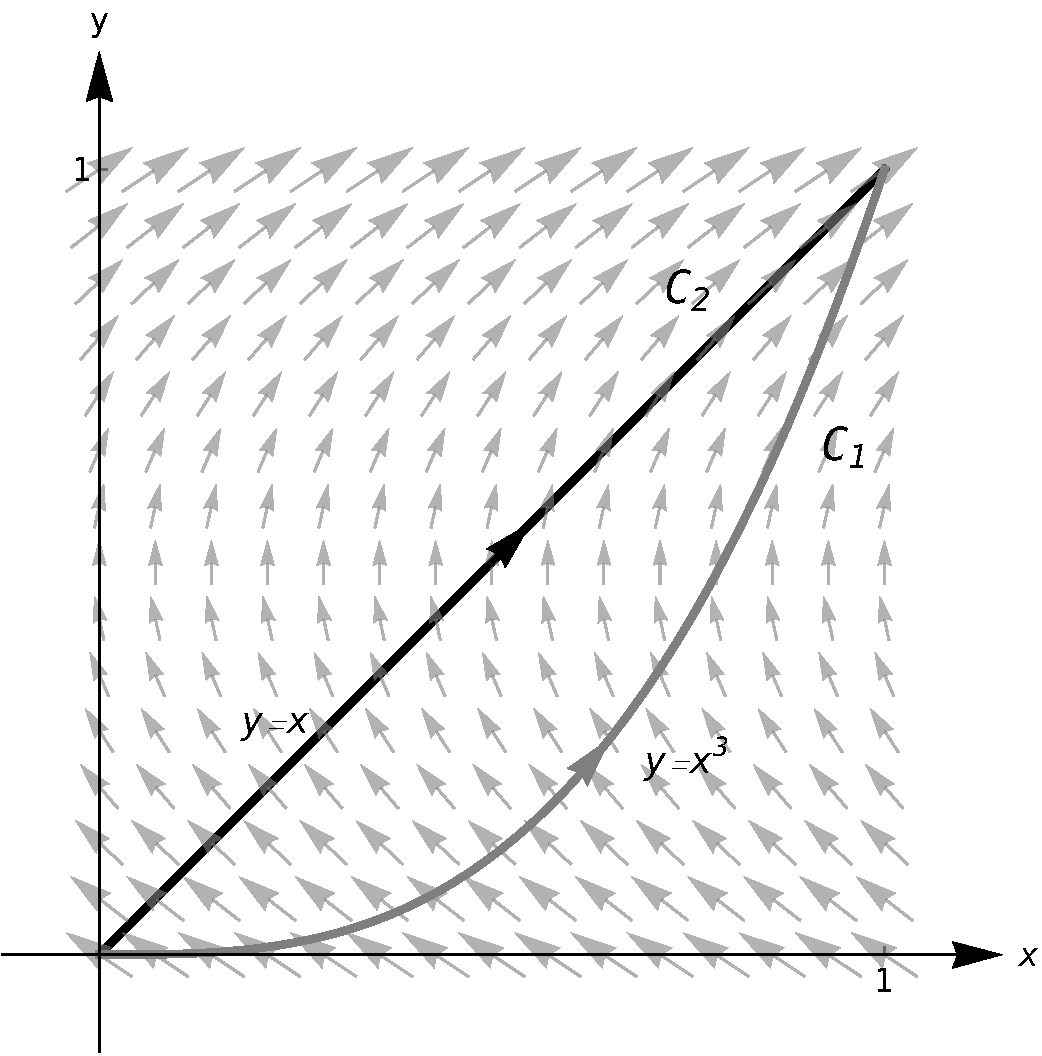
\includegraphics[width=0.5\textwidth]{fig_Vector_Calc_10}
	\caption{The vector field and curve in Example \ref{ex_livf3}.}
	\label{fig_Vector_Calc_10}
	\end{center}
\end{figure}


\xhrulefill{gray}{2.5pt}Solution \xhrulefill{gray}{2.5pt}

As $C$ is piecewise smooth, we break it into two components $C_1$ and $C_2$, where $C_1$ follows the curve $y=x^3$ and $C_2$ follows the curve $y=x$. 

We parametrize $C_1$ with $\vec r_1(t) = \left( t, t^3\right)$ on $0\leq t\leq 1$, with $\vrp_1(t) = \left( 1,3t^2\right)$. We will use \linebreak $\vec F\big(\vec r_1(t)\big) = \left( 3(t^3-1/2),1\right)$.

While we always have unlimited ways in which to parametrize a curve, there are two direct methods to choose from when parametrizing $C_2$. The parametrization $\vec r_2(t)=\left( t,t\right)$, $0\leq t\leq 1$ traces the correct line segment but with the wrong orientation. Relying on property (3) of line integrals over vector fields, we can use this parametrization and negate the result.

Another choice is to use the techniques of Section \ref{sec:lines} to create the line with the orientation we desire. We wish to start at $( 1,1)$ and travel in the $\vec d = \left( -1,-1\right)$ direction for one length of $\vec d$, giving equation $\vec \ell(t) = \left( 1,1\right) + t\left( -1,-1\right) = \left( 1-t,1-t\right)$ on $0\leq t\leq 1$.

Either choice is fine; we choose $\vec r_2(t)$ to practice using line integral properties. We find \linebreak $\vrp_2(t) = \left( 1,1\right)$ and $\vec F\big(\vec r_2(t)\big) = \left( 3(t-1/2),1\right)$.

Evaluating the line integral:
\begin{align*}
\oint_C \vec F\cdot d\vec r &= \int_{C_1}\vec F\cdot d\vec r_1 - \int_{C_2}\vec F\cdot d\vec r_2 \\
			&= \int\limits_0^1 \left( 3\left(t^3-\dfrac{1}{2}\right),1\right)\cdot \left( 1,3t^2\right) dt- \int\limits_0^1 \left( 3\left(t-\dfrac{1}{2}\right),1\right)\cdot \left(1,1\right) dt \\
			&= \int\limits_0^1\left(3t^3+3t^2-\dfrac{3}{2}\right)\ dt - \int\limits_0^1 \left(3t-\dfrac{1}{2}\right)\ dt\\
			&= \dfrac{1}{4} - 1 = -\dfrac{3}{4}.
\end{align*}
If we interpret this integral as computing work, the negative work implies that the motion is mostly against the direction of the force, which seems plausible when we look at Figure \ref{fig_Vector_Calc_10}.
\end{example}

\subsection{The fundamental theorem of line integrals}

	\checkoddpage
\marginpar{\ifoddpage\hspace*{-1.5cm}\else\hspace*{0.25cm}\fi
\includegraphics[width=0.075\textwidth]{youtube}\\
\ifoddpage\hspace*{-1.75cm}\else\hspace*{0.1cm}\fi
\qrcode[height=1.75cm]{https://youtu.be/6S3BJSsc72Q}
%\includegraphics[width=0.1\textwidth]{regions}
}
We are preparing to make important statements about the value of certain line integrals over special vector fields. Before we can do that, we need to define some terms that describe the domains over which a vector field is defined.

A region in the plane is \textbf{connected}\index{connected}\index[aut]{samenhangend} (\textit{samenhangend}) if any two points in the region can be joined by a piecewise smooth curve that lies entirely in the region. In Figure \ref{fig_Vector_Calc_11a}, sets $R_1$ and $R_2$ are connected; set $R_3$ is not connected, though it is composed of two connected subregions.

A region is \textbf{simply connected} (\textit{enkelvoudig samenhangend})\index{simply connected}\index{connected!simply}\index[aut]{samenhangend ! enkelvoudig} if every simple closed curve that lies entirely in the region can be continuously deformed (shrunk) to a single point without leaving the region.  (A curve is \textbf{simple}\index{simple curve} if it does not cross itself.) In Figure \ref{fig_Vector_Calc_11a}, only set $R_1$ is simply connected. Region $R_2$ is not simply connected as any closed curve that goes around the ``hole'' in $R_2$ cannot be continously shrunk to a single point. As $R_3$ is not even connected, it cannot be simply connected, though again it consists of two simply connected subregions. 

We have applied these terms to regions of the plane, but they can be extended intuitively to domains in space (and hyperspace). In Figure \ref{fig_Vector_Calc_11b}, the domain bounded by the sphere (at left) and the domain with a subsphere removed (at right) are both simply connected. Any simple closed path that lies entirely within these domains can be continuously deformed into a single point. In Figure \ref{fig_Vector_Calc_11c}, neither domain is simply connected. At left, the ball has a hole that extends its length and the pictured closed path cannot be deformed to a point. At right, two paths are illustrated on the torus that cannot be shrunk to a point. 

We will use the terms connected and simply connected in subsequent definitions and theorems.

\begin{figure}
\centering
%\raisebox{0.5cm}{
\subfigure[\label{fig_Vector_Calc_11a}]{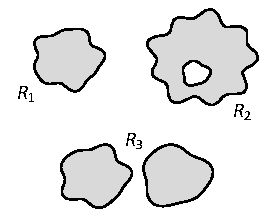
\includegraphics[width=0.43\textwidth]{fig_Vector_Calc_11a}}
\qquad
\subfigure[\label{fig_Vector_Calc_11b}]{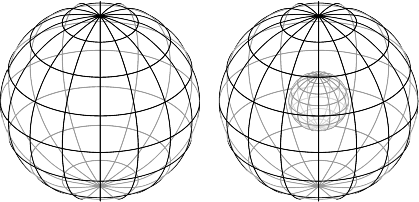
\includegraphics[width=0.43\textwidth]{fig_Vector_Calc_11b} }\\

\subfigure[\label{fig_Vector_Calc_11c}]{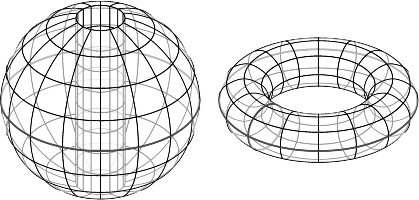
\includegraphics[width=0.43\textwidth]{fig_Vector_Calc_11c}}
\caption{Different types of regions (a): $R_1$ is simply connected; $R_2$ is connected, but not simply connected; $R_3$ is not connected; simply connected domains (b) and not simply connected domains in (c).}
\end{figure}

Recall how in Example \ref{ex_livf2} particles moved from $A = (-1,1)$ to $B = (1,1)$ along two different paths, wherein the same amount of work was performed along each path. It turns out that regardless of the choice of path from $A$ to $B$, the amount of work performed under the field $\vec F = \left( y, x\right)$ is the same. Since our expectation is that differing amounts of work are performed along different paths, we give such special fields a name. 

\pagebreak
\begin{definition}[Conservative field]\label{def:conservative}
Let $\vec F$ be a vector field defined on an open, connected domain $D$ containing points $A$ and $B$. If the line integral
$\int_C \vec F\cdot d\vec r$\ \ has the same value for all choices of paths $C$ starting at $A$ and ending at $B$, and parametrized by $\vec{r}(t)$,  then\index{conservative field}\index{vector field!conservative}\index{path independent}\index{line integral!path independent}\index[aut]{vectorveld!conservatief}\index[aut]{vectorveld!exact}\index[aut]{conservatief vectorveld}
\begin{itemize}
	\item $\vec F$ is a \textbf{conservative field} (\textit{conservatief vectorveld}) and
	\item	The line integral $\int_C \vec F\cdot d\vec r$ is path independent and can be written as $$\int_C \vec F\cdot d\vec r = \int\limits_A^B \vec F\cdot \ d\vec r.$$ 
\end{itemize}
\end{definition}


How can we tell if a field is conservative? To show a field $\vec F$ is conservative using the definition, we need to show that all line integrals from points $A$ to $B$ have the same value. It is equivalent to show that all line integrals over closed paths $C$ are 0. Each of these tasks are generally nontrivial.

There is, however, a simpler method. Consider the surface defined by $z = f(x,y) = xy$. We can compute the gradient of this function: $\vec{\nabla} f = \left( f_x, f_y\right) = \left( y, x\right)$. Note that this is the field from Example \ref{ex_livf2}, which we have claimed is conservative. We will soon give a theorem that states that a field $\vec F$ is conservative if, and only if, it is the gradient of some scalar function $f$. To show $\vec F$ is conservative, we need to determine whether or not $\vec F = \vec{\nabla} f$ for some function $f$. To recognize the special relationship between $\vec F$ and $f$ in this situation, $f$ is given a name.

\begin{definition}[Potential function]\label{def:potential}
Let $f$ be a differentiable function defined on a  domain $D$  (e.g., $z = f(x,y)$ or $w = f(x,y,z)$) and let $\vec F = \vec{\nabla} f$, the gradient of $f$. Then $f$ is a \textbf{potential function} (\textit{potentiaalfunctie}) of $\vec F$.\index{potential function}\index{vector field!potential function}\index[aut]{vectorveld!potentiaalfunctie}\index[aut]{potentiaalfunctie}
\end{definition}

We now state the fundamental theorem of line integrals, also known as the gradient theorem, which connects conservative fields and path independence to fields with potential functions. 

\begin{theorem}[Fundamental theorem of line integrals]\label{thm:FTofLineIntegrals}
Let $\vec F$ be a vector field whose components are continuous on a connected domain $D$, let $A$ and $B$ be any points in $D$, and let $C$ be any path in $D$ starting at $A$ at $t=a$,  ending at $B$ at $t=b$ and parametrized by $\vec{r}(t)$ such that $\vec{r}(a)=A$ and  $\vec{r}(b)=B$. 
\begin{enumerate}
	\item $\vec F$ is conservative if and only if there exists a differentiable function $f$ such that $\vec F = \vec{\nabla} f$. 
	\item	If $\vec F$ is conservative, then 
	$$\int_C\vec F\cdot d\vec r = \int\limits_A^B \vec F\cdot d\vec r =f\left( {\vec r\left( b \right)} \right) - f\left( {\vec r\left( a \right)} \right)= f(B) - f(A).$$
\end{enumerate}
\end{theorem}

Note that we did not specify the number of variables for the function since it is really immaterial to the theorem. The theorem will hold regardless of the number of variables in the function.


\ifanalysis
\begin{proof}
For the purpose of the proof we will assume that we are working in three dimensions, but it can be done in any dimension. Let us then start by just computing the line integral.
\begin{align*}
\int_C{{\vec{\nabla} f\cdot d\vec r}} & = \int\limits_{{\,a}}^{{\,b}}{{\vec{\nabla} f\left( {\vec r\left( t \right)} \right)\cdot \vec r'\left( t \right)\,dt}}\\ &  = \int\limits_{{\,a}}^{{\,b}}{{\left( {\frac{{\partial f}}{{\partial x}}\frac{{dx}}{{dt}} + \frac{{\partial f}}{{\partial y}}\frac{{dy}}{{dt}} + \frac{{\partial f}}{{\partial z}}\frac{{dz}}{{dt}}} \right)\,dt}}
\end{align*}

Now, at this point we can use the chain rule to simplify the integrand as follows,
\begin{align*}\int_C{{\vec{\nabla} f\cdot d\vec r}} & = \int\limits_{{\,a}}^{{\,b}}{{\left( {\frac{{\partial f}}{{\partial x}}\frac{{dx}}{{dt}} + \frac{{\partial f}}{{\partial y}}\frac{{dy}}{{dt}} + \frac{{\partial f}}{{\partial z}}\frac{{dz}}{{dt}}} \right)\,dt}}\\ &  = \int\limits_{{\,a}}^{{\,b}}{{\frac{d}{{dt}}\left[ {f\left( {\vec r\left( t \right)} \right)} \right]\,dt}}
\end{align*}

To finish this off we just need to use the fundamental theorem of calculus for single integrals.
$$
\int_C{{\vec{\nabla} f\cdot d\vec r}} = f\left( {\vec r\left( b \right)} \right) - f\left( {\vec r\left( a \right)} \right)=f(B)-f(A)
$$
%Bron: 
%http://tutorial.math.lamar.edu/Classes/CalcIII/FundThmLineIntegrals.aspx
\end{proof}
\fi

Once again considering Example \ref{ex_livf2}, we have $A = (-1,1)$, $B = (1,1)$ and $\vec F = \left( y,x\right)$. In that example, we evaluated two line integrals from $A$ to $B$ and found the value of each was 2. Note that $f(x,y) = xy$ is a potential function for $\vec F$. Following the fundamental theorem of line integrals, consider $f(B) - f(A)$:
$$f(B) - f(A) = f(1,1) - f(-1,1) = 1 - (-1) = 2,$$
the same value given by the line integrals.


We practice using this theorem again in the next example.

\begin{example}\label{ex_livf5}
Let $\vec F = \left( 3x^2y+2x, x^3+1\right)$, $A = (0,1)$ and $B = (1,4)$. Use the first part of the fundamental theorem of line integrals to show that $\vec F$ is conservative, then choose any path from $A$ to $B$ and confirm the second part of the theorem.

\xhrulefill{gray}{2.5pt}Solution \xhrulefill{gray}{2.5pt}


To show $\vec F$ is conservative, we need to find $z = f(x,y)$ such that $\vec F = \vec{\nabla} f = \left( f_x, f_y\right)$. That is, we need to find $f$ such that $f_x = 3x^2y+2x$ and $f_y = x^3+1$. As all we know about $f$ are its partial derivatives, we recover $f$ by integration:
$$\int\limits \frac{\partial f}{\partial x}\ dx = f(x,y) + K_1(y).$$
Note how the constant of integration $K_1(y)$ is more than just a constant: it is anything that acts as a constant when taking a derivative with respect to $x$. Any function that is a function of $y$ (containing no $x$'s) acts as a constant when deriving with respect to $x$.

Integrating $f_x$ in this example gives:
$$\int\limits \frac{\partial f}{\partial x}\ dx = \int\limits (3x^2y+2x)\ dx = x^3y+x^2 + K_1(y).$$

Likewise, integrating $f_y$ with respect to $y$ gives:
$$\int\limits \frac{\partial f}{\partial y}\ dy = \int\limits( x^3+1)\ dy = x^3y+ y + K_2(x).$$

These two results should be equal with appropriate choices of $K_2(x)$ and $K_1(y)$:
$$x^3y+x^2 + K_1(y) = x^3y+ y + K_2(x)\quad \Rightarrow\quad K_2(x) = x^2 \quad \text{and}\quad K_1(y) = y.$$

We find $f(x,y) = x^3y+x^2+y$, a potential function of $\vec F$. 

By the fundamental theorem of line integrals, regardless of the path from $A$ to $B$, 
\begin{align*}
\int\limits_A^B\vec F\cdot d\vec r &= f(B) - f(A) \\[-0.3cm]
			&= f(1,4) - f(0,1) \\
			&= 9 - 1 = 8.
\end{align*}
To illustrate the validity of the Fundamental Theorem, we pick a path from $A$ to $B$. The line between these two points would be simple to construct; we choose a slightly more complicated path by choosing the parabola $y = x^2+2x+1$. This leads to the parametrization $\vrt = \left( t, t^2+2t+1\right)$, $0\leq t\leq 1$, with $\vrp(t) = \left( 1, 2t+2\right)$. Thus
\begin{align*}
\int_C \vec F\cdot d\vec r &= \int_C\vec F\big(\vrt\big)\cdot\vrp(t)\ dt\\
				&= \int\limits_0^1\left( 3t^2(t^2+2t+1)+2t, t^3+1\right)\cdot\left( 1,2t+2\right)\ dt\\
				&= \int\limits_0^1 \left(5t^4+8t^3+3t^2+4t+2\right)\ dt\\
				&= \left(t^5+2t^4+t^3+2t^2+2t\right)\Big|_0^1\\
				&= 8,
\end{align*}				
which matches our previous result.
\end{example}

The fundamental theorem of line integrals states that we can determine whether or not $\vec F$ is conservative by determining whether or not $\vec F$ has a potential function. This can be difficult. A simpler method exists if the domain of $\vec F$ is simply connected, which is a reasonable requirement. We state this simpler method as a theorem.


\begin{theorem}[Curl of conservative fields]\label{thm:conservative_field_curl}
Let $\vec F$ be a vector field whose components are continuous on a simply connected domain $D$ in the plane or in space. Then $\vec F$ is conservative if and only if $\curl \vec F = 0$ or $\vec 0$, respectively.
\end{theorem}

In Example \ref{ex_livf5}, we showed that $\vec F =\left( 3x^2y+2x,x^3+1\right)$ is conservative by finding a potential function for $\vec F$. Using the above theorem, we can show that $\vec F(M,N)$ is conservative much more easily by computing its curl:
$$\curl \vec F = N_x - M_y = 3x^2 - 3x^2 = 0.$$





\section{Green's theorem and the divergence theorem}
\label{sec:greensthm}
\subsection{Flow and flux}
Line integrals over vector fields have the natural interpretation of computing work when $\vec F$ represents a force field. It is also common to use vector fields to represent velocities. In these cases, the line integral $\int_C \vec F\cdot d\vec r$ is said to represent \textbf{flow} (\textit{stroming}).\index{flow}\index{flux}\index{circulation}




Let the vector field $\vec F = \left( 1,0\right)$ represent the velocity of water as it moves across a smooth surface, depicted in Figure \ref{fig_Vector_Calc_12}. A line integral over $C$ will compute how much water is moving \textit{along} the path $C$.


\begin{figure}
	\begin{center}
			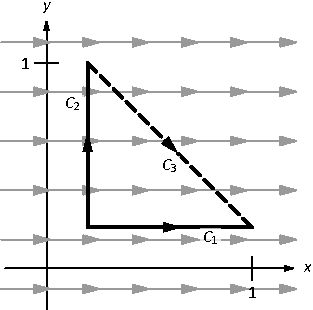
\includegraphics[width=0.5\textwidth]{fig_Vector_Calc_12}
	\caption{Illustrating the principles of flow and flux.}
	\label{fig_Vector_Calc_12}
	\end{center}
\end{figure}


In the figure, all of the water above $C_1$ is moving along that curve, whereas none of the water above $C_2$ is moving along that curve (the curve and the flow of water are at right angles to each other). Because $C_3$ has nonzero horizontal and vertical components, some of the water above that curve is moving along the curve.

	\checkoddpage
\marginpar{\ifoddpage\hspace*{-1.5cm}\else\hspace*{0.25cm}\fi
\includegraphics[width=0.075\textwidth]{youtube}\\
\ifoddpage\hspace*{-1.75cm}\else\hspace*{0.1cm}\fi
\qrcode[height=1.75cm]{https://youtu.be/e_XUFkSMaYk}
%\includegraphics[width=0.1\textwidth]{circulatie}
}
When $C$ is a closed curve, we call flow \textbf{circulation} (\textit{circulatie}), represented by $\oint_C \vec F\cdot d\vec r$.

The opposite of flow is \textbf{flux}, a measure of how much water is moving \textit{across} the path $C$. If a curve represents a filter in flowing water, flux measures how much water will pass through the filter. Considering again Figure \ref{fig_Vector_Calc_12}, we see that a screen along $C_1$ will not filter any water as no water passes across that curve. Because of the nature of this field,  $C_2$ and $C_3$ each filter the same amount of water per second. 

	\checkoddpage
\marginpar{\ifoddpage\hspace*{-1.5cm}\else\hspace*{0.25cm}\fi
\includegraphics[width=0.075\textwidth]{youtube}\\
\ifoddpage\hspace*{-1.75cm}\else\hspace*{0.1cm}\fi
\qrcode[height=1.75cm]{https://youtu.be/mEI7ACWmx_8}
%\includegraphics[width=0.1\textwidth]{flux_2d}
}
The terms flow and flux are used apart from velocity fields, too. Flow is measured by $\int_C \vec F\cdot d\vec r$, which is the same as $\int_C \vec F\cdot\widehat T\ ds$ by Definition \ref{def:line_integral2}. That is, flow is a summation of the amount of $\vec F$ that is tangent to the curve $C$. 

By contrast, flux is a summation of the amount of $\vec F$ that is \textit{orthogonal} to the direction of travel. To capture this orthogonal amount of $\vec F$, we use $\int_C \vec F \cdot \hat n\ ds$ to measure flux, where $\hat n$ is a unit vector orthogonal to the curve $C$. 

How is $\hat n$ determined? We'll later see that if $C$ is a closed curve, we'll want $\hat n$ to point to the outside of the curve (measuring how much is going out). We'll also adopt the convention that closed curves should be traversed counterclockwise. 

If $C$ is a complicated closed curve, it can be difficult to determine what counterclockwise means.  So we offer this definition: a closed curve is being traversed counterclockwise if the outside is to the right of the path and the inside is to the left.

When a curve $C$ is traversed counterclockwise by $\vrt = \left( f(t), g(t)\right)$, we rotate $\widehat T$ clockwise 90$^\circ$  to obtain $\hat n$:
$$\widehat T =\frac{\vec{r}'(t)}{\norm{\vrp(t)}}= \frac{\left( \fp(t),g'(t)\right)}{\norm{\vrp(t)}} \quad \Rightarrow \quad \hat n = \frac{\left( g'(t),-\fp(t)\right)}{\norm{\vrp(t)}}.$$

Letting $\vec F = \left( M, N\right)$, we calculate flux as:
\allowdisplaybreaks
\begin{align*}
\int_C \vec F\cdot \hat n\ ds &= \int_C \vec F\cdot \frac{\left( g'(t),-\fp(t)\right)}{\norm{\vrp(t)}} \ \norm{\vrp(t)}\ dt \\
				&= \int_C \left( M, N\right) \cdot \left( g'(t),-\fp(t)\right)\ dt \\
				&= \int_C \left(M\,g'(t) - N\,\fp(t)\right)\ dt\\
				&= \int_C M\,g'(t)\ dt - \int_C N\,\fp(t)\ dt.\\
				\intertext{As the $x$- and $y$-components of $\vrt$ are $f(t)$ and $g(t)$ respectively, the differentials of $x$ and $y$ are $dx = \fp(t)\ dt$ and $dy=g'(t)\ dt$. We can then write the above integrals as:}\\
			\int_C \vec F\cdot \hat n\ ds 	&= \int_C M\ dy - \int_C N\ dx.\\
				\intertext{The right-hand side is often written as one integral (not incorrectly, though somewhat confusingly, as this one integral has two ``$d$\,'s''):}
			\int_C \vec F\cdot \hat n\ ds 	&=\int_C \big( M\ dy -N\ dx \big)\,.
\end{align*}
We summarize the above in the following definition.

\begin{definition}[Flow, flux]
\label{def:flowflux}
Let $\vec F=\left( M(x,y),N(x,y)\right)$ be a vector field with continuous components defined on a smooth curve $C$, parametrized by $\vrt =\left( f(t),g(t)\right)$, let $\widehat T$ be the unit tangent vector of $\vrt$, and let $\hat n$ be the clockwise 90$^\circ$ rotation of $\widehat T$.\index{flow}\index{flux}
\begin{itemize}
	\item The \textbf{flow} (\textit{stroming}) of $\vec F$ along $C$ is
$$\int_C \vec F\cdot\widehat T\ ds=\int_C \vec F\cdot d\vec r.$$
	\item The \textbf{flux} (\textit{flux}) of $\vec F$ across $C$ is
$$\int_C \vec F\cdot \hat n\ ds =  \int_C \big( M\ dy -N\ dx \big)= \int_C\left(M\,g'(t) - N\,\fp(t)\right)\ dt. $$
\end{itemize}
\end{definition}

This definition of flow also holds for curves in space, though it does not make sense to measure flux across a curve in space. Measuring flow is essentially the same as finding work performed by a force as done in the previous examples. Therefore we practice finding only flux in the following example.

\begin{example}
\label{ex_flux1}
Curves $C_1$ and $C_2$ each start at $(1,0)$ and end at $(0,1)$, where $C_1$ follows the line $y=1-x$ and $C_2$ follows the unit circle, as shown in Figure \ref{fig_Vector_Calc_13a}. Find the flux across both curves for the vector fields $\vec F_1 = \left( y, -x+1\right)$ and $\vec F_2 = \left( -x, 2y-x\right)$. 





\xhrulefill{gray}{2.5pt}Solution \xhrulefill{gray}{2.5pt}


We begin by finding parametrizations of $C_1$ and $C_2$. As done in Example \ref{ex_livf3}, parametrize $C_1$ by creating the line that starts at $(1,0)$ and moves in the $\left( -1,1\right)$ direction: \\ $\vec r_1(t) = \left( 1,0\right) + t\left( -1,1\right) = \left( 1-t, t\right)$, for $0\leq t\leq 1$. We parametrize $C_2$ with the familiar \\ $\vec r_2(t) = \left( \cos (t),\sin (t) \right)$ on $0\leq t\leq \pi/2$. For reference later, we give each function and its derivative below:
$$ \vec r_1(t) = \left( 1-t, t\right), \quad \vrp_1(t) = \left( -1,1\right).$$
$$\vec r_2(t) = \left( \cos (t), \sin (t)\right), \quad \vrp_2(t) = \left( -\sin (t) ,\cos (t)\right).$$

When $ \vec F_1 = \left( y, -x+1\right)$ (as shown in Figure \ref{fig_Vector_Calc_13a}), over $C_1$ we have $M = y =t$ and \\ $N = -x+1 = -(1-t)+1 = t$. Using Definition \ref{def:flowflux}, we compute the flux:
\begin{align*}
\int_{C_1} \vec F_1\cdot \hat n\ ds & = \int_{C_1} \left(M\,g'(t) - N\,\fp(t)\right)\ dt\\
			&= \int\limits_0^1 \left( t(1) - t(-1)\right)\ dt \\
			&= \int\limits_0^1 2t\ dt\\
			&= 1.
\end{align*}
Over $C_2$, we have $M = y = \sin (t)$ and $N = -x+1 = 1-\cos (t)$. Thus the flux across $C_2$ is:
\begin{align*}
\int_{C_2} \vec F_1\cdot \hat n\ ds & = \int_{C_2} \left(M\,g'(t) - N\,\fp(t)\right)\ dt\\
				&= \int\limits_0^{\pi/2}\left( \sin (t)\cos (t) - (1-\cos (t))(-\sin (t))\right)\ dt\\
				&= \int\limits_0^{\pi/2} \sin (t)\ dt\\
				&=1.
\end{align*}
Notice how the flux was the same across both curves. This won't hold true when we change the vector field.


When $ \vec F_2 = \left( -x,2y-x\right)$ (as shown in Figure \ref{fig_Vector_Calc_13b}), over $C_1$ we have $M = -x = t-1$ and $N = 2y-x = 2t-(1-t) = 3t-1$. Computing the flux across $C_1$:
\begin{align*}
\int_{C_1} \vec F_2\cdot \hat n\ ds & = \int_{C_1} \left(M\,g'(t) - N\,\fp(t)\right)\ dt\\
			&= \int\limits_0^1 \left( (t-1)(1) - (3t-1)(-1)\right)\ dt \\
			&= \int\limits_0^1 \left(4t-2\right)\ dt\\
			&= 0.
\end{align*}
Over $C_2$, we have $M = -x = -\cos (t)$ and $N = 2y-x = 2\sin (t)-\cos (t)$. Thus the flux across $C_2$ is:
\begin{align*}
\int_{C_2} \vec F_2\cdot \hat n\ ds & = \int_{C_2} \left(M\,g'(t) - N\,\fp(t)\right)\ dt\\
				&= \int\limits_0^{\pi/2}\left( -\cos (t)\cos (t) - (2\sin t-\cos (t))(-\sin (t))\right)\ dt\\
				&= \int\limits_0^{\pi/2} \left(2\sin^2 (t)-\sin (t)\cos t-\cos^2(t)\right)\ dt\\
				&=\dfrac{\pi}{4} - \dfrac{1}{2}\approx 0.285.
\end{align*}
\begin{figure}[H]
\centering
%\raisebox{0.5cm}{
\subfigure[\label{fig_Vector_Calc_13a}]{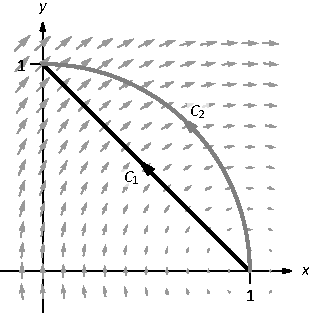
\includegraphics[width=0.43\textwidth]{fig_Vector_Calc_13a}}
\qquad
\subfigure[\label{fig_Vector_Calc_13b}]{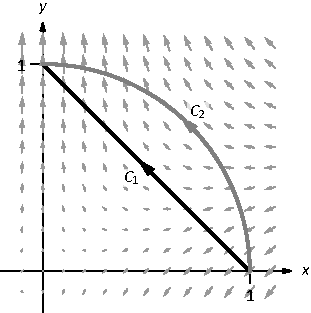
\includegraphics[width=0.43\textwidth]{fig_Vector_Calc_13b} }
\caption{Illustrating the curves and vector fields in Example \ref{ex_flux1}. In (a) the vector field is $\vec F_1$, and in (b) the vector field is $\vec F_2$.}
\end{figure}
We analyse the results of this example below.
\end{example}



In Example \ref{ex_flux1}, we saw that the flux across the two curves was the same when the vector field was $\vec F_1 = \left( y, -x+1\right)$. This is not a coincidence. We show why they are equal in Example \ref{ex_div2}. In short, the reason is this: the divergence of $\vec F_1$ is 0, and when $\divv \vec F = 0$, the flux across any two paths with common beginning and ending points will be the same.

We also saw in the example that the flux across $C_1$ was 0 when the field was $\vec F_2 = \left( -x, 2y-x\right)$. Flux measures ``how much'' of the field crosses the path from left to right (following the conventions established before). Positive flux means most of the field is crossing from left to right; negative flux means most of the field is crossing from right to left; zero flux means the same amount crosses from each side. When we consider Figure \ref{fig_Vector_Calc_13b}, it seems plausible that the same amount of $\vec F_2$ was crossing $C_1$ from left to right as from right to left.




\subsection{Green's theorem}

	\checkoddpage
\marginpar{\ifoddpage\hspace*{-1.5cm}\else\hspace*{0.25cm}\fi
\includegraphics[width=0.075\textwidth]{youtube}\\
\ifoddpage\hspace*{-1.75cm}\else\hspace*{0.1cm}\fi
\qrcode[height=1.75cm]{https://youtu.be/8SwKD5_VL5o}
%\includegraphics[width=0.1\textwidth]{green}
}
There is an important connection between the circulation around a closed region $R$ and the curl of the vector field inside of $R$, as well as a connection between the flux across the boundary of $R$ and the divergence of the field inside $R$. These connections are described by Green's theorem and the divergence theorem, respectively. We will explore each in turn.

Green's theorem states ``the counterclockwise circulation around a closed region $R$ is equal to the sum of the curls over $R$.''

\pagebreak
\begin{theorem}[Green's theorem]
\label{thm:greens}
Let $R$ be a closed, bounded region of the plane whose boundary $C$ is composed of finitely many smooth curves, let $\vec r(t)$ be a counterclockwise parametrization of $C$, and let $\vec F =\left( M,N\right)$ where $N_x$ and $M_y$ are continuous over $R$. Then\index{Green's theorem}
$$\oint_C \vec F\cdot d\vec r = \iint_R\curl \vec F\ dA= \iint_R\left(N_x-M_y\right) \ dA.$$
\end{theorem}

\begin{proof}

It suffices to demonstrate the theorem for rectangular regions in the $xy$-plane. The Riemann sum nature of the double integral will then guarantee the proof of the theorem for arbitrary regions, because a Riemann sum is technically a summation of the areas of arbitrarily small rectangles. As the proof is for a rectangle, the proof will work for arbitrary regions, which can be approximated by collections of ever smaller rectangles. 

First of all, let us recall that $\vec F =\left( M,N\right)$ and that $d\vec r =(dx,dy)$, such that we can rewrite the contour integral as
$$
\oint_C \big(M\ dx + N\ dy\big)\,. 
$$


Let $R=\left\{(x,y)\left|\, a\leq x\leq b,c\leq y\leq d \right. \right\}$ be a rectangular region, and let the boundary $C$ of $R$ be oriented counterclockwise. We break this boundary into four pieces (Figure~\ref{fig_Vector_Calc_14}):
\begin{enumerate}
\item $C_1$, which runs from $(a,c)$ to $(b,c)$\,,  
\item $C_2$, which runs from $(b,c)$ to $(b,d)$\,, 
\item  $C_3$, which runs from $(b,d)$ to $(a,d)$\,, 
\item $C_4$, which runs from $(a,d)$ to $(a,c)$.
\end{enumerate}


\begin{figure}
	\begin{center}
			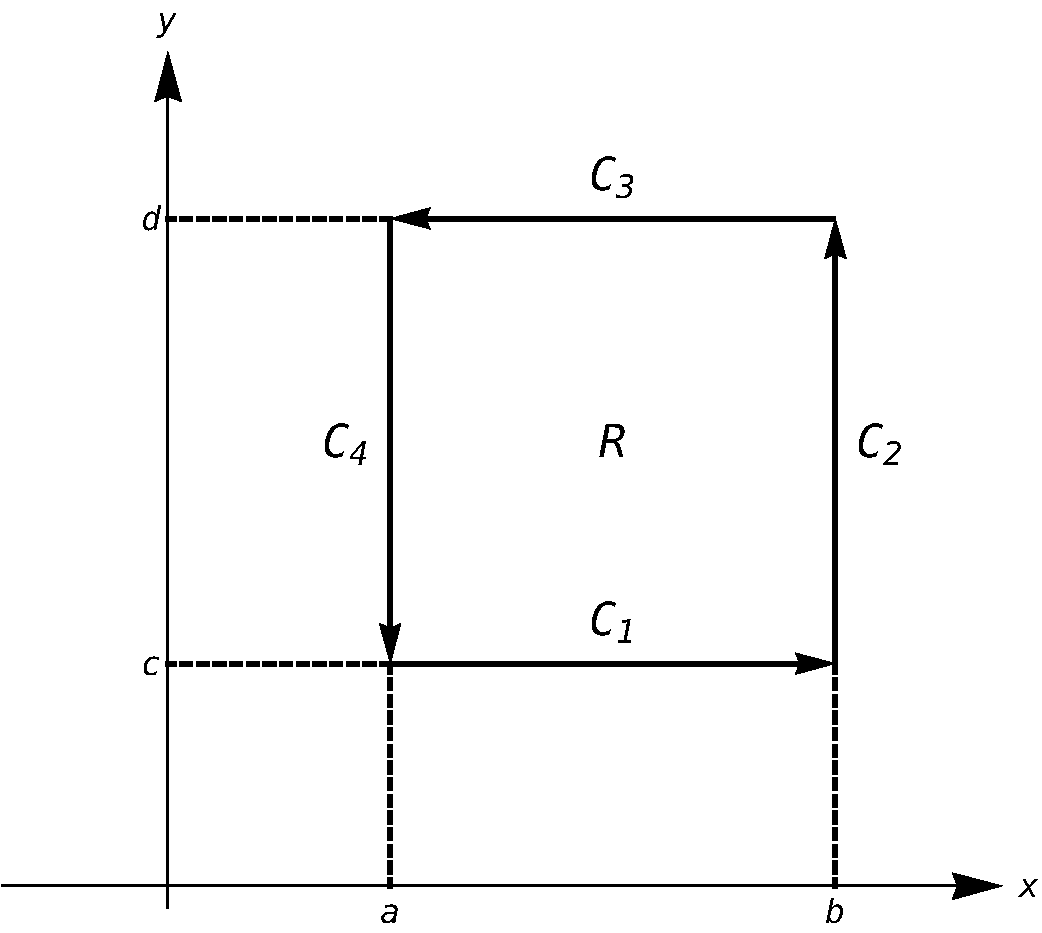
\includegraphics[width=0.4\textwidth]{fig_Vector_Calc_14}
	\caption{The rectangular region used in the proof of Green's theorem.}
	\label{fig_Vector_Calc_14}
	\end{center}
\end{figure}


Then,
\begin{eqnarray*}
\displaystyle \iint_R \frac{\partial N}{\partial x} \ dx\ dy &=&  \int\limits_c^d \int\limits_a^b \frac {\partial N} {\partial x}\ dx\ dy \\[0.2cm]
&=& \int\limits_c^d \left({N \left({b, y}\right) - N \left({a, y}\right) }\right) \ dy\\
&=&\int\limits_c^d  N \left({b, y}\right)\ dy+ \int\limits_d^c N \left({a, y}\right)\ dy\\[0.2cm]
&=& \int_{C_2} N \ dy+ \int_{C_4} N\ dy\,.
\end{eqnarray*}
We note that $y$ is constant along $C_1$ and $C_3$, so
$$
\displaystyle \int_{C_1} N \ dy = \int_{C_3} N \ dy = 0\,.
$$ 
Hence
\begin{eqnarray*}
\displaystyle \iint_R \frac{\partial N}{\partial x} \ dx\ dy =\displaystyle \int_{C_2} N\ dy + \int_{C_4} N \ dy&=&\displaystyle \int_{C_1} N \ dy + \int_{C_2} N \ dy + \int_{C_3} N \ dy + \int_{C_4} N \ dy\\[0.2cm]
&=&\oint_C N\ dy\,.
\end{eqnarray*}
A similar argument demonstrates that: 
$$
\displaystyle \iint_R \frac{\partial M}{\partial y} \ dy \ dx = - \oint_C M \ dx\,.
$$

Consequently, we have that:
$$\oint_C (M dx + Ndy) = \iint_R\big(N_x-M_y\big) \ dA.$$

\end{proof}

We will explore Green's theorem through an example.

\begin{example}
\label{ex_green2}
Let $\vec F = \left( \sin (x),\cos (y) \right)$ and let $R$ be the region enclosed by the curve $C$ parametrized by \\ $\vec r(t) = \left( 2\cos (t)+ \cos(10t)/10,2\sin (t)+\sin(10t)/10\right)$ on $0\leq t\leq 2\pi$, as shown in Figure \ref{fig_Vector_Calc_15}. Find the circulation around $C$.






\xhrulefill{gray}{2.5pt}Solution \xhrulefill{gray}{2.5pt}


Computing the circulation directly using the line integral looks difficult, as the integrand will include terms like $\sin \left(2\cos (t) + \cos(10t)/10\right)$.

Green's theorem states that $\oint_C\vec F\cdot d\vec r = \iint_R \curl\vec F\ dA$; since $\curl \vec F = 0$ in this example, the double integral is simply 0 and hence the circulation is 0.

Since $\curl \vec F = 0$, we can conclude that the circulation is 0 in two ways. One method is to employ Green's theorem as done above. The second way is to recognize that $\vec F$ is a conservative field, hence there is a function $z=f(x,y)$ wherein $\vec F = \vec{\nabla} f$. Let $A$ be any point on the curve $C$; since $C$ is closed, we can say that $C$ begins and ends at $A$. By the fundamental theorem of line integrals, we have $\oint_C \vec F\cdot d\vec r = f(A)-f(A) = 0$.


\begin{figure}[H]
	\begin{center}
			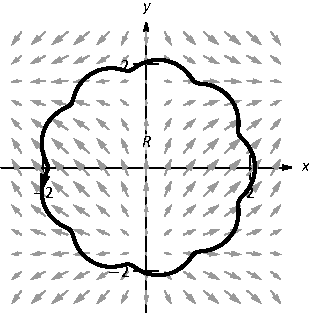
\includegraphics[width=0.4\textwidth]{fig_Vector_Calc_15}
	\caption{The vector field and planar region used in Example \ref{ex_green2}.}
	\label{fig_Vector_Calc_15}
	\end{center}
\end{figure}
\end{example}

One can use Green's theorem to find the area of an enclosed region by integrating along its boundary. Let $C$ be a closed curve, enclosing the region $R$, parametrized by $\vec r(t) = \left( f(t),g(t)\right)$. We know the area of $R$ is computed by the double integral $\iint_R \ dA$, where the integrand is $1$. By creating a field $\vec F$ where $\curl \vec F =1$, we can employ Green's theorem to compute the area of $R$ as $\oint_C \vec F\cdot d\vec r$. 

One is free to choose any field $\vec F$ to use as long as $\curl\vec F = 1$. Common choices are $\vec F = \left( 0,x\right)$, $\vec F = \left( -y,0\right)$ and $\vec F = \left( -y/2,x/2\right)$. We demonstrate this below.


\begin{example}
\label{ex_green3}
Let $C$ be the closed curve parametrized by $\vrt = \left( t-t^3,t^2\right)$ on $-1\leq t\leq 1$, enclosing the region $R$, as shown in Figure \ref{fig_Vector_Calc_16}. Find the area of $R$. 


\begin{figure}[H]
	\begin{center}
			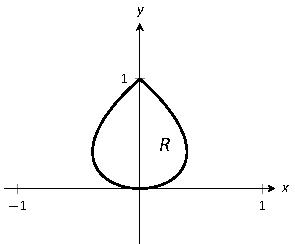
\includegraphics[width=0.4\textwidth]{fig_Vector_Calc_16}
	\caption{The region $R$, whose area is found in Example \ref{ex_green3}}
	\label{fig_Vector_Calc_16}
	\end{center}
\end{figure}


\xhrulefill{gray}{2.5pt}Solution \xhrulefill{gray}{2.5pt}


We can choose any field $\vec F$, as long as $\curl \vec F = 1$. We choose $\vec F = \left( -y,0\right)$. We also confirm (left to the reader) that $\vrt$ traverses the region $R$ in a counterclockwise fashion. Thus the area of $R$ is:
\begin{align*}
A &= \iint_R\ dA \\
									&= \oint_C \vec F\cdot d\vec r\\
									&= \int\limits_{-1}^1 \left( -t^2,0\right)\cdot \left( 1-3t^2,2t\right)\ dt\\
									&= \int\limits_{-1}^1 \left(-t^2 + 3t^4\right)\ dt \\
									&= \frac8{15}.
\end{align*}
\end{example}

\subsection{The divergence theorem}


Green's theorem makes a connection between the circulation around a closed region $R$ and the sum of the curls over $R$. The divergence theorem (also known as Gauss's theorem) makes a somewhat opposite connection: the total flux across the boundary of $R$ is equal to the sum of the divergences over $R$. 



\begin{theorem}[The divergence theorem (in the plane)]
\label{thm:divergence1}
Let $R$ be a closed, bounded region of the plane whose boundary $C$ with unit normal vector $\hat n$ is composed of finitely many smooth curves, let $\vec r(t)$ be a counterclockwise parametrization of $C$ and let $\vec F =\left( M,N\right)$ where $M_x$ and $N_y$ are continuous over $R$. Then
\index{Divergence theorem}\index[aut]{Divergentiestelling}
$$\oint_C \vec F\cdot \hat n\ ds = \iint_R\divv \vec F\ dA.$$
\end{theorem}

A proof of this theorem will be given in Section~\ref{sec:stokes_divergence}, where we will deal with this theorem's counterpart in space.

\begin{example}
\label{ex_div1}
Let $\vec F = \left( x-y,x+y\right)$, let $C$ be the circle of radius 2 centred at the origin and define $R$ to be the interior of that circle, as shown in Figure \ref{fig_Vector_Calc_17}. Verify the divergence theorem; that is, find the flux across $C$ and show it is equal to the double integral of $\divv \vec F$ over $R$.




\xhrulefill{gray}{2.5pt}Solution \xhrulefill{gray}{2.5pt}

We parametrize the circle in the usual way, with $\vrt =\left( 2\cos (t),2\sin (t) \right)$, $0\leq t\leq 2\pi$. The flux across $C$ is
\begin{align*}
\oint_C \vec F\cdot \hat n\ ds &= \oint_C\big(M\,g'(t)-N\, \fp(t)\big)\ dt\\ &= \int\limits_0^{2\pi} \left(\left(2\cos (t)-2\sin (t)\right)\left(2\cos (t)\right) - \left(2\cos (t)+2\sin (t)\right)\left(-2\sin (t)\right)\right)\ dt\\
		&= \int\limits_0^{2\pi} 4\ dt = 8\pi.
\end{align*}
We compute the divergence of $\vec F$ as $\divv \vec F = M_x+N_y = 2$. Since the divergence is constant, we can compute the following double integral easily:
$$\iint_R \divv \vec F\ dA = \iint_R 2\ dA = 2\iint_R\ dA = 2(\text{area of $R$}) = 8\pi,$$
which matches our previous result.

\begin{figure}[H]
	\begin{center}
			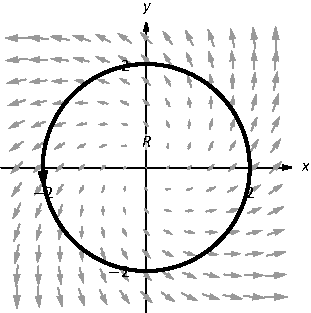
\includegraphics[width=0.4\textwidth]{fig_Vector_Calc_17}
	\caption{The region $R$ used in Example \ref{ex_div1}.}
	\label{fig_Vector_Calc_17}
	\end{center}
\end{figure}
\end{example}


\begin{example}
\label{ex_div2}
Let $\vec F$ be any field where $\divv \vec F = 0$, and let $C_1$ and $C_2$ be any two nonintersecting paths, except that each begins at point $A$ and ends at point $B$ (see Figure \ref{fig_Vector_Calc_18}). Show why the flux across $C_1$ and $C_2$ is the same.

\begin{figure}[H]
	\begin{center}
			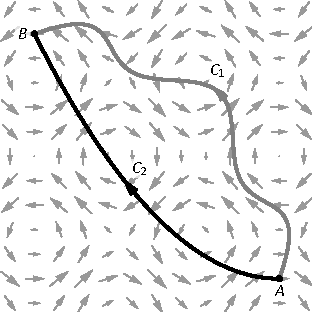
\includegraphics[width=0.37\textwidth]{fig_Vector_Calc_18}
	\caption{As used in Example \ref{ex_div2}, the vector field has a divergence of 0 and the two paths only intersect at their initial and terminal points.}
	\label{fig_Vector_Calc_18}
	\end{center}
\end{figure}


\xhrulefill{gray}{2.5pt}Solution \xhrulefill{gray}{2.5pt}

By referencing Figure \ref{fig_Vector_Calc_18}, we see we can make a closed path $C$ that combines $C_1$ with $C_2$, where $C_2$ is traversed with its opposite orientation. We label the enclosed region $R$. Since $\divv \vec F = 0$, the divergence Theorem states that
$$\oint_C \left(\vec F\cdot \hat n\right)\ ds = \iint_R \divv \vec F\ dA = \iint_R 0\ dA = 0.$$
Recalling the properties of line integrals over vector fields, consider:
\begin{align*}
0 &= \oint_C \left(\vec F\cdot \hat n\right)\ ds \\
 &= \int_{C_1} \left(\vec F\cdot \hat n\right)\ ds +\int_{C_2^*} \left(\vec F\cdot \hat n\right)\ ds\\
	&= \int_{C_1} \left(\vec F\cdot \hat n\right)\ ds -\int_{C_2} \left(\vec F\cdot \hat n\right)\ ds.
\end{align*}
where $C_2^*$ is the path $C_2$ traversed with opposite orientation.
So:
$$\int_{C_1} \left(\vec F\cdot \hat n\right)\ ds = \int_{C_2} \left(\vec F\cdot \hat n\right)\ ds.$$
Thus the flux across each path is equal.
\end{example}

In this section, we have investigated flow and flux, quantities that measure interactions between a vector field and a planar curve. We can also measure flow along spatial curves, though as mentioned before, it does not make sense to measure flux across spatial curves.

It does, however, make sense to measure the amount of a vector field that passes across a surface in space -- i.e, the flux across a surface. We will study this, though in the next section we first  learn about a more powerful way to describe surfaces than using functions of the form $z=f(x,y)$.



\section{Parameterized surfaces and surface area}\label{sec:paramatric_surf_area}
\subsection{Parameterized surfaces}
\label{sec:parametric_surfaces}

	\checkoddpage
\marginpar{\ifoddpage\hspace*{-1.5cm}\else\hspace*{0.25cm}\fi
\includegraphics[width=0.075\textwidth]{youtube}\\
\ifoddpage\hspace*{-1.75cm}\else\hspace*{0.1cm}\fi
\qrcode[height=1.75cm]{https://youtu.be/owKAHXf1y1A}
%\includegraphics[width=0.1\textwidth]{parametrising_surfaces}
}
Thus far we have focused mostly on 2-dimensional vector fields, measuring flow and flux along/across curves in the plane. Both Green's theorem and the divergence theorem make connections between planar regions and their boundaries. We now move our attention to 3-dimensional vector fields, considering both curves and surfaces in space.

We are accustomed to describing surfaces as functions of two variables, usually written as $z=f(x,y)$. For our coming needs, this method of describing surfaces will prove to be insufficient. Instead, we will parametrize our surfaces, describing them as the set of terminal points of some vector--valued function $\vec r(u,v) =\left( f(u,v),g(u,v),h(u,v)\right)$. The bulk of this section is spent practicing the skill of describing a surface \surfaceS\ using a vector--valued function. Once this skill is developed, we'll show how to find the surface area $SA$ of a parametrically--defined surface \surfaceS, a skill needed in the remaining sections of this chapter.

Note that we distinguish a surface from its surface area by using a calligraphic S to denote a surface: \surfaceS. When writing this letter by hand, it may be useful to add serifs to the letter, such as: % 
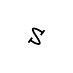
\begin{tikzpicture}[x={(.55ex,0)},y={(0,.55ex)}]
	\draw[smooth, line width=.6pt] (0.9667,0.545) -- (0.8273,0.6541) -- (0.6696,0.7624) -- (0.5,0.866) -- (0.3254,0.961) -- (0.1528,1.043) -- (-0.01133,1.11) -- (-0.1607,1.156) -- (-0.2899,1.181) -- (-0.3945,1.181) -- (-0.471,1.155) -- (-0.5173,1.103) -- (-0.5326,1.025) -- (-0.5173,0.9226) -- (-0.4734,0.7971) -- (-0.4038,0.6515) -- (-0.3127,0.4894) -- (-0.2051,0.3147) -- (-0.08684,0.1318) -- (0.03595,-0.05447) -- (0.1569,-0.2394) -- (0.2696,-0.418) -- (0.3682,-0.5859) -- (0.4473,-0.7388) -- (0.5024,-0.873) -- (0.5299,-0.9855) -- (0.5274,-1.074) -- (0.494,-1.137) -- (0.4299,-1.173) -- (0.3366,-1.184) -- (0.2172,-1.169) -- (0.07558,-1.132) -- (-0.08312,-1.073) -- (-0.253,-0.9971) -- (-0.4276,-0.9068) -- (-0.6001,-0.8063) -- (-0.7635,-0.6994) -- (-0.9113,-0.5902);
	\draw[ line width=.6pt] (-1.18431, -0.959643)--(-0.638322, -0.220787)
								(0.693671, 0.175596)--(1.23965, 0.914452);
\end{tikzpicture}


\begin{definition}[Parametrized surface]
\label{def:parametrized_surface}
Let $\vec r(u,v) = \left(\, f(u,v),g(u,v),h(u,v)\right)$ be a vector--valued function that is continuous and one to one on the interior of its domain $R$ in the $uv$-plane. The set of all terminal points of $\vec r$ (i.e., the range of $\vec r$\,) is the \textbf{surface} (\textit{oppervlak}) \surfaceS, and $\vec r$ along with its domain $R$ form a \textbf{parametrization} (\textit{parametrisering}) of \surfaceS.\\
This parametrization is \textbf{smooth} (\textit{glad}) on $R$ if $\vec r_u$ and $\vec r_v$ are continuous and $\vec r_u\times \vec r_v$ is never $\vec 0$ on the interior of $R$.\index{surface}\index{parametrized surface}\index{smooth!surface}\index{surface!smooth}\index[aut]{oppervlak}
\end{definition}


Given a point $(u_0,v_0)$ in the domain of a vector--valued function $\vec r$, the vectors $\vec r_u(u_0,v_0)$ and $\vec r_v(u_0,v_0)$ are tangent to the surface \surfaceS\ at $\vec r(u_0,v_0)$ (a proof of this is developed later in this section). The definition of smoothness dictates that $\vec r_u\times \vec r_v \neq \vec 0$; this ensures that neither $\vec r_u$ nor $\vec r_v$ are $\vec 0$, nor are they ever parallel. Therefore smoothness guarantees that $\vec r_u$ and $\vec r_v$ determine a plane that is tangent to \surfaceS.

A surface \surfaceS\ is said to be \textbf{orientable} (\textit{ori\"enteerbaar})\index{orientable}\index[aut]{ori\"enteerbaar} if a field of normal vectors can be defined on \surfaceS\ that vary continuously along \surfaceS. This definition may be hard to understand; it may help to know that orientable surfaces are often called two sided. A sphere is an orientable surface, and one can easily envision an inside and outside of the sphere. A paraboloid is orientable, where again one can generally envision  inside and outside sides (or top and bottom sides) to this surface. Just about every surface that one can imagine is orientable, and we'll assume all surfaces we deal with in this text are orientable.

It is enlightening to examine a classic non-orientable surface: the M\"obius band\index{M\"obius band}\index[aut]{M\"obius band}, shown in Figure \ref{fig_Vector_Calc_19}. Vectors normal to the surface are given, starting at the point indicated in the figure. These normal vectors vary continuously as they move along the surface. Letting each vector indicate the top side of the band, we can easily see near any vector which side is the top.
However, if as we progress along the band, we recognize that we are labelling both sides of the band as the top; in fact, there are not two sides to this band, but one. The M\"obius band is a non-orientable surface.


\begin{figure}[H]
	\begin{center}
			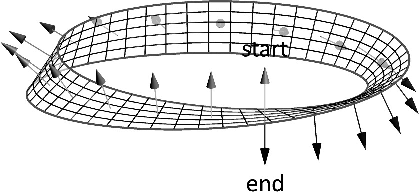
\includegraphics[width=0.4\textwidth]{fig_Vector_Calc_19}
	\caption{A M\"obius band, a non-orientable surface.}
	\label{fig_Vector_Calc_19}
	\end{center}
\end{figure}




We now practice  parameterizing surfaces.



\begin{example}
\label{ex_parsurf1}Parametrize the surface $z=x^2+2y^2$ over the rectangular region $R$ defined by $-3\leq x\leq 3$, $-1\leq y\leq 1$. 




\xhrulefill{gray}{2.5pt}Solution \xhrulefill{gray}{2.5pt}


There is a straightforward way to parametrize a surface of the form $z=f(x,y)$ over a rectangular domain. %Parameterizing surfaces, given in the form $z=f(x,y)$ over rectangular regions is straightforward. 
We  let $x=u$ and $y=v$, and let $\vec r(u,v) = \left( u,v, f(u,v)\right)$. In this instance, we have $\vec r(u,v) = \left( u,v,u^2+2v^2\right)$, for $-3\leq u\leq 3$, $-1\leq v\leq 1$. This surface is graphed in Figure \ref{fig_Vector_Calc_20}.

\begin{figure}[H]
	\begin{center}
			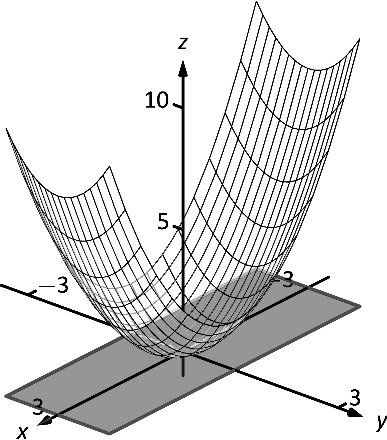
\includegraphics[width=0.4\textwidth]{fig_Vector_Calc_20}
	\caption{The surface parametrized in Example \ref{ex_parsurf1}.}
	\label{fig_Vector_Calc_20}
	\end{center}
\end{figure}

\end{example}

\begin{example}
\label{ex_parsurf2}
Parametrize the surface $z=x^2+2y^2$ over the circular region $R$ enclosed by the circle of radius 2 that is centred at the origin.

\xhrulefill{gray}{2.5pt}Solution \xhrulefill{gray}{2.5pt}


We can parametrize the circular boundary of $R$ with the vector--valued function $\left( 2\cos (u),2\sin (u)\right)$, where $0\leq u\leq 2\pi$. We can obtain the interior of $R$ by scaling this function by a variable amount, i.e., by multiplying by $v$: $\left( 2v\cos (u),2v\sin (u)\right)$, where $0\leq v\leq 1$. 

It is important to understand the role of $v$ in the above function. When $v=1$, we get the boundary of $R$, a circle of radius 2. When $v=0$, we simply get the point $(0,0)$, the center of $R$ (which can be thought of as a circle with radius of 0). When $v=1/2$, we get the circle of radius $1$ that is centred at the origin, which is the circle halfway between the boundary and the center. As $v$ varies from 0 to 1, we create a series of concentric circles that fill out all of $R$.


Thus far, we have determined the $x$- and $y$-components of our parametrization of the surface: $x=2v\cos (u)$ and $y=2v\sin (u)$. We find the $z$-component simply by using $z = f(x,y) = x^2+2y^2$: 
$$z = (2v\cos (u))^2+2(2v\sin (u))^2 = 4v^2\cos^2(u)+8v^2\sin^2(u).$$
Thus $\vec r(u,v) = \left( 2v\cos (u),2v\sin (u),4v^2\cos^2(u)+8v^2\sin^2(u)\right)$, $0\leq u\leq 2\pi$, $0\leq v\leq 1$, which is graphed in Figure \ref{fig_Vector_Calc_21}. The way that this graphic was generated highlights how the surface was parametrized. When viewing from above, one can see lines emanating from the origin; they represent different values of $u$ as $u$ sweeps from an angle of 0 up to $2\pi$. One can also see concentric circles, each corresponding to a different value of $v$. 



\begin{figure}[H]
	\begin{center}
			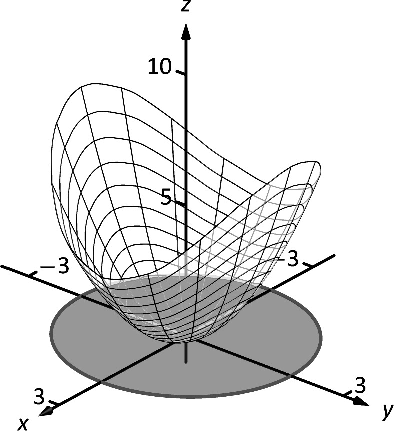
\includegraphics[width=0.4\textwidth]{fig_Vector_Calc_21}
	\caption{The surface parametrized in Example \ref{ex_parsurf2}.}
	\label{fig_Vector_Calc_21}
	\end{center}
\end{figure}


\end{example}


Examples \ref{ex_parsurf1} and \ref{ex_parsurf2} demonstrate an important principle when parameterizing surfaces given in the form $z=f(x,y)$ over a region $R$: if one can determine $x$ and $y$ in terms of $u$ and $v$, then $z$ follows directly as $z=f(x,y)$. 

In the following example, we parametrize the same surface over triangular regions. 


\begin{example}
\label{ex_parsurf4}
Parametrize the surface $z=x^2+2y^2$ over the triangular region $R$ enclosed by the lines \\ $y=3-2x/3$, $y=1$ and $x=0$ as shown in Figure \ref{fig_Vector_Calc_22a}. 

\begin{figure}[H]
\centering
%\raisebox{0.5cm}{
\subfigure[\label{fig_Vector_Calc_22a}]{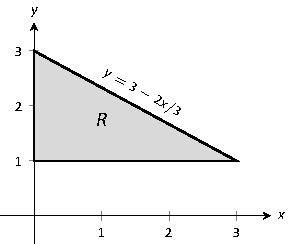
\includegraphics[width=0.43\textwidth]{fig_Vector_Calc_22a}}
\qquad
\subfigure[\label{fig_Vector_Calc_22b}]{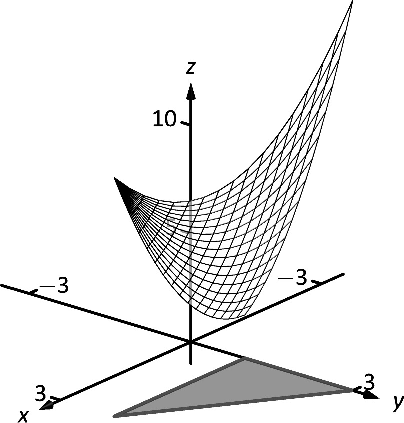
\includegraphics[width=0.43\textwidth]{fig_Vector_Calc_22b} }
\caption{Part (a) shows a graph of the region $R$, and part (b) shows the surface over $R$, as defined in Example \ref{ex_parsurf4}.}
\end{figure}


\pagebreak
\xhrulefill{gray}{2.5pt}Solution \xhrulefill{gray}{2.5pt}

While the region $R$ in this example is very similar to the region $R$ in the previous example, and our method of parameterizing the surface is fundamentally the same, it will feel as though our answer is much different than before.

We begin with letting $x=u$, $0\leq u\leq 3$. We may be tempted to let $y = v(3-2u/3)$, $0\leq v\leq 1$, but this is incorrect. When $v = 1$, we obtain the upper line of the triangle as desired. However, when $v=0$, the $y$-value is 0, which does not lie in the region $R$. 


We will describe the general method of proceeding following this example. For now, consider $y = 1+v(2-2u/3)$, $0\leq v\leq 1$. Note that when $v=1$, we have $y=3-2u/3$, the upper line of the boundary of $R$. Also, when $v=0$, we have $y=1$, which is the lower boundary of $R$. With $z=x^2+2y^2$, we determine $\vec r(u,v) = \left( u, 1+v(2-2u/3), u^2+2\big(1+v(2-2u/3)\big)^2\right)$, $0\leq u\leq 3$, $0\leq v\leq 1$. 

The surface is graphed in Figure \ref{fig_Vector_Calc_22b}.
\end{example}


Given a surface of the form $z=f(x,y)$, one can often determine a parametrization of the surface over a region $R$ in a manner similar to determining bounds of integration over a region $R$. Using the techniques of Section \ref{sec:iterated_integrals}, suppose a region $R$ can be described by $a\leq x\leq b$, $g_1(x) \leq y\leq g_2(x)$, i.e., the area of $R$ can be found using the iterated integral
$$\int\limits_a^b\int\limits_{g_1(x)}^{g_2(x)}\ dy\ dx.$$

When parameterizing the surface, we can let $x=u$, $a\leq u\leq b$, and we can let \\ $y = g_1(u)+v\big(g_2(u)-g_1(u)\big)$, $0\leq v\leq 1$. The parametrization of $x$ is straightforward, but look closely at how $y$ is determined. When $v=0$, $y=g_1(u) = g_1(x)$. When $v=1$, $y= g_2(u)=g_2(x)$. 


 As a specific example, consider the triangular region $R$ from Example \ref{ex_parsurf4}, shown in Figure \ref{fig_Vector_Calc_22a}. Using the techniques of Section \ref{sec:iterated_integrals}, we can find the area of $R$ as
$$\int\limits_0^3\int\limits_1^{3-2x/3} dy\ dx.$$
Following the above discussion, we can set $x=u$, where $0\leq u\leq 3$, and set \\ $y = 1+ v\big(3-2u/3-1\big) = 1+v(2-2u/3)$, $0\leq v\leq 1$, as used in that example.

 So, let a surface \surfaceS\ be the graph of a function $z=f(x,y)$, where the domain of $f$ is  a closed, bounded region $R$ in the $xy$-plane. 
%be the portion of the graph of $z=f(x,y)$ that lies above a region $R$ in the $xy$-plane. 
Let $R$ be bounded by $a\leq x\leq b$, $g_1(x)\leq y\leq g_2(x)$, i.e., the area of $R$ can be found using the iterated integral $\int_a^b\int_{g_1(x)}^{g_2(x)}\ dy\ dx$, and let $h(u,v) = g_1(u)+v\big(g_2(u)-g_1(u)\big)$. 

\surfaceS\ can be parametrized as 
$$\vec r(u,v) = \left( u, h(u,v), f\big(u,h(u,v)\big)\right),\quad a\leq u\leq b,\quad 0\leq v\leq 1.$$

One can do a similar thing if $R$ is bounded by $c\leq y\leq d$, $h_1(y)\leq x\leq h_2(y)$.


\pagebreak
\begin{example}
\label{ex_parsurf5}Find a parametrization of the cylinder $x^2 + z^2/4=1$, where $-1\leq y\leq 2$, as shown in Figure \ref{fig_Vector_Calc_23}. 

\begin{figure}[H]
	\begin{center}
			\includegraphics[width=0.4\textwidth]{fig_Vector_Calc_23}
	\caption{The cylinder parametrized in Example \ref{ex_parsurf5}.}
	\label{fig_Vector_Calc_23}
	\end{center}
\end{figure}

\xhrulefill{gray}{2.5pt}Solution \xhrulefill{gray}{2.5pt}

The equation $x^2+z^2/4=1$ can be envisioned to describe an ellipse in the $xz$-plane; as the equation lacks a $y$-term, the equation describes a cylinder (recall Definition \ref{def:cylinder}) that extends without bound parallel to the $y$-axis. This ellipse has a vertical major axis of length 4, a horizontal minor axis of length 2, and is centred at the origin. We can parametrize this ellipse using sines and cosines; our parametrization can begin with
$$\vec r(u,v) = \left( \cos (u), \text{???}, 2\sin (u)\right),\quad 0\leq u\leq 2\pi,$$
where we still need to determine the $y$-component.

While the cylinder $x^2+z^2/4=1$ is satisfied by any $y$-value, the problem states that all $y$-values are to be between $y=-1$ and $y=2$. Since the value of $y$ does not depend at all on the values of $x$ or $z$, we can use another variable, $v$, to describe $y$. Our final answer is
$$\vec r(u,v) = \left( \cos (u), v, 2\sin (u)\right), \quad 0\leq u\leq 2\pi,\quad -1\leq v\leq 2.$$
\end{example}



\begin{example}
\label{ex_parsurf6}
Find a parametrization of the elliptic cone $$z^2 = \dfrac{x^2}{4}+\dfrac{y^2}{9},$$
where $-2\leq z\leq 3$, as shown in Figure \ref{fig_Vector_Calc_24a}.

\xhrulefill{gray}{2.5pt}Solution \xhrulefill{gray}{2.5pt}

One way to parametrize this cone is to recognize that given a $z$-value, the cross section of the cone at that $z$-value is an ellipse with equation $$\frac{x^2}{(2z)^2} + \frac{y^2}{(3z)^2}=1.$$ We can let $z=v$, for $-2\leq v\leq 3$ and then parametrize the above ellipses using sines, cosines and $v$.  We can parametrize the $x$-component of our surface with $x=2z\cos (u)$ and the $y$-component with $y=3z\sin (u)$, where $0\leq u\leq 2\pi$. Putting all components together, we have
$$\vec r(u,v) = \left( 2v\cos (u), 3v\sin (u), v\right),\quad 0\leq u\leq 2\pi,\quad -2\leq v\leq 3.$$


When $v$ takes on negative values, the radii of the cross--sectional ellipses become negative, which can lead to some surprising results. Consider Figure \ref{fig_Vector_Calc_24b}, where the cone is graphed for $0\leq u\leq \pi$. Because $v$ is negative below the $xy$-plane, the radii of the cross--sectional ellipses are negative, and the opposite side of the cone is sketched below the $xy$-plane.

\begin{figure}[H]
\centering
%\raisebox{0.5cm}{
\subfigure[\label{fig_Vector_Calc_24a}]{\includegraphics[width=0.43\textwidth]{fig_Vector_Calc_24a}}
\qquad
\subfigure[\label{fig_Vector_Calc_24b}]{\includegraphics[width=0.43\textwidth]{fig_Vector_Calc_24b} }
\caption{Part (a) shows the elliptic cone as described in  Example \ref{ex_parsurf6} and part (b) shows the same elliptic cone with restricted domain.}
\end{figure}

\end{example}


Parametrization is a powerful way to represent surfaces. One of the advantages of the methods of parametrization described in this section is that the domain of $\vec r(u,v)$ is always a rectangle; that is, the bounds on $u$ and $v$ are constants. This will make some of our future computations easier to evaluate.

Just as we could parametrize curves in more than one way, there will always be multiple ways to parametrize a surface. Some ways will be more ``natural'' than others, but these other ways are not incorrect. Because technology is often readily available, it is often a good idea to check one's work by graphing a parametrization of a surface to check if it indeed represents what it was intended to.



\subsection{Surface area}
It will become important in the following sections to be able to compute the surface area of a surface \surfaceS\ given a smooth parametrization $\vec r(u,v)$, $a\leq u\leq b$, $c\leq v\leq d$. Following the principles given in the integration review at the beginning of this chapter, we can say that the surface area of \surfaceS\ is given by
$$SA = \iint_{\surfaceS}\ dS,$$
where $dS$ represents a small amount of surface area. That is, to compute total surface area $SA$, add up lots of small amounts of surface area $dS$ across the entire surface \surfaceS. The key to finding surface area is knowing how to compute $dS$. We begin by approximating.

In Section \ref{sec:surface_area} we used the area of a plane to approximate the surface area of a small portion of a surface. We will do the same here.

Let $R$ be the region of the $uv$-plane bounded by $a\leq u\leq b$, $c\leq v\leq d$ as shown in Figure \ref{fig_Vector_Calc_25a}. Partition $R$ into rectangles of width $\Delta u = \frac{b-a}n$ and height $\Delta v = \frac{d-c}n$, for some $n$. Let $p=(u_0,v_0)$ be the lower left corner of some rectangle in the partition, and let $m$ and $q$ be neighbouring corners as shown.

The point with coordinates $\widetilde{P}=(u_0,v_0)$ maps to a point $P = \vec r(u_0,v_0)$ on the surface \surfaceS, and the rectangle with corners $\widetilde{P}$, $\widetilde{M}$ and $\widetilde{Q}$ maps to some region (probably not rectangular) on the surface as shown in Figure \ref{fig_Vector_Calc_25b}, where $M = \vec r(u_0+\Delta\,u,v_0)$ and $Q = \vec r(u_0,v_0+\Delta\,v)$. We wish to approximate the surface area of this mapped region.

Let $\vec u = M-P$ and $\vec v = Q-P$. These two vectors form a parallelogram, illustrated in Figure \ref{fig_Vector_Calc_25c}, whose area approximates the surface area we seek. In this particular illustration, we can see that parallelogram does not particularly match well the region we wish to approximate, but that is acceptable; by increasing the number of partitions of $R$, $\Delta u$ and $\Delta v$ shrink and our approximations will become better.


\begin{figure}[H]
\centering
%\raisebox{0.5cm}{
\subfigure[\label{fig_Vector_Calc_25a}]{\includegraphics[width=0.35\textwidth]{fig_Vector_Calc_25a}}
\qquad
\subfigure[\label{fig_Vector_Calc_25b}]{\includegraphics[width=0.3\textwidth]{fig_Vector_Calc_25b} }
\qquad
\subfigure[\label{fig_Vector_Calc_25c}]{\includegraphics[width=0.3\textwidth]{fig_Vector_Calc_25c} }
\caption{Illustrating the process of finding surface area by approximating with planes.}
\end{figure}


From Section \ref{sec:cross_product} we know the area of this parallelogram is $\norm{\vec u\times \vec v}$. If we repeat this approximation process for each rectangle in the partition of $R$, we can sum the areas of all the parallelograms to get an approximation of the surface area $SA$:
$$SA \approx \sum_{j=1}^n\sum_{i=1}^n \ \norm{\vec u_{i,j}\times \vec v_{i,j}},$$
where $\vec u_{i,j} = \vec r(u_i+\Delta u,v_j) - \vec r(u_i,v_j)$ and $\vec v_{i,j} = \vec r(u_i,v_j+\Delta v)-\vec r(u_i,v_j)$.

From our previous calculus experience, we expect that taking a limit as $n\to +\infty$ will result in the exact surface area. However, the current form of the above double sum makes it difficult to realize what the result of that limit is. The following rewriting of the double summation will be helpful:

\begin{align*}
\sum_{j=1}^n\sum_{i=1}^n \ \norm{\vec u_{i,j}\times \vec v_{i,j}}&= \sum_{j=1}^n\sum_{i=1}^n \ \norm{\big(\vec r(u_i+\Delta u,v_j) - \vec r(u_i,v_j)\big) \times \big(\vec r(u_i,v_j+\Delta v)-\vec r(u_i,v_j)\big)} \\
&= \sum_{j=1}^n\sum_{i=1}^n \ \norm{\frac{\vec r(u_i+\Delta u,v_j) - \vec r(u_i,v_j)}{\Delta u} \times \frac{\vec r(u_i,v_j+\Delta v)-\vec r(u_i,v_j)}{\Delta v}}\Delta u\Delta v.
\end{align*}

We now take the limit as $n\to+\infty$, forcing $\Delta u$ and $\Delta v$ to 0. As $\Delta u\to 0$,
$$\frac{\vec r(u_i+\Delta u,v_j) - \vec r(u_i,v_j)}{\Delta u}\quad \to\quad \vec r_u(u_i,v_j)\,, $$
and as $\Delta v\to 0$,
$$\frac{\vec r(u_i,v_j+\Delta v)-\vec r(u_i,v_j)}{\Delta v}\quad \to\quad \vec r_v(u_i,v_j).$$
This limit process also demonstrates that $\vec r_u(u,v)$ and $\vec r_v(u,v)$ are tangent to the surface \surfaceS\ at $\vec r(u,v)$. We do not need this fact now, but it will be important in the next section.

Thus, in the limit, the double sum leads to a double integral:
$$\lim_{n\to+\infty} \sum_{j=1}^n\sum_{i=1}^n \ \norm{\vec u_{i,j}\times \vec v_{i,j}}= \int\limits_c^d\int\limits_a^b \norm{\vec r_u\times\vec r_v}\ du\ dv.$$

\begin{theorem}[Surface area of parametrically defined surfaces]
\label{thm:par_surface_area}
Let $\vec r(u,v)$ be a smooth parametrization of a surface \surfaceS\ over a closed, bounded region $R$ of the $uv$-plane.
\begin{itemize}
\item	The surface area differential $dS$ is: $dS = \norm{\vec r_u\times \vec r_v}\ dA$.
\item The surface area $SA$ of \surfaceS\ is
$$SA = \iint_\surfaceS\ dS = \iint_R \norm{\vec r_u\times \vec r_v}\ dA.$$
\end{itemize}
\end{theorem}


\begin{example}
\label{ex_parsurfarea1}Using the parametrization found in Example \ref{ex_parsurf2}, find the surface area of $z=x^2+2y^2$ over the circular disk of radius 2, centred at the origin.

\xhrulefill{gray}{2.5pt}Solution \xhrulefill{gray}{2.5pt}

In Example \ref{ex_parsurf2}, we parametrized the surface as \\ $\vec r(u,v) = \left( 2v\cos (u), 2v\sin (u), 4v^2\cos^2(u)+8v^2\sin^2(u)\right)$, for $0\leq u\leq 2\pi$, $0\leq v\leq 1$. To find the surface area using Theorem \ref{thm:par_surface_area}, we need $\norm{\vec r_u\times\vec r_v}$. We find:
\begin{align*}
\vec r_u &= \left( -2v\sin (u), 2v\cos (u), 8v^2\cos (u)\sin (u)\right)\\
\vec r_v &= \left( 2\cos (u), 2\sin (u), 8v\cos^2 (u)+16v\sin^2(u)\right)\\
&= \left( 2\cos (u), 2\sin (u), 16v -8v\cos^2 (u)\right)\\
\Rightarrow \ \vec r_u\times\vec r_v &= \left( 16v^2\cos (u), 32v^2\sin (u), -4v\right)\\
\Rightarrow \ \norm{\vec r_u\times\vec r_v} &= \sqrt{256v^4\cos^2(u)+1024v^4\sin^2(u)+16v^2}\, .
\end{align*}
Thus the surface area $SA$ is
\begin{align*}
\iint_\surfaceS \ dS &= \iint_R\norm{\vec r_u\times \vec r_v}\ dA \\
& = \int\limits_0^1\int\limits_0^{2\pi} \sqrt{256v^4\cos^2(u)+1024v^4\sin^2(u)+16v^2}\ du\ dv \approx 53.59.
\end{align*}
There is a lot of tedious work in the above calculations and the final integral is nontrivial. The use of a computer-algebra system is highly recommended.
\end{example}

In Section \ref{sec:line_int_intro}, we recalled the arc length differential $ds=\norm{\vrp(t)}dt$. In subsequent sections, we used that differential, but in most applications the $\norm{\vrp(t)}$ in the differential canceled out of the integrand (to our benefit, as integrating the square roots of functions is generally difficult). We will find a similar thing happens when we use the surface area differential $dS$ in the following sections. That is, our main goal is not to be able to compute surface area; rather, surface area is a tool to obtain other quantities that are more important and useful. In our applications, we will use $dS$, but most of the time the $\norm{\vec r_u\times \vec r_v}$ part will cancel out of the integrand, making the subsequent integration easier to compute.


\section{Surface integrals}\label{sec:surf_int}
\subsection{Definition}

Consider a smooth surface \surfaceS\ that represents a thin sheet of metal. How could we find the mass of this metallic object?

If the density of this object is constant, then we can find mass via mass$=$ density $\times$ surface area, and we could compute the surface area using the techniques of the previous section. 

What if the density were not constant, but variable, described by a function $\delta(x,y,z)$? We can describe the mass using our general integration techniques as
$$\text{mass} = \iint_\surfaceS \ dm,$$
where $dm$ represents a little bit of mass. That is, to find the total mass of the object, sum up lots of little masses over the surface.

How do we find the little bit of mass $dm$? On a small portion of the surface with surface area $\Delta S$, the density is approximately constant, hence $dm \approx \delta(x,y,z)\Delta S$. As we use limits to shrink the size of $\Delta S$ to 0, we get $dm = \delta(x,y,z)dS$; that is, a little bit of mass is equal to a density times a small amount of surface area. Thus the total mass of the thin sheet is
\begin{equation}
\text{mass} =\iint_\surfaceS \delta(x,y,z)\ dS.\label{eq:surface_int}
\end{equation}

To evaluate the above integral, we would seek $\vec r(u,v)$, a smooth parametrization of \surfaceS\ over a region $R$ of the $uv$-plane. The density would become a function of $u$ and $v$, and we would integrate $\iint_R \delta(u,v)\ \norm{\vec r_u\times \vec r_v}\ dA.$

The integral in Equation \eqref{eq:surface_int} is a specific example of a more general construction defined below.


\begin{definition}[Surface integral]
\label{def:surface_integral}
Let $G(x,y,z)$ be a continuous function defined on a surface \surfaceS. The \textbf{surface integral} \textit{(oppervlakte-integraal)} of $G$ on \surfaceS\ is\index{surface integral}
$$\iint_\surfaceS G(x,y,z)\ dS.$$
\end{definition}

Surface integrals can be used to measure a variety of quantities beyond mass. If $G(x,y,z)$ measures the static charge density at a point, then the surface integral will compute the total static charge of the sheet. If $G$ measures the amount of fluid passing through a screen (represented by \surfaceS) at a point, then the surface integral gives the total amount of fluid going through the screen.


\begin{example}
\label{ex_surfint1}
Find the mass of a thin sheet modeled by the plane $2x+y+z=3$ over the triangular region of the $xy$-plane bounded by the coordinate axes and the line $y=2-2x$, as shown in Figure \ref{fig_Vector_Calc_26}, with density function $\delta(x,y,z) = x^2+5y+z$, where all distances are measured in cm and the density is given as g/cm$^2$. 

\begin{figure}[H]
	\begin{center}
			\includegraphics[width=0.4\textwidth]{fig_Vector_Calc_26}
	\caption{The surface whose mass is computed in Example \ref{ex_surfint1}.}
	\label{fig_Vector_Calc_26}
	\end{center}
\end{figure}

\xhrulefill{gray}{2.5pt}Solution \xhrulefill{gray}{2.5pt}


We begin by parameterizing the planar surface \surfaceS. Using the techniques of the previous section, we can let $x=u$ and $y=v(2-2u)$, where $0\leq u\leq 1$ and $0\leq v\leq 1$. Solving for $z$ in the equation of the plane, we have $z=3-2x-y$, hence $z = 3-2u-v(2-2u)$, giving the parametrization
$\vec r(u,v) = \left( u, v(2-2u), 3-2u-v(2-2u)\right)$.


We need $dS=\norm{\vec r_u \times \vec r_v}\ dA$, so we need to compute $\vec r_u$, $\vec r_v$ and the norm of their cross product. We leave it to the reader to confirm the following:
$$\vec r_u = \left( 1,-2v,2v-2\right),\quad \vec r_v = \left( 0,2-2u, 2u-2\right),$$
$$\vec r_u\times \vec r_v = \left( 4-4u,2-2u,2-2u\right)\quad \text{and }\quad \norm{\vec r_u\times \vec r_v} = 2\sqrt{6}\sqrt{(u-1)^2}.$$
We need to be careful to not simplify \ $\norm{\vec r_u\times \vec r_v} = 2\sqrt{6}\sqrt{(u-1)^2}$ \  as \  $2\sqrt{6}(u-1)$; rather, it is \\ $2\sqrt{6}|u-1|$. In this example, $u$ is bounded by $0\leq u\leq 1$, and on this interval $|u-1| = 1-u$. Thus $dS = 2\sqrt{6}(1-u)\ dA$. 

The density is given as a function of $x$, $y$ and $z$, for which we will substitute the corresponding components of $\vec r$: 
\begin{align*}
\delta(x,y,z) &= \delta\big(\vec r(u,v) \big) \\
			&= u^2 + 5v(2-2u)+3-2u-v(2-2u)\\
			&= u^2-8uv-2u+8v+3.
\end{align*}
Thus the mass of the sheet is:
\begin{align*}
M &= \iint_\surfaceS\ dm\\
	&= \iint_R \delta\big(\vec r(u,v)\big)\ \norm{\vec r_u\times \vec r_v}\ dA\\
	&= \int\limits_0^1\int\limits_0^1 \left(u^2-8uv-2u+8v+3\big)\big(2\sqrt{6}(1-u)\right)\ du\ dv\\
	&= \frac{31}{\sqrt{6}} \approx 12.66 \text{ g.}
\end{align*}

\end{example}

\subsection{Flux}

	\checkoddpage
\marginpar{\ifoddpage\hspace*{-1.5cm}\else\hspace*{0.25cm}\fi\includegraphics[width=0.075\textwidth]{youtube}\\
\ifoddpage\hspace*{-1.75cm}\else\hspace*{0.1cm}\fi
\qrcode[height=1.75cm]{https://youtu.be/ivg3dLTarbs}
%\includegraphics[width=0.1\textwidth]{flux_3d}
}
Let a surface \surfaceS\ lie within a vector field $\vec F$. One is often interested in measuring the flux of $\vec F$ across \surfaceS; that is, measuring how much of the vector field passes across \surfaceS. For instance, if $\vec F$ represents the velocity field of moving air and \surfaceS\ represents the shape of an air filter, the flux will measure how much air is passing through the filter per unit time.\index{flux}\index[aut]{flux}

As flux measures the amount of $\vec F$ passing across \surfaceS, we need to find the amount of $\vec F$ orthogonal to \surfaceS. Similar to our measure of flux in the plane, this is equal to $\vec F\cdot \hat n$, where $\hat n$ is a unit vector normal to \surfaceS\ at a point. We now consider how to find $\hat n$.

Given a smooth parametrization $\vec r(u,v)$ of \surfaceS, the work in the previous section showing the development of our method of computing surface area also shows that $\vec r_u(u,v)$ and $\vec r_v(u,v)$ are tangent to \surfaceS\ at $\vec r(u,v)$. Thus $\vec r_u\times \vec r_v$ is orthogonal to \surfaceS, and we let
$$\hat n = \frac{\vec r_u\times \vec r_v}{\norm{\vec r_u\times \vec r_v}},$$
which is a unit vector normal to \surfaceS\ at $\vec r(u,v)$.

The measurement of flux across a surface is a surface integral; that is, to measure total flux we sum the product of $\vec F\cdot\hat n$ times a small amount of surface area: $\vec F\cdot \hat n\ dS$. 

A nice thing happens with the actual computation of flux: the $\norm{\vec r_u\times \vec r_v}$ terms go away. Consider:
\begin{align*}
\text{flux} &= \iint_\surfaceS \vec F\cdot \hat n\ dS \\
				&= \iint_R \vec F\cdot \frac{\vec r_u\times \vec r_v}{\norm{\vec r_u\times \vec r_v}}\ \norm{\vec r_u\times \vec r_v}\ dA \\
				&= \iint_R \vec F\cdot (\vec r_u\times \vec r_v)\ dA.
\end{align*}

Recall that $R$ is the region in the $uv$-plane that we get by projecting \surfaceS\ onto that plane.  The above only makes sense if \surfaceS\ is orientable; the normal vectors $\hat n$ must vary continuously across \surfaceS. We assume that $\hat n$ does vary continuously. If the parametrization $\vec r$ of \surfaceS\ is smooth, then our above definition of $\hat n$ will vary continuously.

\begin{definition}[Flux across a surface]
\label{def:surfflux}
Let $\vec F$ be a vector field with continuous components defined on an orientable surface \surfaceS\ with normal vector $\hat n$. The \textbf{flux of $\vec F$ across \surfaceS\ }is\index{flux}
$$\text{flux} = \iint_\surfaceS \vec F\cdot \hat n\ dS.$$
If \surfaceS\ is parametrized by $\vec r(u,v)$, which is smooth on its domain $R$, then
$$\text{flux} = \iint_R \vec F\big(\vec r(u,v)\big)\cdot (\vec r_u\times \vec r_v)\ dA.$$
\end{definition}

Since \surfaceS\ is orientable, we adopt the convention of saying one passes from the back side of \surfaceS\ to the front side when moving across the surface parallel to the direction of $\hat n$. Also, when \surfaceS\ is closed, it is natural to speak of the regions of space inside and outside \surfaceS. We also adopt the convention that when \surfaceS\ is a closed surface, $\hat n$ should point to the outside of \surfaceS. If $\hat n = \vec r_u\times\vec r_v$ points inside \surfaceS, use $\hat n = \vec r_v\times \vec r_u$ instead.

When the computation of flux is positive, it means that the field is moving from the back side of \surfaceS\ to the front side; when flux is negative, it means the field is moving opposite the direction of $\hat n$, and is moving from the front of \surfaceS\ to the back. When \surfaceS\ is not closed, there is not a right and wrong direction in which $\hat n$ should point, but one should be mindful of its direction to make full sense of the flux computation.

We demonstrate the computation of flux, and its interpretation, in the following examples.


\begin{example}
\label{ex_surfflux1}
Let \surfaceS\ be the surface given in Example \ref{ex_surfint1}, where \surfaceS\ is parametrized by \\ $\vec r(u,v) = \left( u, v(2-2u),3-2u-v(2-2u)\right)$ on $0\leq u\leq 1$, $0\leq v\leq 1$, and let $\vec F = \left( 1, x,-y\right)$, as shown in Figure \ref{fig_Vector_Calc_27}. Find the flux of $\vec F$ across \surfaceS.


\begin{figure}[H]
	\begin{center}
			\includegraphics[width=0.4\textwidth]{fig_Vector_Calc_27}
	\caption{The surface and vector field used in  Example \ref{ex_surfflux1}.}
	\label{fig_Vector_Calc_27}
	\end{center}
\end{figure}

\xhrulefill{gray}{2.5pt}Solution \xhrulefill{gray}{2.5pt}

Using our work from the previous example, we have $\hat n = \vec r_u\times\vec r_v = \left( 4-4u,2-2u,2-2u\right)$. We also need $\vec F\big(\vec r(u,v)\big) = \left( 1, u, -v(2-2u)\right)$. 

Thus the flux of $\vec F$ across \surfaceS\ is:
\begin{align*}
\text{flux} &= \iint_\surfaceS \vec F\cdot \hat n\ dS\\
			&= \iint_R \left( 1,u,-v(2-2u)\right)\cdot\left( 4-4u,2-2u,2-2u\right)\ dA \\
			&= \int\limits_0^1\int\limits_0^1 \big(-4u^2v-2u^2+8uv-2u-4v+4\big)\ du\ dv\\
			&= \dfrac{5}{3}.
\end{align*}
To make full use of this numeric answer, we need to know the direction in which the field is passing across \surfaceS. The graph in Figure \ref{fig_Vector_Calc_27} helps, but we need a method that is not dependent on a graph.

Pick a point $(u,v)$ in the interior of $R$, which is the region in the $uv$-plane that we get by projecting \surfaceS\ onto that plane, and consider $\hat n(u,v)$. For instance, choose $(u,v)=(1/2,1/2)$ and look at $\hat n\left(\vec r(1/2,1/2)\right) = \left( 2,1,1\right)/\sqrt{6}$. This vector has positive $x$-, $y$- and $z$-components. Generally speaking, one has some idea of what the surface \surfaceS\ looks like, as that surface is for some reason important. In our case, we know \surfaceS\ is a plane with $z$-intercept of $z=3$. Knowing $\hat n$ and the flux measurement of positive $5/3$, we know that the field must be passing from behind \surfaceS, i.e., the side the origin is on, to the front of \surfaceS.
\end{example}

\begin{example}
\label{ex_surfflux2}
Let $\surfaceS_1$ be the unit disk in the $xy$-plane, and let $\surfaceS_2$ be the paraboloid $z=1-x^2-y^2$, for $z\geq 0$, as graphed in Figure \ref{fig_Vector_Calc_28}. Note how these two surfaces each have the unit circle as a boundary.
 

Let $\vec F_1 = \left( 0,0,1\right)$ and $\vec F_2 = \left( 0,0,z\right)$. Using normal vectors for each surface that point upward, i.e., with a positive $z$-component, find the flux of each field across each surface. 

\begin{figure}[H]
	\begin{center}
			\includegraphics[width=0.4\textwidth]{fig_Vector_Calc_28}
	\caption{The surfaces used in  Example \ref{ex_surfflux2}.}
	\label{fig_Vector_Calc_28}
	\end{center}
\end{figure}


\xhrulefill{gray}{2.5pt}Solution \xhrulefill{gray}{2.5pt}

We begin by parameterizing each surface.

The boundary of the unit disk in the $xy$-plane is the unit circle, which can be described with $\left( \cos (u),\sin (u),0\right)$, $0\leq u\leq 2\pi$. To obtain the interior of the circle as well, we can scale by $v$, giving
$$\vec r_1(u,v) = \left( v\cos (u),v\sin (u), 0\right), \quad 0\leq u\leq 2\pi, \quad 0\leq v\leq 1.$$

As the boundary of $\surfaceS_2$ is also the unit circle, the $x$- and $y$-components of $\vec r_2$ will be the same as those of $\vec r_1$; we just need a different $z$ component. With $z = 1-x^2-y^2$, we have
$$\vec r_2(u,v) = \left( v\cos (u),v\sin (u), 1-v^2\cos^2(u)-v^2\sin^2(u)\right) = \left( v\cos (u),v\sin (u), 1-v^2\right),$$
where $0\leq u\leq 2\pi$ \ and \ $0\leq v\leq 1$.

We now compute the normal vectors $\hat n_1$ and $\hat n_2$.

For $\hat n_1$: $\left(\vec r_{1}\right)_u= \left( -v\sin (u), v\cos (u),0\right)$,\  $ \left(\vec r_{1}\right)_v = \left( \cos (u),\sin (u),0\right)$, so
$$\hat n_1 = \left(\vec r_{1}\right)_u\times  \left(\vec r_{1}\right)_v = \left( 0,0,-v\right).$$
As this vector has a negative $z$-component, we instead use
$$\hat n_1 = \left(\vec r_{1}\right)_v\times \left(\vec r_{1}\right)_u = \left( 0,0,v\right).$$

Similarly, $\hat n_2$: $\left(\vec r_{2}\right)_u= \left( -v\sin (u), v\cos (u),0\right)$, \ $\left(\vec r_{2}\right)_v = \left( \cos (u),\sin (u),-2v\right)$, so 
$$\hat n_2 = \left(\vec r_{2}\right)_u\times \left(\vec r_{2}\right)_v = \left( -2v^2\cos (u),-2v^2\sin (u),-v\right).$$ 
Again, this normal vector has a negative $z$-component so we use
$$\hat n_2 = \left(\vec r_{2}\right)_v\times \left(\vec r_{2}\right)_u = \left( 2v^2\cos (u),2v^2\sin (u),v\right).$$ 

We are now set to compute flux. Over field $\vec F_1=\left( 0,0,1\right)$:
\begin{align*}
\text{flux across $\surfaceS_1$} &= \iint_{\surfaceS_1} \vec F_1\cdot \hat n_1\ dS \\
						&= \iint_R\left( 0,0,1\right)\cdot\left( 0,0,v\right)\ dA\\
						&= \int\limits_0^1\int\limits_0^{2\pi} (v)\ du\ dv\\
						&= \pi.
\end{align*}
\begin{align*}
\text{flux across $\surfaceS_2$} &= \iint_{\surfaceS_2} \vec F_1\cdot \hat n_2\ dS \\
						&= \iint_R\left( 0,0,1\right)\cdot\left( 2v^2\cos (u),2v^2\sin (u),v\right)\ dA\\
						&= \int\limits_0^1\int\limits_0^{2\pi} (v)\ du\ dv\\
						&= \pi.
\end{align*}

These two results are equal and positive. Each are positive because both normal vectors are pointing in the positive $z$-directions, as does $\vec F_1$. As the field passes through each surface in the direction of their normal vectors, the flux is measured as positive.

We can also intuitively understand why the results are equal. Consider $\vec F_1$ to represent the flow of air, and let each surface represent a filter. Since $\vec F_1$ is constant, and moving straight up, it makes sense that all air passing through $\surfaceS_1$ also passes through $\surfaceS_2$, and vice--versa. 

If we treated the surfaces as creating one piecewise smooth surface \surfaceS, we would find the total flux across \surfaceS\ by finding the flux across each piece, being sure that each normal vector pointed to the outside of the closed surface. Above, $\hat n_1$ does not point outside the surface, though $\hat n_2$ does. We would instead want to use $-\hat n_1$ in our computation. We would then find that the flux across $\surfaceS_1$ is $-\pi$, and hence the total flux across \surfaceS\ is $-\pi + \pi = 0$. As $0$ is a special number, we should wonder if this answer has special significance. It does, which is briefly discussed following this example and will be more fully developed in the next section.

We now compute the flux across each surface with $\vec F_2=\left( 0,0,z\right)$. First, the flux across $\surfaceS_1$: 
\begin{align*}
&\iint_{\surfaceS_1} \vec F_2\cdot \hat n_1\ dS .
\intertext{Over $\surfaceS_1$, $\vec F_2 = \vec F_2\big(\vec r_1(u,v)\big) = \left( 0,0,0\right).$ Therefore,}
\text{flux across $\surfaceS_1$} &= \iint_R\left( 0,0,0\right)\cdot\left( 0,0,v\right)\ dA\\
						&= \int\limits_0^1\int\limits_0^{2\pi} (0)\ du\ dv\\
						&= 0.
\end{align*}
Then, the flux across $\surfaceS_2$: 
\begin{align*}
 &\iint_{\surfaceS_2} \vec F_2\cdot \hat n_2\ dS .
\intertext{Over $\surfaceS_2$, $\vec F_2 = \vec F_2\big(\vec r_2(u,v)\big) = \left( 0,0,1-v^2\right).$ Therefore,}
\text{flux across $\surfaceS_2$} &= \iint_R\left( 0,0,1-v^2\right)\cdot\left( 2v^2\cos (u),2v^2\sin (u),v\right)\ dA\\
						&= \int\limits_0^1\int\limits_0^{2\pi} (v-v^3)\ du\ dv\\
						&= \dfrac{\pi}{2}.
\end{align*}

This time the measurements of flux differ. Over $\surfaceS_1$, the field $\vec F_2$ is just $\vec 0$, hence there is no flux. Over $\surfaceS_2$, the flux is again positive as $\vec F_2$ points in the positive $z$-direction over $\surfaceS_2$, as does $\hat n_2$.
\end{example}

In the previous example, the surfaces $\surfaceS_1$ and $\surfaceS_2$ form a closed surface that is piecewise smooth. That the measurement of flux across each surface was the same for some fields (and not for others) is reminiscent of a result from Section \ref{sec:greensthm}, where we measured flux across curves. The quick answer to why the flux was the same when considering $\vec F_1$ is that $\divv \vec F_1 = 0$. In the next section, we'll see the second part of the Divergence Theorem which will more fully explain this occurrence. We will also explore Stokes' theorem, the spatial analogue to Green's theorem.



\section{The divergence theorem revisited and Stokes' theorem}\label{div_stelling_3D_stokes}
\subsection{The divergence theorem}

\label{sec:stokes_divergence}


	\checkoddpage
\marginpar{\ifoddpage\hspace*{-1.5cm}\else\hspace*{0.25cm}\fi\includegraphics[width=0.075\textwidth]{youtube}\\
\ifoddpage\hspace*{-1.75cm}\else\hspace*{0.1cm}\fi
\qrcode[height=1.75cm]{https://youtu.be/UOG3mOhv5Xo}
%\includegraphics[width=0.1\textwidth]{divergence_theorem}
}
Theorem \ref{thm:divergence1} gives the divergence theorem in the plane, which states that the flux of a vector field across a closed \textit{curve} equals the sum of the divergences over the region enclosed by the curve. Recall that the flux was measured via a line integral, and the sum of the divergences was measured through a double integral.

We now consider the three-dimensional version of the divergence theorem. It states, in words, that the flux across a closed \textit{surface} equals the sum of the divergences over the domain enclosed by the surface. Since we are in space (versus the plane), we measure flux via a surface integral, and the sums of divergences will be measured through a triple integral.

\begin{theorem}[The divergence theorem (in space)]
\label{thm:divergence2}
Let $D$ be a closed domain in space whose boundary is an orientable, piecewise smooth surface \surfaceS\ with outer unit normal vector $\hat n$, and let $\vec F$ be a vector field whose components are differentiable on $D$. Then\index{Divergence Theorem!in space}
$$\iiint_D \divv \vec F\ dV=\iint_\surfaceS \vec F\cdot\hat n\ dS .$$ 
\end{theorem}

Note that the term outer unit normal vector used in Theorem \ref{thm:divergence2} means $\hat n$ points to the outside of \surfaceS.\index{outer unit normal vector}

\begin{proof}
It suffices to prove the theorem for rectangular prisms; the Riemann sum nature of the triple integral then guarantees the theorem for arbitrary regions. So, let 
$$
    D=\left\{(x,y,z)\left|a_1\leq x\leq a_2,b_1\leq y\leq b_2,c_1\leq z\leq c_2 \right.\right\}
$$
and let $S$ be the boundary surface of $R$. Then
$$
    S=A_1\cup A_2\cup A_3\cup A_4\cup A_5\cup A_6
$$
where $A_1$ and $A_2$ are those sides perpendicular to the $x$-axis, $A_3$ and $A_4$ are those sides perpendicular to the $y$-axis and $A_5$ and $A_6$ are those sides perpendicular to the $z$-axis. Furthermore, we let \\ $\vec F = M\, \hat{\imath} + N\, \hat{\jmath} + P\, \hat{k}$, where $M,\,N,\,P:\mathbb{R}^3\mapsto\mathbb{R}$. 

Then, we have
\begin{eqnarray*}
\displaystyle \iiint_D \vec{\nabla} \cdot \vec F \ dV&=&\displaystyle \iiint_D \left({ \frac{\partial M}{\partial x} + \frac{\partial N}{\partial y} + \frac{\partial P}{\partial z} }\right) \ dx \ dy \ dz\\[0.2cm]
&=&\displaystyle \iiint_D \frac{\partial M}{\partial x} \ dx \ dy \ dz + \iiint_D \frac{\partial N}{\partial y} \ dx \ dy \ dz + \iiint_D \frac{\partial P}{\partial z} \ dx \ dy \ dz\\[0.2cm]
&=&\displaystyle \int\limits_{c_1}^{c_2} \int\limits_{b_1}^{b_2} \left({M \left({a_2, y, z}\right) - M \left({a_1, y, z}\right)}\right) \ dy \ dz +\displaystyle \int\limits_{c_1}^{c_2} \int\limits_{a_1}^{a_2} \left({N \left({x, b_2, z}\right) - N \left({x, b_1, z}\right)}\right) \ dx \ dz\\[0.2cm]
&+&\displaystyle \int\limits_{b_1}^{b_2} \int\limits_{a_1}^{a_2} \left({P \left({x, y, c_2}\right) - P \left({x, y, c_1}\right)}\right) \ dx \ dy\\[0.2cm]
&=&\displaystyle \iint_{A_2} M \ dy \ dz - \iint_{A_1} M \ dy \ dz+\displaystyle \iint_{A_4} N \ dx \ dz - \iint_{A_3} N \ dx \ dz\\[0.2cm]
&+&\displaystyle \iint_{A_6} P \ dx \ dy - \iint_{A_5} P \ dx \ dy
\end{eqnarray*}
We turn now to examine $\hat{n}$:
\begin{eqnarray*}
\hat{n}&=&\displaystyle \left({-1, 0, 0}\right)\quad\text{on}\quad\,A_1,\\
\hat{n}&=&\displaystyle \left({1, 0, 0}\right)\quad\text{on}\quad\,A_2,\\
\hat{n}&=&\displaystyle \left({0, -1, 0}\right)\quad\text{on}\quad\,A_3,\\
\hat{n}&=&\displaystyle \left({0, 1, 0}\right)\quad\text{on}\quad\,A_4,\\
\hat{n}&=&\displaystyle \left({0, 0, -1}\right)\quad\text{on}\quad\,A_5,\\
\hat{n}&=&\displaystyle \left({0, 0, 1}\right)\quad\text{on}\quad\,A_6.\\
\end{eqnarray*} 
Hence, we have
\begin{eqnarray*}
\vec{F}\cdot\hat{n}&=&-M\quad\text{on}\quad\,A_1,\\
\vec{F}\cdot\hat{n}&=&M\quad\text{on}\quad\,A_2,\\
\vec{F}\cdot\hat{n}&=&-N\quad\text{on}\quad\,A_3,\\
\vec{F}\cdot\hat{n}&=&N\quad\text{on}\quad\,A_4,\\
\vec{F}\cdot\hat{n}&=&-P\quad\text{on}\quad\,A_5,\\
\vec{F}\cdot\hat{n}&=&P\quad\text{on}\quad\,A_6.\\
\end{eqnarray*} 
Besides, we also have that
\begin{eqnarray*}
dS&=&dy\ dz\quad\text{on}\quad\,A_1\ \text{ and }\ A_2,\\
dS&=&dx\ dz\quad\text{on}\quad\,A_3\ \text{ and }\ A_4,\\
dS&=&dx\ dy\quad\text{on}\quad\,A_5\ \text{ and }\ A_6,\\
\end{eqnarray*} 
where $dS$ is the area element. This is true because each side is perfectly flat, and constant with respect to one coordinate. 
Consequently
$$
\displaystyle \iint_{A_2} \vec F\cdot\hat n \ dS=\displaystyle \iint_{A_2} M \ dy \ dz
$$
and in general
\begin{multline*}
\displaystyle \sum_{i = 1}^6 \iint_{A_i} \vec F\cdot\hat n \ dS=\displaystyle \iint_{A_2} M \ dy \  dz - \iint_{A_1} M \ dy \ dz + \iint_{A_4} N \ dx \ dz - \iint_{A_3} N \ dx \ dz\ +\\[0.2cm]
 \iint_{A_6} P \ dx \ dy - \iint_{A_5} P \ dx \ dy\,.
\end{multline*}
Hence, the result
$$\iiint_D \divv \vec F\ dV=\iint_\surfaceS \vec F\cdot\hat n\ dS .$$

\end{proof}

\begin{example}
\label{ex_divthm_space2}
Let $D$ be the domain in space bounded by the planes $z=0$ and $z=2x$, along with the cylinder $x=1-y^2$, as graphed in Figure \ref{fig_Vector_Calc_29}, let \surfaceS\ be the boundary of $D$, and let $\vec F = \left( x+y,y^2, 2z\right)$. 


Verify the divergence theorem by finding the total outward flux of $\vec F$ across \surfaceS, and show this is equal to $\iiint_D \divv\vec F\ dV$.


\begin{figure}[H]
	\begin{center}
			\includegraphics[width=0.4\textwidth]{fig_Vector_Calc_29}
	\caption{The surfaces used in  Example \ref{ex_divthm_space2}.}
	\label{fig_Vector_Calc_29}
	\end{center}
\end{figure}

\pagebreak
\xhrulefill{gray}{2.5pt}Solution \xhrulefill{gray}{2.5pt}

The surface \surfaceS\ is piecewise smooth, comprising surfaces $\surfaceS_1$, which is part of the plane $z=2x$, surface $\surfaceS_2$, which is part of the cylinder $x=1-y^2$, and surface $\surfaceS_3$, which is part of the plane $z=0$. To find the total outward flux across \surfaceS, we need to compute the outward flux across each of these three surfaces.

We leave it to the reader to confirm that surfaces $\surfaceS_1$, $\surfaceS_2$ and $\surfaceS_3$ can be parameterized by $\vec r_1$, $\vec r_2$ and $\vec r_3$ respectively as
\begin{align*}
\vec r_1(u,v) &= \left( v\left(1-u^2\right), u, 2v\left(1-u^2\right)\right), \\
\vec r_2(u,v) &= \left( 1-u^2, u, 2v\left(1-u^2\right)\right),\\
\vec r_3(u,v) &= \left( v\left(1-u^2\right), u, 0\right),
\end{align*}
where $-1\leq u\leq 1$ and $0\leq v\leq 1$ for all three functions.

We compute a unit normal vector $\hat n$ for each as $\frac{\vec r_u\times\vec r_v}{\norm{\vec r_u\times\vec r_v}}$, though recall that as we are integrating $\vec F\cdot \hat n\ dS$, we actually only use $\vec r_u\times\vec r_v$. Finally, in previous flux computations, it did not matter which direction $\hat n$ pointed as long as we made note of its direction. When using the divergence theorem, we need $\hat n$ to point to the outside of the closed surface, so in practice this means we will either use $\vec r_u\times\vec r_v$ or $\vec r_v\times\vec r_u$, depending on which points outside of the closed surface \surfaceS.

We leave it to the reader to confirm the following cross products and integrations are correct.

For $\surfaceS_1$, we need to use $\vec (r_{1})_v\times\vec (r_{1})_u = \left( 2\left(u^2-1\right),0,1-u^2\right)$. Note the $z$-component is non-negative as $-1\leq u\leq 1$, therefore this vector always points up, meaning to the outside, of \surfaceS. The flux across $\surfaceS_1$ is:
\begin{align*}
 \iint_{\surfaceS_1} \vec F\cdot \hat n_1\ dS 
		&= \int\limits_0^1\int\limits_{-1}^1 \vec F\big(\vec r_1(u,v)\big)\cdot \big(\vec (r_{1})_v\times\vec (r_{1})_u\big)\ du\ dv\\
		&= \int\limits_0^1\int\limits_{-1}^1 \left( v\left(1-u^2\right)+u, u^2,4v\left(1-u^2\right)\right) \cdot \left( 2\left(u^2-1\right),0,1-u^2\right)\ du\ dv\\
		&= \int\limits_0^1\int\limits_{-1}^1 \left(2u^4v+2u^3-4u^2v-2u+2v\right)\ du\ dv\\
		&= \frac{16}{15}.
\end{align*}

For $\surfaceS_2$, we use $\vec (r_{2})_u\times\vec (r_{2})_v = \left( 2\left(1-u^2\right), 4u\left(1-u^2\right),0\right)$. Note the $x$-component is always non-negative as  $-1\leq u\leq 1$, meaning this vector points outside \surfaceS. The flux across $\surfaceS_2$ is:
\begin{align*}
 \iint_{\surfaceS_2} \vec F\cdot \hat n_2\ dS 
		&= \int\limits_0^1\int\limits_{-1}^1 \vec F\big(\vec r_2(u,v)\big)\cdot \big(\vec (r_{2})_u\times\vec (r_{2})_v\big)\ du\ dv\\
		&= \int\limits_0^1\int\limits_{-1}^1 \left( 1-u^2+u, u^2, 4v\left(1-u^2\right)\right) \cdot \left( 2\left(1-u^2\right), 4u\left(1-u^2\right),0\right)\ du\ dv\\
		&= \int\limits_0^1\int\limits_{-1}^1 \left(4u^5-2u^4-2u^3+4u^2-2u-2\right)\ du\ dv\\
		&= \frac{32}{15}.
\end{align*}


For $\surfaceS_3$, we use $(r_{3})_u\times\vec (r_{3})_v = \left( 0,0,u^2-1\right)$. Note that the $z$-component is never positive as  $-1\leq u\leq 1$, meaning this vector points down, outside of \surfaceS. The flux across $\surfaceS_3$ is:
\begin{align*}
\iint_{\surfaceS_3} \vec F\cdot \hat n_3\ dS 
		&= \int\limits_0^1\int\limits_{-1}^1 \vec F\big(\vec r_3(u,v)\big)\cdot \big((r_{3})_u\times\vec (r_{3})_v\big)\ du\ dv\\
		&= \int\limits_0^1\int\limits_{-1}^1 \left( v\left(1-u^2\right)+u,u^2,0\right) \cdot \left( 0,0,u^2-1\right)\ du\ dv\\
		&= \int\limits_0^1\int\limits_{-1}^1 0\ du\ dv\\
		&= 0.
\end{align*}

Thus the total outward flux, measured by surface integrals across all three component surfaces of \surfaceS, is $16/15+32/15+0 = 48/15 = 16/5 = 3.2$. We now find the total outward flux by integrating $\divv \vec F$ over $D$.

Following the steps outlined in Section \ref{sec:triple_int}, we see the bounds of $x$, $y$ and $z$ can be set as (thinking ``surface to surface, curve to curve, point to point''):
$$0\leq z\leq 2x,\quad 0\leq x\leq 1-y^2,\quad -1\leq y\leq 1.$$
With $\divv \vec F = 1+2y+2 = 2y+3$, we find the total outward flux of $\vec F$ over \surfaceS\ as:
$$\iiint_D\divv \vec F\ dV = \int\limits_{-1}^1\int\limits_0^{1-y^2}\int\limits_0^{2x}\big(2y+3\big)\ dz\ dx\ dy = \dfrac{16}{5},$$
the same result we obtained previously.
\end{example}

In Example \ref{ex_divthm_space2} we see that the total outward flux of a vector field across a closed surface can be found two different ways because of the divergence theorem. One computation took far less work to obtain. In that particular case, since \surfaceS\ was comprised of three separate surfaces, it was far simpler to compute one triple integral than three surface integrals (each of which required partial derivatives and a cross product). In practice, if outward flux needs to be measured, one would choose only one method. We will use both methods in this section simply to reinforce the truth of the divergence theorem.

We practice again in the following example.\\
\enlargethispage{2\baselineskip}

\begin{example}
\label{ex_divthm_space1}
Let \surfaceS\ be the surface formed by the paraboloid $z=1-x^2-y^2$, $z\geq 0$, and the unit disk centred at the origin in the $xy$-plane, graphed in Figure \ref{fig_Vector_Calc_30}, and let $\vec F = \left( 0,0,z\right)$. This surface and vector field were used in Example \ref{ex_surfflux2}.

\begin{figure}[H]
	\begin{center}
			\includegraphics[width=0.4\textwidth]{fig_Vector_Calc_30}
	\caption{The surfaces used in  Example \ref{ex_divthm_space1}.}
	\label{fig_Vector_Calc_30}
	\end{center}
\end{figure}




Verify the divergence theorem; find the total outward flux across \surfaceS\ and evaluate the triple integral of $\divv \vec F$, showing that these two quantities are equal.

\xhrulefill{gray}{2.5pt}Solution \xhrulefill{gray}{2.5pt}

We find the flux across \surfaceS\ first. As \surfaceS\ is piecewise smooth, we decompose it into smooth components $\surfaceS_1$, the disk, and $\surfaceS_2$, the paraboloid, and find the flux across each.

In Example \ref{ex_surfflux2}, we found the flux across $\surfaceS_1$ is 0. We also found that the flux across $\surfaceS_2$ is $\pi/2$. In that example, the normal vector had a positive $z$-component hence was an outer normal. Thus the total outward flux is $0+\pi/2 = \pi/2$.

We now compute $\iiint_D \divv \vec F\ dV$. We can describe $D$ as the domain bounded by:
$$0\leq z\leq 1-x^2-y^2, \quad -\sqrt{1-x^2}\leq y\leq \sqrt{1-x^2},\quad -1\leq x\leq 1.$$
This description of $D$ is not very easy to integrate. With polar, we can do better. Let $R$ represent the unit disk, which can be described in polar simply as $r$, where $0\leq r\leq 1$ and $0\leq \theta\leq 2\pi$. With $x=r\cos (\theta)$ and $y=r\sin(\theta)$, the surface $\surfaceS_2$ becomes
$$z=1-x^2-y^2 = 1-\left(r\cos(\theta)\right)^2-\left(r\sin(\theta)\right)^2= 1-r^2.$$ 
Thus $D$ can be described as the domain bounded by:
$$0\leq z\leq 1-r^2,\quad 0\leq r\leq 1,\quad 0\leq \theta\leq 2\pi.$$

With $\divv \vec F = 1$, we can integrate, recalling that $dV = r\ dz\ dr\ d\theta$:
$$\iiint_D\divv \vec F\ dV = \int\limits_0^{2\pi}\int\limits_0^1\int\limits_0^{1-r^2} r\ dz\ dr\ d\theta = \frac{\pi}2,$$
which matches our flux computation above.
\end{example}

Our interest in the divergence theorem is twofold. First, its truth alone is interesting: to study the behavior of a vector field across a closed surface, one can examine properties of that field within the surface. Secondly, it offers an alternative way of computing flux. When there are multiple methods of computing a desired quantity, one has power to select the easiest computation as illustrated next.\\

\begin{example}
\label{ex_divthm_space4}
Let \surfaceS\ be the cube bounded by the planes $x=\pm 1$, $y=\pm 1$, $z=\pm 1$, and let $\vec F = \left( x^2y,2yz,x^2z^3\right)$. Compute the outward flux of $\vec F$ over \surfaceS.

\xhrulefill{gray}{2.5pt}Solution \xhrulefill{gray}{2.5pt}

We compute $\divv \vec F = 2xy+2z+3x^2z^2$. By the divergence theorem, the outward flux is the triple integral over the domain $D$ enclosed by \surfaceS:
$$ \int\limits_{-1}^1\int\limits_{-1}^1\int\limits_{-1}^1(2xy+2z+3x^2z^2)\ dz\ dy\ dx = \frac83.$$
The direct flux computation requires six surface integrals, one for each face of the cube. The divergence theorem offers a much more simple computation.
\end{example}


\subsection{Stokes' theorem}

	\checkoddpage
\marginpar{\ifoddpage\hspace*{-1.5cm}\else\hspace*{0.25cm}\fi\includegraphics[width=0.075\textwidth]{youtube}\\
\ifoddpage\hspace*{-1.75cm}\else\hspace*{0.1cm}\fi
\qrcode[height=1.75cm]{https://youtu.be/9iaYNaENVH4}
%\includegraphics[width=0.1\textwidth]{stokes}
}
Just as the spatial divergence theorem of this section is an extension of the planar Divergence Theorem, Stokes' theorem is the spatial extension of Green's theorem. Recall that Green's theorem states that the circulation of a vector field around a closed curve in the plane is equal to the sum of the curl of the field over the region enclosed by the curve. Stokes' Theorem effectively makes the same statement: given a closed curve that lies on a surface \surfaceS, the circulation of a vector field around that curve is the same as the sum of the curl of the field across the enclosed surface. We use quotes around the curl of the field to signify that this statement is not quite correct, as we do not sum $\curl \vec F$, but $\left(\curl \vec F\right)\cdot\hat n$, where $\hat n$ is a unit vector normal to \surfaceS. That is, we sum the portion of $\curl \vec F$ that is orthogonal to \surfaceS\ at a point.

Green's theorem dictated that the curve was to be traversed counterclockwise when measuring circulation. Stokes' Theorem will follow a right hand rule: when the thumb of one's right hand points in the direction of $\hat n$, the path $C$ will be traversed in the direction of the curling fingers of the hand.

\begin{theorem}[Stokes' theorem]
\label{thm:stokes_thm}
Let \surfaceS\ be a piecewise smooth, orientable surface whose boundary is a piecewise smooth curve $C$, let $\hat n$ be a unit vector normal to \surfaceS, let $C$ be traversed with respect to $\hat n$ according to the right hand rule, and let the components of $\vec F$ have continuous first partial derivatives over \surfaceS. Then\index{Stokes' Theorem}\index[aut]{Stokes ! stelling van}
$$\oint_C \vec F\cdot d\vec r = \iint_\surfaceS \left(\curl \vec F \right)\cdot \hat n\ dS.$$
\end{theorem}

In general, the best approach to evaluating the surface integral in Stokes' theorem is to parametrize the surface \surfaceS\ with a function $\vec r(u,v)$. We can find a unit normal vector $\hat n$ as 
$$\hat n = \frac{\vec r_u\times\vec r_v}{\norm{\vec r_u\times\vec r_v}}.$$
Since $dS = \norm{\vec r_u\times\vec r_v}\ dA$, the surface integral in practice is evaluated as 
$$\iint_\surfaceS \left(\curl \vec F\right)\cdot \left(\vec r_u\times\vec r_v\right)\ dA,$$
where $\vec r_u\times\vec r_v$ may be replaced by $\vec r_v\times\vec r_u$ to properly match the direction of this vector with the orientation of the parameterization of $C$.


\begin{example}
\label{ex_stokes1}
Considering the planar surface $f(x,y) = 7-2x-2y$, let $C$ be the curve in space that lies on this surface above the circle of radius 1 and centred at $(1,1)$ in the $xy$-plane, let \surfaceS\ be the planar region enclosed by $C$, as illustrated in Figure \ref{fig_Vector_Calc_31}, and let $\vec F = \left( x+y,2y, y^2\right)$. Verify Stoke's theorem by showing $\oint_C \vec F\cdot \ d\vec r = \iint_\surfaceS \left(\curl \vec F\right)\cdot \hat n\ dS$.

\begin{figure}[H]
	\begin{center}
			\includegraphics[width=0.4\textwidth]{fig_Vector_Calc_31}
	\caption{As given in Example \ref{ex_stokes1}, the surface \surfaceS\ is the portion of the plane bounded by the curve.}
	\label{fig_Vector_Calc_31}
	\end{center}
\end{figure}



\xhrulefill{gray}{2.5pt}Solution \xhrulefill{gray}{2.5pt}


We begin by parameterizing $C$ and then find the circulation. A unit circle centred at $(1,1)$ can be parametrized with $x=\cos (t)+1$, $y=\sin (t)+1$ on $0\leq t\leq 2\pi$; to put this curve on the surface $f(x,y)$, make the $z$-component equal $ z= 7-2\left(\cos (t)+1\right)-2\left(\sin (t)+1\right)  = 3-2\cos (t) - 2\sin (t)$. All together, we parametrize $C$ with $\vec r(t) = \left( \cos (t)+1, \sin (t)+1, 3-2\cos (t)-2\sin (t)\right)$. 


The circulation of $\vec F$ around $C$ is
$$
\oint_C\vec F\cdot d\vec r = \int\limits_0^{2\pi}\vec F\big(\vec r(t)\big)\cdot \vrp(t)\ dt
$$
which simplifies to
\begin{align*}
\oint_C\vec F\cdot d\vec r &= \int_0^{2\pi} \left(\cos t+\sin t+2, 2\sin t+2, (\sin t+1)^2\right)\cdot \left( -\sin t,\cos t, -2\sin t+2\cos t\right)\ dt \\
	&= \int\limits_0^{2\pi}\left(2\sin^3(t)-2\cos (t)\sin^2(t)+3\sin^2(t)-3\cos (t)\sin (t)\right)\ dt \\
	&= 3\pi.
	\end{align*}

We now parametrize \surfaceS. We reuse the letter `r' for our surface as this is our custom. Based on the parametrization of $C$ above, we describe \surfaceS\ with \\ $\vec r(u,v) = \left( v\cos (u)+1, v\sin (u)+1, 3-2v\cos(u)-2v\sin (u)\right)$, where $0\leq u\leq 2\pi$ and $0\leq v\leq 1$. 

We leave it to the reader to confirm that $\vec r_u\times \vec r_v = \left( 2v,2v,v\right)$. As $0\leq v\leq 1$, this vector always has a non-negative $z$-component, which the right--hand rule requires given the orientation of $C$ used above. We also leave it to the reader to confirm $\curl\vec F = \left( 2y,0,-1\right)$.

The surface integral of Stokes' theorem is thus
\begin{align*}
\iint_\surfaceS (\curl\vec F)\cdot \hat n\ dS &= \iint_\surfaceS \left(\curl\vec F\right)\cdot \left(\vec r_u\times \vec r_v\right)\ dA \\
	&= \int\limits_0^1\int\limits_0^{2\pi} \left( 2v\sin (u)+2,0,-1\right)\cdot\left( 2v,2v,v\right)\ du\ dv\\
	&= 3\pi,
\end{align*}
which matches our previous result.
\end{example}

One of the interesting results of Stokes' Theorem is that if two surfaces $\surfaceS_1$ and $\surfaceS_2$ share the same boundary, then $\iint_{\surfaceS_1} (\curl \vec F)\cdot \hat n\ dS = \iint_{\surfaceS_2} (\curl \vec F)\cdot \hat n\ dS$. That is, the value of these two surface integrals is somehow independent of the interior of the surface. We demonstrate this principle in the next example.


\begin{example}
\label{ex_stokes2}
Let $C$ be the curve given in Example \ref{ex_stokes1} and note that it lies on the surface $z = 6-x^2-y^2$. Let \surfaceS\ be the region of this surface bounded by $C$, and let $\vec F = \left( x+y,2y,y^2\right)$ as in the previous example. Compute $\iint_\surfaceS \left(\curl\vec F\right)\cdot \hat n\ dS $ to show it equals the result found in the previous example.


\xhrulefill{gray}{2.5pt}Solution \xhrulefill{gray}{2.5pt}

We begin by demonstrating that $C$ lies on the surface $z=6-x^2-y^2$. We can parametrize the $x$- and $y$-components of $C$ with $x=\cos (t)+1$, $y=\sin (t)+1$ as before. Lifting these components to the surface $f$ gives the $z$-component as 
$$z = 6-x^2-y^2 = 6-\left(\cos (t)+1\right)^2-\left(\sin (t)+1\right)^2 = 3-2\cos (t)-2\sin (t),$$
which is the same $z$-component as found in Example \ref{ex_stokes1}. Thus the curve $C$ lies on the surface $z=6-x^2-y^2$, as illustrated in Figure \ref{fig_Vector_Calc_32}. 


\begin{figure}[H]
\centering
%\raisebox{0.5cm}{
\subfigure[\label{fig_Vector_Calc_32a}]{\includegraphics[width=0.3\textwidth]{fig_Vector_Calc_32a}}
\qquad
\subfigure[\label{fig_Vector_Calc_32b}]{\includegraphics[width=0.3\textwidth]{fig_Vector_Calc_32b} }
\caption{\label{fig_Vector_Calc_32}As given in Example \ref{ex_stokes2}, the surface \surfaceS\ is the portion of the plane bounded by the curve.}
\end{figure}



Since $C$ and $\vec F$ are the same as in the previous example, we already know that $\oint_C\vec F\cdot\ d\vec r = 3\pi$. We confirm that this is also the value of $\iint_\surfaceS \left(\curl\vec F\right)\cdot \hat n\ dS $.

We parametrize \surfaceS\ with $$\vec r(u,v) = \left( v\cos (u)+1,v\sin (u)+1, 6-(v\cos (u)+1)^2-(v\sin (u)+1)^2\right),$$
where $0\leq u\leq 2\pi$ and $0\leq v\leq 1$, and leave it to the reader to confirm that
$$\vec r_u\times \vec r_v = \left( 2v\left(v\cos (u)+1\right), 2v\left(v\sin (u)+1\right),v\right),$$
which also conforms to the right--hand rule with regard to the orientation of $C$. With \\ $\curl \vec F = \left( 2y,0,-1\right)$ as before, we have
\begin{align*}
&\iint_\surfaceS \left(\curl\vec F\right)\cdot \hat n\ dS \\ 
&=\int\limits_0^1\int\limits_0^{2\pi} \left( 2v\sin (u)+2,0,-1\right)\cdot \left( 2v\left(v\cos (u)+1\right), 2v\left(v\sin (u)+1\right),v\right)\ du\ dv \\
&=3\pi.
\end{align*}
Even though the  surfaces used in this example and in Example \ref{ex_stokes1} are very different, because they share the same boundary, Stokes' theorem guarantees they have equal sum of curls across their respective surfaces.
\end{example}


\subsection{A common thread of calculus}

We have threefold interest in each of the major theorems of this chapter: the fundamental theorem of line integrals, Green's, Stokes' and the divergence theorems. First, we find the beauty of their truth interesting. Second, each provides two methods of computing a desired quantity, sometimes offering a simpler method of computation. 


There is yet one more reason of interest in the major theorems of this chapter. %The Fundamental Theorem of Line Integrals, Green's, Stokes' and the Divergence Theorems 
These important theorems also all share an important principle with the fundamental theorem of calculus, introduced in Chapter \ref{chap_int}. 

Revisit this fundamental theorem, adopting the notation used heavily in this chapter. Let $I$ be the interval $[a,b]$ and let $y=F(x)$ be differentiable on $I$, with $F\,'(x) = f(x)$. The fundamental theorem of calculus states that 
$$\int_I f(x)\ dx = F(b) - F(a).$$
That is, the sum of the rates of change of a function $F$ over an interval $I$ can also be calculated with a certain sum of $F$ itself on the boundary of $I$ (in this case, at the points $x=a$ and $x=b$).

Each of the named theorems above can be expressed in similar terms. Consider the fundamental theorem of line integrals: given a function $z=f(x,y)$, the gradient $\vec{\nabla} f$ is a type of rate of change of $f$. Given a curve $C$ with initial and terminal points $A$ and $B$, respectively, this fundamental theorem states that 
$$\int_C \vec{\nabla} f\ ds = f(B) - f(A),$$
where again the sum of a rate of change of $f$ along a curve $C$ can also be evaluated by a certain sum of $f$ at the boundary of $C$ (i.e., the points $A$ and $B$).

Green's theorem is essentially a special case of Stokes' theorem, so we consider just Stokes' theorem here. Recalling that the curl of a vector field $\vec F$ is a measure of a rate of change of $\vec F$, Stokes' theorem states that over a surface \surfaceS\ bounded by a closed curve $C$,
$$\iint_S \left(\curl \vec F\right)\cdot \hat n\ dS = \oint_C \vec F\cdot d\vec r,$$
i.e., the sum of a rate of change of $\vec F$ can be calculated with a certain sum of $\vec F$ itself over the boundary of \surfaceS. In this case, the latter sum is also an infinite sum, requiring an integral. 

Finally, the divergence theorems state that the sum of divergences of a vector field (another measure of a rate of change of $\vec F$) over a region can also be computed with a certain sum of $\vec F$ over the boundary of that region. When the region is planar, the latter sum of $\vec F$ is an integral; when the region is spatial, the latter sum of $\vec F$ is a double integral.

The common thread among these theorems: the sum of a rate of change of a function over a region can be computed as another sum of the function itself on the boundary of the region. While very general, this is a very powerful and important statement.




\newpage
\section{Exercises}
\renewcommand{\ExerciseListName}{Assignement}

\subsection*{\nameref{sec:line_int_intro}}
%Lijnintegralen over een scalair veld
%%%%%%%%%%%%%%%%%%
%Oefening 1
%%%%%%%%%%%%%%%%%%
\begin{Exercise}  Evaluate the line integral of the scalar functions below along the given curve.
	\Question[difficulty = 2] $\ds \int\limits_C x^2 \ ds$ \quad along the intersection of $x-y+z=0$ and $x+y+2z=0$ from $(0,0,0)$ to $(3,1,-2)$ 
	\Question[difficulty = 1] $\ds \int\limits_C y \ ds$ \quad from $x=3$ to $x=24$ along the curve $C: \, y=2\sqrt{x}$
	\Question[difficulty = 2] $\ds \int\limits_C (x+y) \ ds$ \quad along the right loop of $r^2 = 2 \cos (2 \theta)$
	\Question[difficulty = 2] $\ds \int\limits_C \dfrac{ds}{x^2 + y^2 + z^2}$ \quad along the first bend of $x(t) = 8 \cos (t),\  y(t) = 8 \sin(t),\  z(t) = t$
	\Question[difficulty = 3] $\ds \int\limits_C \sqrt{2y^2 + z^2} \ ds$ \quad along the curve $$C: \,\left\{ \begin{array}{l}x^2+y^2+z^2 = 4 \\ y = x \end{array} \right.$$
	\Question[difficulty = 3] $\ds \int\limits_C e^z \ ds$ \quad along the curve \  $x(t) = e^t \cos (t),\  y(t) = e^t \sin(t), \ z(t) = t$ \ from $t=0$ to $t=2\pi$
	\Question[difficulty = 3] $\ds \int\limits_C \sqrt{1+4x^2z^2} \ ds$ \quad along the curve $$C: \,\left\{ \begin{array}{l}x^2+z^2 = 1 \\ y = x^2 \end{array} \right.$$ %Oef 10 par 15.3 pg. 879 Calculus
	\Question[difficulty = 2] $\ds \int\limits_C x \ ds$ \quad along the curve $$C: \,\left\{ \begin{array}{l}x^2+y^2 = a^2 \\ z=x \end{array} \right.$$ in the first octant  %Oef 15 par 15.3 pg. 879 Calculus
	\Question[difficulty = 2] $\ds \int\limits_C z \ ds$ \quad along the curve $$C: \,\left\{ \begin{array}{l}x^2+y^2 +z^2= 1 \\ x+y=1 \end{array} \right.\quad \text{ with } z \geq 0$$  %Oef 16 par 15.3 pg. 879 Calculus
\end{Exercise}

\setboolean{firstanswerofthechapter}{true}
\begin{Answer}
    
    \Question $\ds \int\limits_C x^2 \ ds = 3 \sqrt{14}$
  
    \Question $\ds \int\limits_C y \ ds = 156$
    \Question $\ds \int\limits_C (x+y) \ ds = 2 \sqrt{2}$
    \Question $\ds \int\limits_C \dfrac{ds}{x^2 + y^2 + z^2} = \dfrac{\sqrt{65}}{8} \arctan\left(\dfrac{\pi}{4} \right)$
    \Question $\ds \int\limits_C \sqrt{2y^2 + z^2} \ ds = 8\pi$
    \Question $\ds \int\limits_C e^z \ ds = \dfrac{e^{2\pi}\sqrt{1+2e^{4\pi}} - \sqrt{3}}{2} + \dfrac{1}{2\sqrt{2}} \ln \left( \dfrac{\sqrt{2}e^{2\pi}+\sqrt{1+2e^{4\pi}}}{\sqrt{2}+\sqrt{3}} \right)$
    \Question $\ds \int\limits_C \sqrt{1+4x^2z^2} \ ds = 3 \pi$
    \Question $\ds \int\limits_C x \ ds = \dfrac{a^2}{2} \left( \sqrt{2} + \ln \left( 1 + \sqrt{2} \right) \right)$
    \Question $\ds \int\limits_C z \ ds = 1$ 
    
\end{Answer}
\setboolean{firstanswerofthechapter}{false}
\pagebreak

\subsection*{\nameref{sec:vector_fields}}
%Vectorvelden: divergent, rotor (curl) 
%%%%%%%%%%%%%%%%%%
%Oefening 2
%%%%%%%%%%%%%%%%%%
\begin{Exercise}[difficulty = 2] Which vector field belongs to which graph in Figure \ref{fig_Vector_Calc_33}? \label{Oef_grafiek_vectorvelden}
\begin{multicols}{2}
		\Question $\vec F_1 = \dfrac{\vec r}{\norm{\vec r}}$
		\Question $\vec F_2 = \vec r$
		\Question $\vec F_3 = y \hat{\imath} - x \hat{\jmath}$
		\Question $\vec F_4 = x \hat{\jmath}$
		\EndCurrentQuestion
\end{multicols}

\begin{figure}[H]
	\includegraphics[scale=0.29]{fig_Vector_Calc_33a} \hspace{1.5cm}
	\includegraphics[scale=0.41]{fig_Vector_Calc_33b}
	\\
	\includegraphics[scale=0.4]{fig_Vector_Calc_33c}
	\hspace{1.5cm}
	\includegraphics[scale=0.4]{fig_Vector_Calc_33d}
	\caption{Vector fields from Exercise \ref{Oef_grafiek_vectorvelden} }
	\label{fig_Vector_Calc_33}
\end{figure}
\end{Exercise}

\begin{Answer}
    \begin{multicols}{2}
    
        \Question $\vec F_1 = \dfrac{\vec r}{\norm{\vec r}} \quad \rightarrow$ graph $II$
        \Question $\vec F_2 = \vec r  \quad  \rightarrow$ graph $I$
        \Question $\vec F_3 = y \hat{\imath} - x \hat{\jmath}  \quad  \rightarrow$ graph $IV$
        \Question $\vec F_4 = x \hat{\jmath}  \quad  \rightarrow$ graph $III$
    \EndCurrentQuestion
    \end{multicols}
\end{Answer}

%%%%%%%%%%%%%%%%%%
%Oefening 3
%%%%%%%%%%%%%%%%%% 
\begin{Exercise}[difficulty = 1] Consider a scalar function $f(x,y,z)=x^2yz^3$ and a vector field $\vec F = (xz, -y^2, 2x^2y)$. Find $ \vec{\nabla} f$, \, $\vec{\nabla}  \cdot \vec F$ \, and \, $ \vec{\nabla} \times \vec F $.
\end{Exercise}

\begin{Answer}
    $ \nabla f  = (2xyz^3, x^2 z^3, 3x^2yz^2)$, \, $\nabla  \cdot \vec F = z-2y$ \, and \, $ \nabla \times \vec F = (2x^2, -4xy+x,0)$
\end{Answer}

%%%%%%%%%%%%%%%%%%
%Oefening 4
%%%%%%%%%%%%%%%%%%
\begin{Exercise}[difficulty = 2] Consider a scalar function $f(x,y,z)=xy+yz+xz$ and a vector field $\vec F = (x^2y, -y^2z, z^2x)$. Find $ \vec{\nabla} f$, \, $ \vec{\nabla}  \cdot \vec F$, \, $ \vec{\nabla} \times \vec F $\, and \, $(\vec{\nabla} f) \times \vec F $\, in the point $(3,-1,2)$.
\end{Exercise}

\begin{Answer}
    $ \nabla f  = (y+z, x+z, y+x) \quad \Rightarrow \quad \nabla f(3,-1,2)  = (1, 5, 2)$, \,    $\nabla  \cdot \vec F = 10$,\\[0.2cm] 
$ \nabla \times \vec F = (y^2, -z^2,-x^2) \quad \Rightarrow \quad (\nabla \times \vec F)(3,-1,2) = (1,-4,-9)$\, and \\[0.2cm] $(\vec \nabla f) \times \vec F = (x^2 z^2+xz^3+y^3z+xy^2z, -xyz^2-xz^3+x^2y^2+x^3y,-y^3z-y^2z^2-x^3y-x^2yz) $ \\[0.2cm] 
$\Rightarrow \quad ((\vec \nabla f) \times \vec F)(3,-1,2) = (64,-30,43)  $
\end{Answer}

%%%%%%%%%%%%%%%%%%
%Oefening 8
%%%%%%%%%%%%%%%%%%
\begin{Exercise} Identify all  points where the direction of the given vector field does not change. %rotor = 0
\begin{multicols}{2}
		\Question[difficulty = 1] $\vec F = (xy^2, xyz, z-2x)$
		\Question[difficulty = 2] $\vec F = (xy^3, xyz, z-x^2)$
		\EndCurrentQuestion
\end{multicols}
\end{Exercise}

\begin{Answer}
    
        \Question 
        The direction of the vector field changes in all points.
        \Question 
        In points on the $y$- or  $z$-axis, the direction of the vector field does not change.
    
\end{Answer}

%usolvit: vraag id 2061
%%%%%%%%%%%%%%%%%%
%Oefening 9
%%%%%%%%%%%%%%%%%%
\begin{Exercise}[difficulty = 2] Consider the vector field $\vec F = \left(\frac{3x}{z}, 2x, 7yz \right)$ and the curve $C$ described by $\vec r(t) = (\cos^2(t), \sin (t), -\cos(t))$ with $0 \leq t < 2 \pi$. At which point(s) on $C$ does the curl of $\vec F$ has a minimal/maximal length.
\end{Exercise}

\begin{Answer}
    $\nabla \times \vec F = \left(7z, -\dfrac{3x}{z^2}, 2 \right) \quad \Rightarrow$ on the curve $C$: $\nabla \times \vec F=\left( -7 \cos(t), -3, 2 \right) $ \\[0.2cm]
    The length of the curl is maximum if$\cos(t) = \pm 1$. This corresponds to the points $(1,0, \pm 1)$ on $C$. The length of the curl is minimal if $\cos(t) = 0$. This corresponds to the points $(0, \pm 1, 0) $ on $C$.
\end{Answer}

%%%%%%%%%%%%%%%%
%Extra oefening
%%%%%%%%%%%%%%%%
\begin{Exercise}[difficulty = 2] The coulomb potential $V$ in vacuum at a point $P(x,y,z)$ cause by a point charge $q$ placed at the origin is given  by
\[ V(x,y,z) = \dfrac{q}{4\pi\epsilon_0 \sqrt{x^2+y^2+z^2}}\,, \]
with $\epsilon_0\in\mathbb{R}$ a constant. Find the corresponding electric field given by $\vec E = -\vec{\nabla} V$.
\end{Exercise}

\begin{Answer}
    Let $\overrightarrow{OP} = (x,y,z)$ with $r=\sqrt{x^2+y^2+z^2}$, so $V = \dfrac{q}{4\pi\epsilon_0 \sqrt{x^2+y^2+z^2}}$. We find that
    \[ \vec E = -\nabla V = -\dfrac{q}{4\pi\epsilon_0 \left(\sqrt{x^2+y^2+z^2}\right)^3}(x,y,z) = \dfrac{q \vec r}{4\pi\epsilon_0\, r^3} \]
\end{Answer}

\subsection*{\nameref{sec:line_int_vf}}
%Lijnintegralen over vectorvelden
%%%%%%%%%%%%%%%%%%
%Oefening 5
%%%%%%%%%%%%%%%%%%    
\begin{Exercise} Evaluate the line integral over the given vector field along the given curve. 
	\Question[difficulty = 1] $\vec F = \left(\cos (x), y \right)$ \quad along $y=\sin(x)$ from $(0,0)$ to $(\pi,0)$
	\Question[difficulty = 1] $\vec F = (xy, y-x)$ \quad from $(0,0)$ to $(1,1)$ along the curves $C_1: \, y=x$, \, $C_2: \, y=x^2$ \, and \, $C_3: \, y^2=x$
	\Question[difficulty = 2] $\vec F = (2xy, x^2)$ \quad from $(0,0)$ to $(1,2)$ along the curves $C_1: \, y=2x$, \, $C_2: \, y=2x^2$, \\ $C_3: \, y^2=4x$ \, and \, $C_4: \, y=2x^3$
	\Question[difficulty = 2] $\vec F = \left(\dfrac{1}{\sqrt{xy}}, -\dfrac{1}{\sqrt{xy}} \right)$ \quad along the curves $C: \, y=1-x$ from $x=0$ to $x=1$ 
	\Question[difficulty = 1] $\vec F = (x^2y, xy^2)$ \quad along the curve $$C: \, \left\{ \begin{array}{l} x = \dfrac{t}{2} \\[0.2cm] y = \sqrt{2t} \end{array} \right.$$ from $(0,0)$ to $(1,2)$ 
	\Question[difficulty = 2] $\vec F = \left(\sqrt{b^2-y^2}, \sqrt{a^2-x^2} \right)$ \quad along the curve $$C: \, \dfrac{x^2}{a^2} + \dfrac{y^2}{b^2} = 1\, $$ with \, $x\geq 0, y \geq 0$ travelled counterclockwise. 
	\Question[difficulty = 2] $\vec F = (-3y, 2x)$ \quad along the curve $C: \, abca$ with $a(1,2)$, $b(3,1)$ and $c(3,2)$
	\Question[difficulty = 3] $\vec F = \left(3x^2+2xy, x^2+y^2 \right)$ \quad from $(1,1)$ to $(2,2)$ along the curve $C_1: \, y=x$  \, and \, along the path given by $C_2: \, y=1$ \, and \, $C_3: \, x=2$. 
	Also find the contour integral using a counterclockwise orientation.
	\Question[difficulty = 3] $\vec F = (y^2, z^2, x^2)$ \quad along the curve $$C: \, \left\{ \begin{array}{l} y=1  \\ x^2 + y^2 + z^2 = 5 \end{array} \right.\quad \text{ met } x \geq 0$$ travelled in the direction of increasing $z$-values
\end{Exercise}

\begin{Answer}
    
        \Question $\ds \int_C \vec F\cdot d\vec r = 0$
        \Question $\ds \int_{C_1} \vec F\cdot d\vec r = \dfrac{1}{3}, \quad \ds \int_{C_2} \vec F\cdot d\vec r = \dfrac{1}{12}, \quad \ds \int_{C_3} \vec F\cdot d\vec r = \dfrac{17}{30}$
        
        \Question $\ds \int_{C_i} \vec F\cdot d\vec r = 2\ $ for $i=1\ldots4$
        
        \Question $\ds \int_C \vec F\cdot d\vec r = 2\pi$
        \Question $\ds \int_C \vec F\cdot d\vec r = \dfrac{76}{35}$
        \Question $\ds \int_C \vec F\cdot d\vec r = 0$
        \Question $\ds \int_C \vec F\cdot d\vec r= 5$
        \Question $\ds \int_{C_1} \vec F\cdot d\vec r = \dfrac{49}{3}, \quad \ds \int_{C_2+C_3} \vec F\cdot d\vec r = \dfrac{49}{3}, \quad \ds \oint \vec F\cdot d\vec r = 0$
        \Question $\ds \int_C \vec F\cdot d\vec r = \dfrac{32}{3}$
    
\end{Answer}

%Samenhangende/enkelvoudig samenhangende gebieden
%%%%%%%%%%%%%%%%%%
%Oefening 6
%%%%%%%%%%%%%%%%%%
\begin{Exercise}[difficulty = 2] Do the following sets of points represent an connected or simply connected region or are they not connected?
\begin{multicols}{2}
		\Question $R = \left\{ (x,y) \in \mathbb{R}^2 \left| \ x > 0, \ y \geq 0  \right. \right\}$
		\Question $R = \left\{ (x,y) \in \mathbb{R}^2 \left| \ x = 0, \ y \geq 0  \right. \right\}$
		\Question $R = \left\{ (x,y) \in \mathbb{R}^2 \left| \ x \neq 0, \ y > 0  \right. \right\}$
		\Question $R = \left\{ (x,y,z) \in \mathbb{R}^3 \left| \ x^2 > 1  \right. \right\}$
		\Question $R = \left\{ (x,y,z) \in \mathbb{R}^3 \left| \ x^2 + y^2 > 1  \right. \right\}$
		\Question $R = \left\{ (x,y,z) \in \mathbb{R}^3 \left| \ x^2 + y^2 + z^2 > 1  \right. \right\}$
		\EndCurrentQuestion
\end{multicols}
\end{Exercise}

\begin{Answer}
    
        \Question $R = \left\{ (x,y) \in \mathbb{R}^2 \left| \ x > 0, \ y \geq 0  \right. \right\}$ is a simply connected region.
        \Question $R = \left\{ (x,y) \in \mathbb{R}^2 \left| \ x = 0, \ y \geq 0  \right. \right\}$ is not a region.
        \Question $R = \left\{ (x,y) \in \mathbb{R}^2 \left| \ x \neq 0, \ y > 0  \right. \right\}$ is a region, but is not connected. There is no path in $R$ from $(-1,1)$ to $(1,1)$.
        \Question $R = \left\{ (x,y,z) \in \mathbb{R}^3 \left| \ x^2 > 1  \right. \right\}$ a region, but is not connected. There is no path in $R$ from $(-2,0,0)$ to $(2,0,0)$.
        \Question $R = \left\{ (x,y,z) \in \mathbb{R}^3 \left| \ x^2 + y^2 > 1  \right. \right\}$ but cannot be shrunk to a point within  $x^2+y^2=2, z=0$ lies in $R$, but cannot be shrunk to a point within this region. 
        \Question $R = \left\{ (x,y,z) \in \mathbb{R}^3 \left| \ x^2 + y^2 + z^2 > 1  \right. \right\}$ is a simply connected region.
    
\end{Answer}

%Conservatieve vectorvelden
%%%%%%%%%%%%%%%%%%
%Oefening 7
%%%%%%%%%%%%%%%%%%
\begin{Exercise} Verify that the given vector field is conservative and, if possible, find a potential function.
\begin{multicols}{2}
		\Question[difficulty = 2] $\vec F = \left(xy, \dfrac{1}{2}x^2-y^2 \right)$ %A&A
		\Question[difficulty = 1] $\vec F = \left(y, x, -2z \right)$ %A&A
		\Question[difficulty = 2] $\vec F = \left( \dfrac{x}{x^2+y^2}, \dfrac{y}{x^2+y^2} \right)$ %Oef 4 par 15.2 pg 874 Calculus
		\Question[difficulty = 1] $\vec F = \left( \dfrac{x}{x^2+y^2}, -\dfrac{y}{x^2+y^2} \right)$ %Oef 3 par 15.2 pg 874 Calculus
		\Question[difficulty = 1] $\vec F = \left( 2xy-z^2, 2yz+x^2, -2zx+y^2\right)$ %Oef 5 par 15.2 pg 874 Calculus
		\Question[difficulty = 2] $\vec F = e^{x^2+y^2+z^2}\left( xz, yz, xy\right)$ %Oef 6 par 15.2 pg 874 Calculus
		\Question[difficulty = 2] $\vec F = \left( xy - \sin (z), \dfrac{1}{2}x^2 - \dfrac{e^y}{z}, \dfrac{e^y}{z^2} - x \cos (z)\right)$ %Vb 4 par 15.2 pg 869 Calculus
		\EndCurrentQuestion
\end{multicols}
\end{Exercise}

\begin{Answer}
    
     \Question $\vec F = \left(xy, \dfrac{1}{2}x^2-y^2 \right)$ is conservative. A potential function is $f(x,y) = \dfrac{x^2y}{2} - \dfrac{y^3}{3}$.
     \Question $\vec F = \left(y, x, -2z \right)$ is conservative. A potential function is $f(x,y,z) = xy - z^2$.
     \Question $\vec F = \left( \dfrac{x}{x^2+y^2}, \dfrac{y}{x^2+y^2} \right)$ is conservative. A potential function is $f(x,y) = \dfrac{\ln \left(x^2 + y^2 \right)}{2} $. 
     \Question $\vec F = \left( \dfrac{x}{x^2+y^2}, -\dfrac{y}{x^2+y^2} \right)$ is not conservative. 
     \Question $\vec F = \left( 2xy-z^2, 2yz+x^2, -2zx+y^2\right)$ is conservative. A potential function is \\ $f(x,y,z) = x^2y-xz^2+y^2z$.
     \Question $\vec F = e^{x^2+y^2+z^2}\left( xz, yz, xy\right)$ is not conservative. 
     \Question $\vec F = \left( xy - \sin (z), \dfrac{1}{2}x^2 - \dfrac{e^y}{z}, \dfrac{e^y}{z^2} - x \cos (z)\right)$ is conservative. A potential function is \\ $f(x,y,z) = \dfrac{x^2y}{2} -  \dfrac{e^y}{z} - x \sin(z)$.
     
\end{Answer}




\subsection*{\nameref{sec:greensthm}}
%%%%%%%%%%%%
%Stelling van Green
%%%%%%%%%%%%%%%%%%
%Oefening 10
%%%%%%%%%%%%%%%%%%
\begin{Exercise}[difficulty = 3] Verify Green's theorem (Theorem \ref{thm:greens}) for the contour integral
$$\ds \oint_C \left( \left( \sin (x) + 3y^2\right) \ dx + \left( 2x-e^{-y^2} \right) \ dy \right)$$
where $C$ is the boundary of the area $x^2 + y^2 \leq a^2, \ y \geq 0$, using a counterclockwise orientation.  %Oef 1 par 16.3 pg 924 Calculus
\end{Exercise}

\begin{Answer}
    $\ds \oint_C \left( \left( \sin (x) + 3y^2\right) \ dx + \left( 2x-e^{-y^2} \right) \ dy \right) = \ds \int\limits_0^{\pi} \int\limits_0^a \left( 2-6 r \sin \left(\theta \right) \right) \ r \ dr \ d\theta = \pi a^2 - 4 a^3$
\end{Answer}

%%%%%%%%%%%%%%%%%%
%Oefening 11
%%%%%%%%%%%%%%%%%%    
\begin{Exercise} Find the contour integrals below and verify Green's theorem (Theorem \ref{thm:greens}). %$$\oint_C \vec F\cdot d\vec r = \iint_R\curl \vec F\ dA= \iint_R\left(N_x-M_y\right) \ dA.$$
	\Question[difficulty = 1] $\ds \oint_C \left( y^2\ dx - xy \ dy \right)$ \\[0.2cm]
	$C$ is the boundary of the region enclosed by $x=0$, $y=1$ and $x^2 + y^2 = 2x$ %Boek Ottoy, oef 9 hfdstk 20
	\Question[difficulty = 2] $\ds \oint_C \left( \left(2xy- x^2\right) \ dx + \left(x+y^2 \right) \ dy \right)$  \\[0.2cm]
	$C$ is the boundary of the region enclosed by $x=y^2$ and $y=x^2$  %Boek Ottoy, oef 10 hfdstk 20
	\Question[difficulty = 2] $\ds \oint_C \left( \ln \left(1+y^{2/3}\right) \ dx + x^2\ dy \right)$  \\[0.2cm]
	$C$ is the boundary of the region enclosed by $y=0$, $x=2$ and $y=x^3$  %Boek Ottoy, oef 11 hfdstk 20
	\Question[difficulty = 2] $\ds \oint_C \left( \left( x^2 - xy\right) \ dx + \left( xy-y^2 \right) \ dy \right)$  \\[0.2cm]
	$C$ is the boundary of the triangle with vertices $(0,0)$, $(1,1)$ and $(2,0)$, using a clockwise orientation  %Oef 2 par 16.3 pg 924 Calculus
	\Question[difficulty = 3] $\ds \oint_C \left( \left(x \sin \left( y^2 \right) - y^2\right) \ dx + \left( x^2y \cos \left( y^2 \right) + 3x \right) \ dy \right)$  \\[0.2cm]
	$C$ is the boundary of the trapezium with vertices $(0,-2)$, $(1,-1)$, $(1,1)$ and $(0,2)$, using a counterclockwise orientation   %Oef 3 par 16.3 pg 924 Calculus
\end{Exercise}

\begin{Answer}
    
        \Question $\ds \oint_C \left( y^2\ dx - xy \ dy \right) = - \dfrac{1}{2}$
        \Question $\ds \oint_C \left( \left(2xy- x^2\right) \ dx + \left(x+y^2 \right) \ dy \right) 
        = \dfrac{1}{30}$
       
        \Question  $\ds \oint_C \left( \ln \left(1+y^{2/3}\right) \ dx + x^2\ dy \right) = \dfrac{84}{5} - 2 \ln(5) - 2 \arctan(2)$
     
        \Question $\ds \oint_C \left( \left( x^2 - xy\right) \ dx + \left( xy-y^2 \right) \ dy \right) = - \dfrac{4}{3}$
       
        \Question $\ds \oint_C \left( \left(x \sin \left( y^2 \right) - y^2\right) \ dx + \left( x^2y \cos \left( y^2 \right) + 3x \right) \ dy \right)= 9$
        
    
\end{Answer}


%%%%%%%%%%%%%%%%%%
%Oefening 12
%%%%%%%%%%%%%%%%%%   
\begin{Exercise}[difficulty = 3] Using Green's theorem (Theorem \ref{thm:greens}) find the area of the plane region enclosed by the curve $\vec r = \left(a \cos^3 (t), b \sin^3 (t)  \right)$ with $0 \leq t \leq 2\pi$. %Oef 5 par 16.3 pg 924 Calculus, analoog aan vb 12
\end{Exercise}

\begin{Answer}
    We choose as vector field $\vec F = \left(\dfrac{-y}{2}, \dfrac{x}{2}\right)$. \\[0.2cm]
    $\ds \iint_R \ dA = \ds \oint_C \vec F\cdot d\vec r = \dfrac{1}{2} \ds \oint_C \left( -y \ dx + x \ dy \right) = \dfrac{3ab}{2} \ds \int\limits_0^{2\pi} \sin^2(t) \cos^2(t) \ dt= \dfrac{3 \pi ab}{8} $
\end{Answer}

%%%%%%%%%%%%%%%%%%%%%%%%%%%%%%%%%%%%%%%%%%%%%%
% Geen oplossingen van oefeningen 13 tot einde

%%%%%%%%%%%%
%Divergentiestelling in het vlak
%$$\oint_C \vec F\cdot \hat n\ ds = \iint_R\divv \vec F\ dA.$$
%%%%%%%%%%%%%%%%%%
%Oefening 13
%%%%%%%%%%%%%%%%%%
\begin{Exercise} In each case, verify the divergence theorem in the plane (Theorem \ref{thm:divergence1}).
	\Question $\vec F = \left(a y^2, bx^2  \right)$,\quad $R$ is the region given by $0 \leq x \leq 1, 0 \leq y \leq x$.
	\Question $\vec F = \left(\sin (x) \cos (y), \cos (x) \sin (y)\right)$, \quad $R$ is the region given by $0 \leq x \leq \pi/2, 0 \leq y \leq x$.
	\Question $\vec F = \left(y, -x \right)$, \quad $R$ is the region enclosed by $x^2+y^2\leq 1$.
\end{Exercise}

\begin{Answer}

\end{Answer}


\subsection*{\nameref{sec:paramatric_surf_area}}
%%%%%%%%%%%%%%%%%%
%Oefening 14
%%%%%%%%%%%%%%%%%%
\begin{Exercise} Describe and sketch, if possible, the following surfaces with given vector function.
\begin{multicols}{2}
		\Question $\vec r (u,v) = \left(u+v, 3-v,1+4u+5v  \right)$
		\Question $\vec r (u,v) = \left(2 \sin (u), 3 \cos (u), v  \right)$
		\Question $\vec r (s,t) = \left(s,t,t^2-s^2 \right)$
		\Question $\vec r (s,t) = \left(s \sin (2t), s^2, s \cos (2t)  \right)$
		\EndCurrentQuestion
\end{multicols}
\end{Exercise}

\begin{Answer}

\end{Answer}

%%%%%%%%%%%%%%%%%%
%Oefening 15
%%%%%%%%%%%%%%%%%%
\begin{Exercise} Find a parameter representation, $\vec r(u,v)$, for the following regions. 
	\Question the plane through $(1,2,-3)$ and parallel with the vectors $(1,1,-1)$ and $(1,-1,1)$
	\Question the bottom half of the ellipsoid $2x^2+4y^2+z^2=1$
	\Question the part of the sphere centered at the origin and of radius 4 that lies between the planes $z=-2$ and $z=2$
\end{Exercise}

\begin{Answer}

\end{Answer}

\subsection*{\nameref{sec:surf_int}}
%%%%%%%%%%%%%%%%%%
%Oefening 16
%%%%%%%%%%%%%%%%%%    
\begin{Exercise} Evaluate the surface integral $ \iint_\surfaceS z \ dS $ where $\surfaceS$ is the region $z^2 = 1+x^2+y^2$ between $z=1$ and $z=\sqrt{5}$. %vb 7 pg 894 Calculus
\end{Exercise}

\begin{Answer}

\end{Answer}

%%%%%%%%%%%%%%%%%%
%Oefening 17
%%%%%%%%%%%%%%%%%%    
\begin{Exercise} Evaluate the surface integral $ \iint_\surfaceS x \ dS $ where $\surfaceS$ is the part of $z=x^2/2$ inside $x^2+y^2=1$ in the first octant. %Oef 7 par 15.5 pg 897 Calculus
\end{Exercise}

\begin{Answer}

\end{Answer}

%%%%%%%%%%%%%%%%%%
%Oefening 18
%%%%%%%%%%%%%%%%%% 
\begin{Exercise} Find the area of the regions below.
	\Question the part of $x^2+z^2 = a^2$ that lies inside $y^2 + z^2 = a^2$ %Oef 10 par 15.5 pg 897 Calculus
	\Question  the part of $2x+4y+z=0$ inside $x^2+y^2=1$
	\Question the part of $z=\sqrt{x^2+y^2}$ that lies above $z=2$
	\Question the part of $x^2+y^2+z^2=a^2$ that lies above the interior of the circle $r=a \cos (\theta)$
\end{Exercise}

\begin{Answer}

\end{Answer}

%%%%%%%%%%%%%%%%%%
%Oefening 19
%%%%%%%%%%%%%%%%%%
\begin{Exercise} Find the flux of the given vector field through the given surface.
	\Question $\vec F = (x, y, z)$, \quad $x^2+y^2 \leq a^2$, with $-h \leq z \leq h$ where $\hat n$ is pointing outwards %vb 2 pg. 901 Calculus
	
	\Question $\vec F = (z, 0, x^2)$, \quad the part of $z=x^2+y^2$that lies above the square $R$ with $-1 \leq x \leq 1$ and  $-1 \leq y \leq 1$ where $\hat n$ is pointing outwards %vb 3 pg. 901 Calculus
	
	\Question $\vec F = (y, 0, z)$, \quad $0 \leq z \leq 1- \sqrt{x^2+y^2}$ where $\hat n$ is pointing outwards %Oef 4 par 15.6 pg. 903 Calculus
	
	\Question $\vec F = (x, x, 1)$, \quad the part of $z=x^2-y^2$ that lies inside $x^2+y^2=a^2$ where $\hat n$ is pointing outwards %Oef 6 par 15.6 pg. 903 Calculus
	
	\Question $\vec F = (y^3, z^2, x)$, \quad the part of $z=4-x^2-y^2$ that lies above $z=2x+1$ where $\hat n$ is pointing outwards %Oef 7 par 15.6 pg. 903 Calculus
	
	\Question $\vec F = (x, y, z^2)$, \quad $\vec r(u,v) = \left(u \cos(v), u \sin (v), u  \right)$ met $0 \leq u \leq 2, 0 \leq v \leq \pi$ where $\hat n$ is pointing outwards %Oef 11 par 15.6 pg. 903 Calculus 
\end{Exercise}

\begin{Answer}

\end{Answer}

\subsection*{\nameref{div_stelling_3D_stokes}}
%%%%%%%%%%%%%%%%%%
%Oefening 20
%%%%%%%%%%%%%%%%%%    
\begin{Exercise} Use the divergence theorem (Theorem \ref{thm:divergence2}) to calculate the flux of the given vector field through the surface $x^2+y^2+z^2=a^2 \ (a > 0)$ where $\hat n$ is pointed outwards.
\begin{multicols}{2}
		\Question $\vec F = \left(x, -2y, 4z \right)$ %Oef 1 par 16.4 pg 930 Calculus
		\Question $\vec F = \left(x^2 + y^2, y^2-z^2, z \right)$ %Oef 3 par 16.4 pg 930 Calculus
		\Question $\vec F = \left(x^3, 3yz^2, 3y^2z+x^2 \right)$ %Oef 4 par 16.4 pg 930 Calculus
	    \EndCurrentQuestion
\end{multicols}
\end{Exercise}

\begin{Answer}

\end{Answer}

%%%%%%%%%%%%%%%%%%
%Oefening 21
%%%%%%%%%%%%%%%%%%    
\begin{Exercise} In each case, verify the divergence theorem (Theorem \ref{thm:divergence2}).
	\Question $\vec F = \left(3x, y^3, -2z^2 \right)$, \quad area bounded by $x^2+y^2=9$, $z=0$ and $z=5$
	\Question $\vec F = \left(x, 2y, 3z \right)$, \quad volume described by $0\leq x \leq 1, 0 \leq y \leq x, 0 \leq z \leq x+y$
	\Question $\vec F = \left(x^3, y^3, z^3 \right)$, \quad volume described by $x^2+y^2+z^2 \leq 4$ 
\end{Exercise}

\begin{Answer}

\end{Answer}

%%%%%%%%%%%%%%%%%%
%Oefening 22
%%%%%%%%%%%%%%%%%%    
\begin{Exercise} Verify Stokes' theorem (Theorem \ref{thm:stokes_thm}).
	\Question $\vec F = (xy^2, -x^2 y, xyz)$,\quad with $\surfaceS$ the part of $z=1-x^2-y^2$ above the $xy$-plane where $\hat n$ is pointed outwards.
	\Question $\vec F = (y, z, -x)$,\quad with $\surfaceS$ the part of $z=2x+5y$ inside $x^2+y^2=1$ where $\hat n$ is pointed outwards
\end{Exercise}

\begin{Answer}

\end{Answer}

%%%%%%%%%%%%%%%%%%
%Oefening 23
%%%%%%%%%%%%%%%%%%    
\begin{Exercise} Calculate the requested closed curve line integral and verify Stokes' theorem (Theorem \ref{thm:stokes_thm}).
	\Question $\ds \oint_C \left(xy \ dx +yz\ dy + xz \ dz \right)$ \\[0.2cm]
	$C$ is the edge of the triangle with vertices $(1,0,0)$, $(0,1,0)$ and $(0,0,1)$, oriented clockwise as seen from the point $(1,1,1)$  %Oef 1 par  16.5 pg 934 Calculus
	
	\Question $\ds \oint_C \left(3y \ dx - 2xz \ dy + \left(x^2-y^2 \right) \ dz \right)$ \\[0.2cm]
	$C$ is the cross section of $x^2+y^2+z^2=a^2$ and $z=0$, counterclockwise oriented viewed from the positive $z$-axis  %Oef 3 par  16.5 pg 934 Calculus
	
	\Question $\ds \oint_C \left(y \ dx + z \ dy + x \ dz \right)$ \\[0.2cm]
	$C$ is the cross section of $x^2+y^2+z^2=a^2$ and $x+y+z=0$,  where $\hat n$ is orientated inside.  %Oef 5 par  16.5 pg 935 Calculus
\end{Exercise}

\begin{Answer}

\end{Answer}